
\documentclass[9pt,a4paper,landscape]{article}
\usepackage[margin=12mm,headheight=16pt]{geometry}
\usepackage{fontspec}
\usepackage{xeCJK}
\setmainfont{Noto Sans CJK JP}
\setsansfont{Noto Sans CJK JP}
\setmonofont{Noto Sans Mono CJK JP}[Scale=0.86]
\setCJKmainfont{Noto Sans CJK JP}
\setCJKsansfont{Noto Sans CJK JP}
\setCJKmonofont{Noto Sans Mono CJK JP}
\usepackage[table]{xcolor}
\definecolor{ink}{HTML}{1F2937}
\definecolor{muted}{HTML}{64748B}
\definecolor{line}{HTML}{CBD5E1}
\definecolor{soft}{HTML}{F8FAFC}
\definecolor{appc}{HTML}{2563EB}
\definecolor{batchc}{HTML}{7C3AED}
\definecolor{configc}{HTML}{059669}
\definecolor{simulationc}{HTML}{EA580C}
\definecolor{physicsc}{HTML}{DC2626}
\definecolor{resultsc}{HTML}{0891B2}
\definecolor{ioc}{HTML}{DB2777}
\definecolor{diagnosticsc}{HTML}{64748B}
\definecolor{toolsc}{HTML}{334155}
\definecolor{numericsc}{HTML}{4F46E5}
\definecolor{rowstripe}{HTML}{F3F4F6}
\definecolor{levelone}{HTML}{2563EB}
\definecolor{leveltwo}{HTML}{7C3AED}
\definecolor{levelthree}{HTML}{059669}
\definecolor{levelfour}{HTML}{EA580C}
\definecolor{levelfive}{HTML}{DC2626}
\definecolor{levelsix}{HTML}{0891B2}
\usepackage{tikz}
\usetikzlibrary{arrows.meta,positioning,calc,shapes.multipart}
\usepackage{tabularx,booktabs,longtable,array,multicol}
\usepackage{enumitem}
\usepackage{fancyvrb}
\usepackage[skins,breakable]{tcolorbox}
\usepackage{etoolbox}
\usepackage{titlesec}
\usepackage[strings]{underscore}
\usepackage{hyperref}
\usepackage{fancyhdr}
\hypersetup{colorlinks=true, linkcolor=ink, urlcolor=appc}
\urlstyle{same}
\setlength{\parindent}{0pt}
\setlength{\parskip}{4pt}
\renewcommand{\arraystretch}{1.22}
\setlist[itemize]{leftmargin=*,topsep=2pt,itemsep=1pt}
\pagestyle{fancy}
\fancyhf{}
\lhead{\sffamily\footnotesize ハイブリッドロケット燃焼シミュレータ プログラム構造ガイド}
\rhead{\sffamily\footnotesize\thepage}
\renewcommand{\headrulewidth}{0.3pt}
\titleformat{\section}{\LARGE\bfseries\sffamily\color{ink}}{}{0pt}{}
\titleformat{\subsection}{\large\bfseries\sffamily\color{ink}}{}{0pt}{}
\newcommand{\Path}[1]{\path{#1}}
\newcommand{\Code}[1]{\texttt{#1}}
\newcommand{\DomainChip}[3]{\tikz[baseline=(x.base)]\node[rounded corners=7pt,draw=#1!50,fill=#1!9,text=ink,inner xsep=6pt,inner ysep=2.2pt,font=\small\bfseries\sffamily](x){#2};\hspace{1.5mm}{\small #3}}
\newcommand{\BranchTitle}[4]{%
  \clearpage
  {\color{#1}\rule{1.2mm}{10mm}}\hspace{2.5mm}%
  \begin{minipage}[b]{0.86\textwidth}
    {\sffamily\bfseries\fontsize{23}{26}\selectfont #2}\par
    {\color{muted}\sffamily\small #3}
  \end{minipage}
  \vspace{3mm}\par
  {\color{#1}\rule{\textwidth}{0.8pt}}\vspace{2mm}\par
}
\newenvironment{note}{\begin{tcolorbox}[enhanced,breakable,boxrule=0pt,colback=soft,arc=1.5mm,left=2.5mm,right=2.5mm,top=1.5mm,bottom=1.5mm]}{\end{tcolorbox}}
\newenvironment{visual}{\begin{tcolorbox}[enhanced,breakable,colback=white,colframe=line,boxrule=0.45pt,arc=1.5mm,left=2.5mm,right=2.5mm,top=1.5mm,bottom=1.5mm]}{\end{tcolorbox}}
\newenvironment{codepanel}{\begin{tcolorbox}[enhanced,breakable,colback=soft,colframe=line,boxrule=0.35pt,arc=1.2mm,left=2mm,right=2mm,top=1mm,bottom=1mm]}{\end{tcolorbox}}
\newcolumntype{Y}{>{\raggedright\arraybackslash}X}

% Alternating row background is applied explicitly to data rows only.
% Header rows stay unfilled, and each table starts with an unfilled first data row.
\begin{document}

\begin{titlepage}
\thispagestyle{empty}
\vspace*{10mm}
{\sffamily\bfseries\color{muted}\Large PROGRAM STRUCTURE GUIDE}\par
\vspace{10mm}
{\sffamily\bfseries\fontsize{34}{39}\selectfont ハイブリッドロケット燃焼シミュレータ}\par
\vspace{2mm}
{\sffamily\bfseries\fontsize{28}{32}\selectfont プログラム木構造ガイド}\par
\vspace{8mm}
{\Large 最新プログラムを初めて読む人のための実装地図}\par
\vspace{18mm}
\begin{tikzpicture}[node distance=10mm and 12mm,every node/.style={font=\sffamily\small}]
\tikzstyle{main}=[rounded corners=3mm,draw,line width=0.9pt,fill=white,minimum width=31mm,minimum height=11mm,align=center]
\node[main,draw=appc,fill=appc!8] (app) {app\\入口};
\node[main,draw=batchc,fill=batchc!8,right=of app] (batch) {batch\\一括実行};
\node[main,draw=configc,fill=configc!8,right=of batch] (config) {config\\設定};
\node[main,draw=simulationc,fill=simulationc!8,right=of config] (sim) {simulation\\ODE};
\node[main,draw=physicsc,fill=physicsc!8,right=of sim] (phys) {physics\\物理};
\node[main,draw=resultsc,fill=resultsc!8,below=of sim] (res) {results\\集約};
\node[main,draw=ioc,fill=ioc!8,right=of res] (io) {io\\出力};
\draw[-{Latex[length=2.5mm]},line width=0.85pt,ink!65] (app)--(batch);
\draw[-{Latex[length=2.5mm]},line width=0.85pt,ink!65] (batch)--(config);
\draw[-{Latex[length=2.5mm]},line width=0.85pt,ink!65] (config)--(sim);
\draw[-{Latex[length=2.5mm]},line width=0.85pt,ink!65] (sim)--(phys);
\draw[-{Latex[length=2.5mm]},line width=0.85pt,ink!65] (sim)--(res);
\draw[-{Latex[length=2.5mm]},line width=0.85pt,ink!65] (res)--(io);
\end{tikzpicture}
\vfill
\begin{note}
本資料は理論ガイドではなく、プログラムの枝構造、責務、呼び出し関係、ファイル単位の読み方を示す地図である。説明は木構造に合わせて、全体 -> 大枝 -> 下位枝 -> ファイルへ潜る形で構成する。
\end{note}
\end{titlepage}

\clearpage
\section*{読み方: 木構造に沿ってフラクタルに潜る}
この文書は、章ごとに第一層の枝を扱い、その章の中で第二層の枝へ潜り、必要なら第三層、第四層の枝へさらに降りる。各枝では同じ型を繰り返す。

\begin{visual}
\begin{tabularx}{\textwidth}{p{0.24\textwidth}Y}
\toprule
\textbf{枝ページで見るもの} & \textbf{意味}\\
\midrule
責務 & その枝がプログラム全体の中で何を守るために存在するか。\\
\rowcolor{rowstripe}
読むもの / 渡すもの & 呼び出し時に受け取る情報と、下流または上流へ返す情報。\\
連携先 & 縦方向の依存と横方向のデータ受け渡し。\\
\rowcolor{rowstripe}
内部木構造 & その枝の一段下を図として見る。必要なら次ページ以降でさらに潜る。\\
ファイル責務 & もう潜る必要がない粒度のファイルを、役割と主要APIで確認する。\\
\bottomrule
\end{tabularx}
\end{visual}
\vspace{3mm}
\begin{note}
同じ説明が繰り返されるのは意図的である。大枝で把握し、下位枝で同じ型を再利用して詳細へ降りることで、巨大なプログラムを一度に記憶しなくてよい構造にしている。
\end{note}

\clearpage
\section*{全体木構造}
\begin{note}
最初にこのページで全体を把握する。大きな流れは、入口・一括実行・設定構築・ODE結合・物理モデル・結果生成・ファイル出力である。
\end{note}
\begin{center}
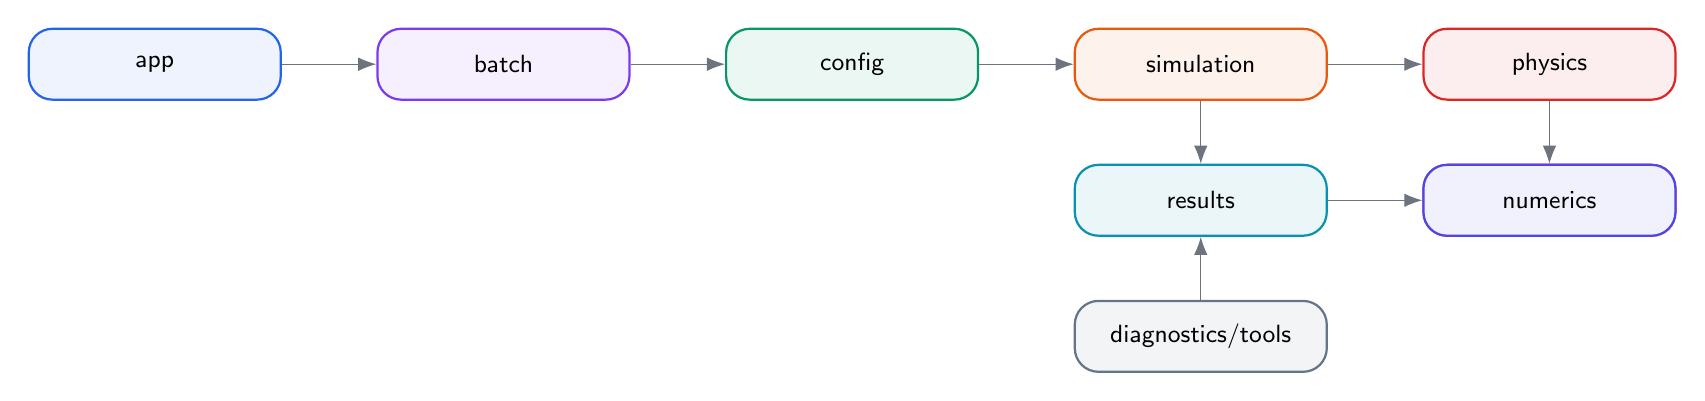
\begin{tikzpicture}[node distance=8mm and 12mm,every node/.style={font=\sffamily\small}]
\tikzstyle{chip}=[rounded corners=3mm,draw,line width=0.8pt,fill=white,minimum width=32mm,minimum height=9mm,align=center]
\node[chip,draw=appc,fill=appc!8] (app) {app};
\node[chip,draw=batchc,fill=batchc!8,right=of app] (batch) {batch};
\node[chip,draw=configc,fill=configc!8,right=of batch] (config) {config};
\node[chip,draw=simulationc,fill=simulationc!8,right=of config] (sim) {simulation};
\node[chip,draw=physicsc,fill=physicsc!8,right=of sim] (phys) {physics};
\node[chip,draw=resultsc,fill=resultsc!8,below=of sim] (res) {results};
\node[chip,draw=ioc,fill=ioc!8,right=of res] (io) {io};
\node[chip,draw=numericsc,fill=numericsc!8,below=of phys] (num) {numerics};
\node[chip,draw=diagnosticsc,fill=diagnosticsc!8,below=of res] (diag) {diagnostics/tools};
\draw[-{Latex[length=2.3mm]},ink!65] (app)--(batch);
\draw[-{Latex[length=2.3mm]},ink!65] (batch)--(config);
\draw[-{Latex[length=2.3mm]},ink!65] (config)--(sim);
\draw[-{Latex[length=2.3mm]},ink!65] (sim)--(phys);
\draw[-{Latex[length=2.3mm]},ink!65] (phys)--(num);
\draw[-{Latex[length=2.3mm]},ink!65] (sim)--(res);
\draw[-{Latex[length=2.3mm]},ink!65] (res)--(io);
\draw[-{Latex[length=2.3mm]},ink!65] (diag)--(res);
\end{tikzpicture}
\end{center}
\vspace{4mm}
\begin{tabularx}{\textwidth}{p{0.16\textwidth}Y p{0.20\textwidth}}
\toprule
\textbf{枝} & \textbf{大まかな責務} & \textbf{主な連携先}\\
\midrule
\Path{app} & run.py から呼ばれ、通常実行か一括実行かを判定し、適切なアプリケーション処理へ処理を流す。 & config, batch, simulation, results, io \\
\rowcolor{rowstripe}
\Path{batch} & CSV各行を設計ケースとして解釈し、設定反映、並列実行、進捗表示、batch\_summary 作成までを統括する。 & config, app.model\_sweep, io.excel \\
\Path{config} & JSON設定を読み、単位と値を検証し、物理コンポーネントとEngineを構築する。 & app, batch, physics.components \\
\rowcolor{rowstripe}
\Path{simulation} & タンク、インジェクタ、燃焼室、ノズルを一時刻ごとに評価し、状態ベクトルを時間発展させる。 & physics.components, results \\
\Path{physics} & materials, flow, components に分け、材料物性・流れ構成式・実体部品を混ぜない。 & simulation.rhs \\
\rowcolor{rowstripe}
\Path{results} & solutionとevent logから時系列表、summary、保存用データを作る。 & io \\
\Path{io} & Excel, JSON, text, filesystem操作を物理モデルから切り離す。 & app, batch, results \\
\rowcolor{rowstripe}
\Path{numerics} & 補間、root solve、最適化を物理モデルから切り離して提供する。 & physics.materials, flow \\
\Path{diagnostics} & 本計算ではなく、入力データ・表補間・比較グラフの検査を行う。 & tools \\
\rowcolor{rowstripe}
\Path{tools} & 本体ロジックをdiagnosticsへ委譲し、ユーザーが単独実行しやすい入口だけを持つ。 & diagnostics \\

\bottomrule
\end{tabularx}
\BranchTitle{appc}{app}{階層 {\bfseries\textcolor{levelone}{1}}: 実行入口を束ねる枝}{}
run.py から呼ばれ、通常実行か一括実行かを判定し、適切なアプリケーション処理へ処理を流す。

\begin{tabularx}{\textwidth}{p{0.14\textwidth}Y p{0.14\textwidth}Y}
\toprule
\textbf{読むもの} & プロジェクトルート、0\_Settings、0\_Batch\_Execution の有無 & \textbf{渡すもの} & model sweep の結果、または batch 実行結果 \\
\midrule
\textbf{連携先} & config, batch, simulation, results, io & \textbf{代表フロー} & run.py -> app.cli -> app.model\_sweep / batch.execution.executor \\
\bottomrule\end{tabularx}
\vspace{3mm}
\begin{minipage}[t]{0.36\textwidth}
\subsection*{この枝の内部木構造}
\begin{codepanel}\small
\begin{Verbatim}[fontsize=\small,commandchars=\\\{\}]
app/
  ├── sweep/
  ├── cli.py
  └── model_sweep.py
\end{Verbatim}
\end{codepanel}
\end{minipage}\hfill
\begin{minipage}[t]{0.60\textwidth}
\subsection*{下位枝・直接ファイルの役割}
\small\begin{tabularx}{\textwidth}{p{0.31\textwidth}Y}
\toprule\textbf{名前} & \textbf{この階層での識別}\\\midrule
\Path{app/sweep/} & 一つの設定セットに対し、指定されたインジェクタモデルを順にまたは並列に実行し、共通出力へ集約する。 \\
\rowcolor{rowstripe}
\Path{cli.py} & run.pyから呼ばれる最上位dispatcher。batch検出と通常sweepの分岐だけを担う。 \\
\Path{model_sweep.py} & 通常実行のモデルスイープ全体を統括する。SPI/HEM/Dyerの結果を共通出力へまとめる。 \\
\bottomrule\end{tabularx}
\end{minipage}
\vspace{3mm}\subsection*{直接ファイルの責務と主なAPI}
\small\begin{longtable}{p{0.22\textwidth}p{0.43\textwidth}p{0.18\textwidth}p{0.12\textwidth}}
\toprule\textbf{ファイル} & \textbf{責務} & \textbf{主なAPI} & \textbf{使われる時}\\
\midrule\endfirsthead\toprule\textbf{ファイル} & \textbf{責務} & \textbf{主なAPI} & \textbf{使われる時}\\\midrule\endhead
\Path{cli.py} & run.pyから呼ばれる最上位dispatcher。batch検出と通常sweepの分岐だけを担う。 & main() & run.py実行時 \\
\rowcolor{rowstripe}
\Path{model_sweep.py} & 通常実行のモデルスイープ全体を統括する。SPI/HEM/Dyerの結果を共通出力へまとめる。 & run\_injector\_model\_sweep() & 0\_Batch\_Executionがないとき \\
\bottomrule\end{longtable}
\BranchTitle{appc}{app/sweep}{階層 {\bfseries\textcolor{leveltwo}{2}}: SPI/HEM/Dyer の通常モデルスイープ}{}
一つの設定セットに対し、指定されたインジェクタモデルを順にまたは並列に実行し、共通出力へ集約する。

\begin{tabularx}{\textwidth}{p{0.14\textwidth}Y p{0.14\textwidth}Y}
\toprule
\textbf{読むもの} & 設定辞書、run\_models、thermo table 状態 & \textbf{渡すもの} & モデル別フォルダ、model\_summary、比較グラフ \\
\midrule
\textbf{連携先} & simulation.Engine, io, diagnostics & \textbf{代表フロー} & config -> worker -> Engine.solve -> results/io \\
\bottomrule\end{tabularx}
\vspace{3mm}
\begin{minipage}[t]{0.36\textwidth}
\subsection*{この枝の内部木構造}
\begin{codepanel}\small
\begin{Verbatim}[fontsize=\small,commandchars=\\\{\}]
app/sweep/
  ├── config.py
  ├── execution.py
  ├── io.py
  ├── status.py
  └── worker.py
\end{Verbatim}
\end{codepanel}
\end{minipage}\hfill
\begin{minipage}[t]{0.60\textwidth}
\subsection*{下位枝・直接ファイルの役割}
\small\begin{tabularx}{\textwidth}{p{0.31\textwidth}Y}
\toprule\textbf{名前} & \textbf{この階層での識別}\\\midrule
\Path{config.py} & sweep実行時のモデル選択、並列設定、thermo prewarm条件を解釈する。 \\
\rowcolor{rowstripe}
\Path{execution.py} & 逐次/並列にmodel workerを動かし、結果を回収する。 \\
\Path{io.py} & sweep出力フォルダ、settings copy、summary出力をまとめる。 \\
\rowcolor{rowstripe}
\Path{status.py} & モデルworkerのstatus JSONペイロードとprogress callbackを作る。 \\
\Path{worker.py} & 1つのインジェクタモデルを実行するworker単位。Engineのsolveと保存を呼ぶ。 \\
\bottomrule\end{tabularx}
\end{minipage}
\vspace{3mm}\subsection*{直接ファイルの責務と主なAPI}
\small\begin{longtable}{p{0.22\textwidth}p{0.43\textwidth}p{0.18\textwidth}p{0.12\textwidth}}
\toprule\textbf{ファイル} & \textbf{責務} & \textbf{主なAPI} & \textbf{使われる時}\\
\midrule\endfirsthead\toprule\textbf{ファイル} & \textbf{責務} & \textbf{主なAPI} & \textbf{使われる時}\\\midrule\endhead
\Path{config.py} & sweep実行時のモデル選択、並列設定、thermo prewarm条件を解釈する。 & \_set\_json\_value(), \_dedupe\_preserve\_order(), \_compact\_none(), \_prefixed\_filename(), \_planned\_injector\_models() ... & model\_sweep開始時 \\
\rowcolor{rowstripe}
\Path{execution.py} & 逐次/並列にmodel workerを動かし、結果を回収する。 & model\_parallel\_settings(), run\_models\_parallel(), run\_models\_sequential() & model\_sweep実行中 \\
\Path{io.py} & sweep出力フォルダ、settings copy、summary出力をまとめる。 & Tee, model\_sweep\_output\_root(), prepare\_model\_sweep\_dirs(), write\_sweep\_common\_outputs() & sweep結果保存 \\
\rowcolor{rowstripe}
\Path{status.py} & モデルworkerのstatus JSONペイロードとprogress callbackを作る。 & \_write\_status(), \_design\_status\_payload(), \_make\_design\_status\_callback() & 並列sweepの進捗表示 \\
\Path{worker.py} & 1つのインジェクタモデルを実行するworker単位。Engineのsolveと保存を呼ぶ。 & \_run\_single\_model\_worker(), \_normalize\_model\_record() & SPI/HEM/Dyer各モデル実行 \\
\bottomrule\end{longtable}
\BranchTitle{batchc}{batch}{階層 {\bfseries\textcolor{levelone}{1}}: 一括入力CSVから複数設計を実行する枝}{}
CSV各行を設計ケースとして解釈し、設定反映、並列実行、進捗表示、batch\_summary 作成までを統括する。

\begin{tabularx}{\textwidth}{p{0.14\textwidth}Y p{0.14\textwidth}Y}
\toprule
\textbf{読むもの} & 0\_Batch\_Execution, Batch\_Execution\_Config.json, CSV & \textbf{渡すもの} & design別結果、batch\_summary.xlsx, input\_mapping, batch\_errors \\
\midrule
\textbf{連携先} & config, app.model\_sweep, io.excel & \textbf{代表フロー} & config -> input -> execution -> output -> io.excel.batch\_summary \\
\bottomrule\end{tabularx}
\vspace{3mm}
\begin{minipage}[t]{0.36\textwidth}
\subsection*{この枝の内部木構造}
\begin{codepanel}\small
\begin{Verbatim}[fontsize=\small,commandchars=\\\{\}]
batch/
  ├── config/
  ├── console/
  ├── execution/
  ├── input/
  ├── output/
  ├── planning/
  ├── constants.py
  └── model.py
\end{Verbatim}
\end{codepanel}
\end{minipage}\hfill
\begin{minipage}[t]{0.60\textwidth}
\subsection*{下位枝・直接ファイルの役割}
\small\begin{tabularx}{\textwidth}{p{0.31\textwidth}Y}
\toprule\textbf{名前} & \textbf{この階層での識別}\\\midrule
\Path{batch/config/} & batch設定ファイルを読み、CSV名、出力先、入力仕様の前提を整える。 \\
\rowcolor{rowstripe}
\Path{batch/console/} & 計算本体から独立して、準備activityと計算progressを読みやすく表示する。 \\
\Path{batch/execution/} & 各設計をworkerへ渡し、並列または逐次に実行し、進捗・結果・エラーを回収する。 \\
\rowcolor{rowstripe}
\Path{batch/input/} & Input\_Specification と Input\_Design\_Name を解釈し、CSVの値をJSON設定ツリーへ反映する。 \\
\Path{batch/output/} & モデル別summaryや入力ステータスから、batch\_summary とエラーレポート用データを作る。 \\
\rowcolor{rowstripe}
\Path{batch/planning/} & batch中でthermo tableを事前生成できるか、各設計で作るべきかを判断する。 \\
\Path{constants.py} & batch内で共有する定数名、status名などを持つ。 \\
\rowcolor{rowstripe}
\Path{model.py} & DesignCaseやBatchResultなどbatch用データ構造を定義する。 \\
\bottomrule\end{tabularx}
\end{minipage}
\vspace{3mm}\subsection*{直接ファイルの責務と主なAPI}
\small\begin{longtable}{p{0.22\textwidth}p{0.43\textwidth}p{0.18\textwidth}p{0.12\textwidth}}
\toprule\textbf{ファイル} & \textbf{責務} & \textbf{主なAPI} & \textbf{使われる時}\\
\midrule\endfirsthead\toprule\textbf{ファイル} & \textbf{責務} & \textbf{主なAPI} & \textbf{使われる時}\\\midrule\endhead
\Path{constants.py} & batch内で共有する定数名、status名などを持つ。 & - & batch全域 \\
\rowcolor{rowstripe}
\Path{model.py} & DesignCaseやBatchResultなどbatch用データ構造を定義する。 & InputColumnSpec, MonitorSpec, RowExecutionResult, BatchExecutionError & batch全域 \\
\bottomrule\end{longtable}
\BranchTitle{batchc}{batch/config}{階層 {\bfseries\textcolor{leveltwo}{2}}: 一括実行設定の読み込み}{}
batch設定ファイルを読み、CSV名、出力先、入力仕様の前提を整える。

\begin{tabularx}{\textwidth}{p{0.14\textwidth}Y p{0.14\textwidth}Y}
\toprule
\textbf{読むもの} & Batch\_Execution\_Config.json, 0\_Batch\_Execution & \textbf{渡すもの} & batch実行用の設定辞書とパス情報 \\
\midrule
\textbf{連携先} & batch.input, batch.execution & \textbf{代表フロー} & config -> input -> execution -> output -> io.excel.batch\_summary \\
\bottomrule\end{tabularx}
\vspace{3mm}
\begin{minipage}[t]{0.36\textwidth}
\subsection*{この枝の内部木構造}
\begin{codepanel}\small
\begin{Verbatim}[fontsize=\small,commandchars=\\\{\}]
batch/config/
  └── loader.py
\end{Verbatim}
\end{codepanel}
\end{minipage}\hfill
\begin{minipage}[t]{0.60\textwidth}
\subsection*{下位枝・直接ファイルの役割}
\small\begin{tabularx}{\textwidth}{p{0.31\textwidth}Y}
\toprule\textbf{名前} & \textbf{この階層での識別}\\\midrule
\Path{loader.py} & Batch\_Execution\_Config.jsonを読み、CSVパスとCopy\_Batch\_Executionを扱う。 \\
\bottomrule\end{tabularx}
\end{minipage}
\vspace{3mm}\subsection*{直接ファイルの責務と主なAPI}
\small\begin{longtable}{p{0.22\textwidth}p{0.43\textwidth}p{0.18\textwidth}p{0.12\textwidth}}
\toprule\textbf{ファイル} & \textbf{責務} & \textbf{主なAPI} & \textbf{使われる時}\\
\midrule\endfirsthead\toprule\textbf{ファイル} & \textbf{責務} & \textbf{主なAPI} & \textbf{使われる時}\\\midrule\endhead
\Path{loader.py} & Batch\_Execution\_Config.jsonを読み、CSVパスとCopy\_Batch\_Executionを扱う。 & \_read\_json(), \_batch\_csv\_basename(), detect\_batch\_execution(), \_copy\_batch\_execution\_dir() & batch準備 \\
\bottomrule\end{longtable}
\BranchTitle{batchc}{batch/input}{階層 {\bfseries\textcolor{leveltwo}{2}}: CSV行を設計ケースへ変換する枝}{}
Input\_Specification と Input\_Design\_Name を解釈し、CSVの値をJSON設定ツリーへ反映する。

\begin{tabularx}{\textwidth}{p{0.14\textwidth}Y p{0.14\textwidth}Y}
\toprule
\textbf{読むもの} & CSV DataFrame, Input\_Specification, design name列 & \textbf{渡すもの} & 設計ID、設計名、反映済み設定、入力セルステータス \\
\midrule
\textbf{連携先} & config.units, config.validation & \textbf{代表フロー} & CSV row -> unit conversion -> settings override -> validation cell status \\
\bottomrule\end{tabularx}
\vspace{3mm}
\begin{minipage}[t]{0.36\textwidth}
\subsection*{この枝の内部木構造}
\begin{codepanel}\small
\begin{Verbatim}[fontsize=\small,commandchars=\\\{\}]
batch/input/
  ├── design_name.py
  ├── destinations.py
  ├── row_config.py
  └── specs.py
\end{Verbatim}
\end{codepanel}
\end{minipage}\hfill
\begin{minipage}[t]{0.60\textwidth}
\subsection*{下位枝・直接ファイルの役割}
\small\begin{tabularx}{\textwidth}{p{0.31\textwidth}Y}
\toprule\textbf{名前} & \textbf{この階層での識別}\\\midrule
\Path{design_name.py} & Input\_Design\_Name列から設計名を読み、ファイル名安全な表記へsanitizeする。 \\
\rowcolor{rowstripe}
\Path{destinations.py} & Input\_Specificationの宛先JSONパスを解決する。 \\
\Path{row_config.py} & CSV 1行を設定辞書へ反映し、InputErrorをセル位置へ戻す。 \\
\rowcolor{rowstripe}
\Path{specs.py} & Input\_Specification, Input\_Design\_Name, Monitored\_Valuesを読み取る。 \\
\bottomrule\end{tabularx}
\end{minipage}
\vspace{3mm}\subsection*{直接ファイルの責務と主なAPI}
\small\begin{longtable}{p{0.22\textwidth}p{0.43\textwidth}p{0.18\textwidth}p{0.12\textwidth}}
\toprule\textbf{ファイル} & \textbf{責務} & \textbf{主なAPI} & \textbf{使われる時}\\
\midrule\endfirsthead\toprule\textbf{ファイル} & \textbf{責務} & \textbf{主なAPI} & \textbf{使われる時}\\\midrule\endhead
\Path{design_name.py} & Input\_Design\_Name列から設計名を読み、ファイル名安全な表記へsanitizeする。 & \_sanitize\_design\_name(), \_design\_label(), \_display\_design\_label() & CSV読み込み後 \\
\rowcolor{rowstripe}
\Path{destinations.py} & Input\_Specificationの宛先JSONパスを解決する。 & \_get\_destination\_node(), \_get\_destination\_unit(), \_set\_destination\_value(), \_normalized\_destination(), \_columns\_for\_destinations() & CSV値反映時 \\
\Path{row_config.py} & CSV 1行を設定辞書へ反映し、InputErrorをセル位置へ戻す。 & \_prepare\_row\_config(), \_infer\_input\_validation\_rejections() & 各Design準備 \\
\rowcolor{rowstripe}
\Path{specs.py} & Input\_Specification, Input\_Design\_Name, Monitored\_Valuesを読み取る。 & \_collect\_input\_specs(), \_collect\_design\_name\_column(), \_design\_names\_from\_csv(), \_design\_labels\_from\_names(), \_collect\_monitor\_specs() & batch準備 \\
\bottomrule\end{longtable}
\BranchTitle{batchc}{batch/planning}{階層 {\bfseries\textcolor{leveltwo}{2}}: 実行前の計画とthermo準備判断}{}
batch中でthermo tableを事前生成できるか、各設計で作るべきかを判断する。

\begin{tabularx}{\textwidth}{p{0.14\textwidth}Y p{0.14\textwidth}Y}
\toprule
\textbf{読むもの} & 入力仕様とCEA signatureに関わる設定 & \textbf{渡すもの} & prewarm可否、実行計画 \\
\midrule
\textbf{連携先} & batch.execution, chamber thermochemistry & \textbf{代表フロー} & config -> input -> execution -> output -> io.excel.batch\_summary \\
\bottomrule\end{tabularx}
\vspace{3mm}
\begin{minipage}[t]{0.36\textwidth}
\subsection*{この枝の内部木構造}
\begin{codepanel}\small
\begin{Verbatim}[fontsize=\small,commandchars=\\\{\}]
batch/planning/
  └── thermo.py
\end{Verbatim}
\end{codepanel}
\end{minipage}\hfill
\begin{minipage}[t]{0.60\textwidth}
\subsection*{下位枝・直接ファイルの役割}
\small\begin{tabularx}{\textwidth}{p{0.31\textwidth}Y}
\toprule\textbf{名前} & \textbf{この階層での識別}\\\midrule
\Path{thermo.py} & batch入力がthermo signatureを変え得るかを見てprewarm可否を判断する。 \\
\bottomrule\end{tabularx}
\end{minipage}
\vspace{3mm}\subsection*{直接ファイルの責務と主なAPI}
\small\begin{longtable}{p{0.22\textwidth}p{0.43\textwidth}p{0.18\textwidth}p{0.12\textwidth}}
\toprule\textbf{ファイル} & \textbf{責務} & \textbf{主なAPI} & \textbf{使われる時}\\
\midrule\endfirsthead\toprule\textbf{ファイル} & \textbf{責務} & \textbf{主なAPI} & \textbf{使われる時}\\\midrule\endhead
\Path{thermo.py} & batch入力がthermo signatureを変え得るかを見てprewarm可否を判断する。 & \_batch\_overrides\_thermo\_table\_signature() & batch準備 \\
\bottomrule\end{longtable}
\BranchTitle{batchc}{batch/execution}{階層 {\bfseries\textcolor{leveltwo}{2}}: 設計ケースの実行管理}{}
各設計をworkerへ渡し、並列または逐次に実行し、進捗・結果・エラーを回収する。

\begin{tabularx}{\textwidth}{p{0.14\textwidth}Y p{0.14\textwidth}Y}
\toprule
\textbf{読むもの} & 設計ケース、ベース設定、実行モード & \textbf{渡すもの} & 設計別summary、worker status、error rows \\
\midrule
\textbf{連携先} & app.model\_sweep, batch.console, batch.output & \textbf{代表フロー} & preparation -> worker\_count -> parallel/sequential -> progress\_monitor -> artifacts \\
\bottomrule\end{tabularx}
\vspace{3mm}
\begin{minipage}[t]{0.36\textwidth}
\subsection*{この枝の内部木構造}
\begin{codepanel}\small
\begin{Verbatim}[fontsize=\small,commandchars=\\\{\}]
batch/execution/
  ├── executor.py
  ├── layout.py
  ├── parallel.py
  ├── preparation.py
  ├── progress_monitor.py
  ├── results.py
  ├── sequential.py
  ├── worker.py
  └── worker_count.py
\end{Verbatim}
\end{codepanel}
\end{minipage}\hfill
\begin{minipage}[t]{0.60\textwidth}
\subsection*{下位枝・直接ファイルの役割}
\small\begin{tabularx}{\textwidth}{p{0.31\textwidth}Y}
\toprule\textbf{名前} & \textbf{この階層での識別}\\\midrule
\Path{executor.py} & batch全体の高レベル入口。準備、実行、出力の各枝を順に呼ぶ。 \\
\rowcolor{rowstripe}
\Path{layout.py} & 設計ID/モデル別の出力フォルダ構造を決める。 \\
\Path{parallel.py} & 複数設計をProcessPool等で並列実行する。 \\
\rowcolor{rowstripe}
\Path{preparation.py} & batch出力root、入力CSV、設計名、入力仕様など実行前準備をまとめる。 \\
\Path{progress_monitor.py} & parallel/sequential実行中にworker statusを読んでconsoleへ渡す。 \\
\rowcolor{rowstripe}
\Path{results.py} & workerから戻る成功/失敗結果の形を整える。 \\
\Path{sequential.py} & 設計を一つずつ順番に実行する。デバッグ時に有用。 \\
\rowcolor{rowstripe}
\Path{worker.py} & 1設計ケースを実行するworker本体。入力エラー時の扱いもここで分岐する。 \\
\Path{worker_count.py} & 利用するworker数を設計数・設定値から決める。 \\
\bottomrule\end{tabularx}
\end{minipage}
\vspace{3mm}\subsection*{直接ファイルの責務と主なAPI}
\small\begin{longtable}{p{0.22\textwidth}p{0.43\textwidth}p{0.18\textwidth}p{0.12\textwidth}}
\toprule\textbf{ファイル} & \textbf{責務} & \textbf{主なAPI} & \textbf{使われる時}\\
\midrule\endfirsthead\toprule\textbf{ファイル} & \textbf{責務} & \textbf{主なAPI} & \textbf{使われる時}\\\midrule\endhead
\Path{executor.py} & batch全体の高レベル入口。準備、実行、出力の各枝を順に呼ぶ。 & run\_batch\_execution() & run\_batch\_execution \\
\rowcolor{rowstripe}
\Path{layout.py} & 設計ID/モデル別の出力フォルダ構造を決める。 & write\_settings\_dir\_from\_config(), set\_json\_value(), prepare\_worker\_config(), ensure\_design\_layout() & worker開始前 \\
\Path{parallel.py} & 複数設計をProcessPool等で並列実行する。 & \_parallel\_failure\_result(), \_run\_parallel\_designs() & design\_parallel有効時 \\
\rowcolor{rowstripe}
\Path{preparation.py} & batch出力root、入力CSV、設計名、入力仕様など実行前準備をまとめる。 & prepare\_batch\_result\_root(), print\_batch\_header(), prewarm\_or\_explain\_thermo\_cache() & batch開始直後 \\
\Path{progress_monitor.py} & parallel/sequential実行中にworker statusを読んでconsoleへ渡す。 & progress\_line\_for\_pending() & batch実行中 \\
\rowcolor{rowstripe}
\Path{results.py} & workerから戻る成功/失敗結果の形を整える。 & input\_error\_result(), sweep\_result\_to\_row(), run\_error\_result() & worker完了時 \\
\Path{sequential.py} & 設計を一つずつ順番に実行する。デバッグ時に有用。 & \_run\_sequential\_designs() & design\_parallel無効時 \\
\rowcolor{rowstripe}
\Path{worker.py} & 1設計ケースを実行するworker本体。入力エラー時の扱いもここで分岐する。 & \_execute\_design(), \_execute\_design\_worker() & 各Design worker \\
\Path{worker_count.py} & 利用するworker数を設計数・設定値から決める。 & \_select\_design\_worker\_count() & parallel実行前 \\
\bottomrule\end{longtable}
\BranchTitle{batchc}{batch/console}{階層 {\bfseries\textcolor{leveltwo}{2}}: 一括実行中の表示を担う枝}{}
計算本体から独立して、準備activityと計算progressを読みやすく表示する。

\begin{tabularx}{\textwidth}{p{0.14\textwidth}Y p{0.14\textwidth}Y}
\toprule
\textbf{読むもの} & worker status JSON、進捗単位 & \textbf{渡すもの} & コンソール表示文字列 \\
\midrule
\textbf{連携先} & batch.execution.progress\_monitor & \textbf{代表フロー} & worker status JSON -> activity/progress\_units -> bars -> console line \\
\bottomrule\end{tabularx}
\vspace{3mm}
\begin{minipage}[t]{0.36\textwidth}
\subsection*{この枝の内部木構造}
\begin{codepanel}\small
\begin{Verbatim}[fontsize=\small,commandchars=\\\{\}]
batch/console/
  ├── activity.py
  ├── bars.py
  ├── progress_units.py
  └── status_io.py
\end{Verbatim}
\end{codepanel}
\end{minipage}\hfill
\begin{minipage}[t]{0.60\textwidth}
\subsection*{下位枝・直接ファイルの役割}
\small\begin{tabularx}{\textwidth}{p{0.31\textwidth}Y}
\toprule\textbf{名前} & \textbf{この階層での識別}\\\midrule
\Path{activity.py} & 準備フェーズだけに表示するactivityのマイルストーンを決める。25/25到達保証もここに関わる。 \\
\rowcolor{rowstripe}
\Path{bars.py} & activity用のドットバー、progress用のシャープバーなど文字バーの整形だけを担う。 \\
\Path{progress_units.py} & 設計内のSPI/HEM/Dyer進捗をbatch全体の進捗単位へ換算する。 \\
\rowcolor{rowstripe}
\Path{status_io.py} & worker status JSONを読み書きする。表示側とworker側の共有ファイル境界。 \\
\bottomrule\end{tabularx}
\end{minipage}
\vspace{3mm}\subsection*{直接ファイルの責務と主なAPI}
\small\begin{longtable}{p{0.22\textwidth}p{0.43\textwidth}p{0.18\textwidth}p{0.12\textwidth}}
\toprule\textbf{ファイル} & \textbf{責務} & \textbf{主なAPI} & \textbf{使われる時}\\
\midrule\endfirsthead\toprule\textbf{ファイル} & \textbf{責務} & \textbf{主なAPI} & \textbf{使われる時}\\\midrule\endhead
\Path{activity.py} & 準備フェーズだけに表示するactivityのマイルストーンを決める。25/25到達保証もここに関わる。 & preparation\_activity\_count(), activity\_milestone\_counts(), activity\_milestone\_lines() & progressが動き始める前 \\
\rowcolor{rowstripe}
\Path{bars.py} & activity用のドットバー、progress用のシャープバーなど文字バーの整形だけを担う。 & format\_progress\_bar(), format\_activity\_bar() & console表示生成 \\
\Path{progress_units.py} & 設計内のSPI/HEM/Dyer進捗をbatch全体の進捗単位へ換算する。 & design\_progress\_units() & progress percent計算 \\
\rowcolor{rowstripe}
\Path{status_io.py} & worker status JSONを読み書きする。表示側とworker側の共有ファイル境界。 & write\_status\_file(), read\_status\_snapshot() & worker status更新/監視 \\
\bottomrule\end{longtable}

\begin{note}
この枝は、親の batch から見ると「表示」に見えるが、内部では読み書き、進捗単位化、activity判定、バー整形が分離されている。したがって、console表示を変えるときは、何を変えるのかを先に決める。状態ファイル形式なら status_io、進捗率なら progress_units、表示タイミングなら activity、見た目なら bars を見る。
\end{note}
\BranchTitle{batchc}{batch/output}{階層 {\bfseries\textcolor{leveltwo}{2}}: batch成果物の組み立て}{}
モデル別summaryや入力ステータスから、batch\_summary とエラーレポート用データを作る。

\begin{tabularx}{\textwidth}{p{0.14\textwidth}Y p{0.14\textwidth}Y}
\toprule
\textbf{読むもの} & 各worker結果、入力マッピング、エラー情報 & \textbf{渡すもの} & batch\_summary用行、batch\_errors、input\_mapping \\
\midrule
\textbf{連携先} & io.excel.batch\_summary, io.text & \textbf{代表フロー} & worker results -> model rows/error reports -> batch\_summary writer \\
\bottomrule\end{tabularx}
\vspace{3mm}
\begin{minipage}[t]{0.36\textwidth}
\subsection*{この枝の内部木構造}
\begin{codepanel}\small
\begin{Verbatim}[fontsize=\small,commandchars=\\\{\}]
batch/output/
  ├── artifacts.py
  ├── model_rows.py
  └── reports.py
\end{Verbatim}
\end{codepanel}
\end{minipage}\hfill
\begin{minipage}[t]{0.60\textwidth}
\subsection*{下位枝・直接ファイルの役割}
\small\begin{tabularx}{\textwidth}{p{0.31\textwidth}Y}
\toprule\textbf{名前} & \textbf{この階層での識別}\\\midrule
\Path{artifacts.py} & batch全体の成果物保存をまとめて呼ぶ。 \\
\rowcolor{rowstripe}
\Path{model_rows.py} & 各モデルsummaryからbatch\_summaryシート行を作る。 \\
\Path{reports.py} & batch\_errors.json/txtやinput\_mappingの保存を担当する。 \\
\bottomrule\end{tabularx}
\end{minipage}
\vspace{3mm}\subsection*{直接ファイルの責務と主なAPI}
\small\begin{longtable}{p{0.22\textwidth}p{0.43\textwidth}p{0.18\textwidth}p{0.12\textwidth}}
\toprule\textbf{ファイル} & \textbf{責務} & \textbf{主なAPI} & \textbf{使われる時}\\
\midrule\endfirsthead\toprule\textbf{ファイル} & \textbf{責務} & \textbf{主なAPI} & \textbf{使われる時}\\\midrule\endhead
\Path{artifacts.py} & batch全体の成果物保存をまとめて呼ぶ。 & write\_batch\_outputs(), cleanup\_worker\_status\_files() & batch終了時 \\
\rowcolor{rowstripe}
\Path{model_rows.py} & 各モデルsummaryからbatch\_summaryシート行を作る。 & build\_model\_sheet\_rows() & batch summary作成前 \\
\Path{reports.py} & batch\_errors.json/txtやinput\_mappingの保存を担当する。 & \_write\_input\_mapping\_text(), \_write\_design\_error\_files(), \_write\_batch\_errors() & batch終了時 \\
\bottomrule\end{longtable}

% -----------------------------------------------------------------------------
% User-facing batch configuration and CSV specification.
% -----------------------------------------------------------------------------
\BranchTitle{batchc}{0\_Batch\_Execution}{入力CSVから複数設計を作るユーザー設定枝}{}
ここは \Path{src/hybrid_motor_sim/batch/} の実装ではなく、ユーザーが直接編集する \Path{0_Batch_Execution/} の仕様である。通常実行では読まれず、\Path{0_Batch_Execution/Batch_Execution_Config.json} と指定CSVが存在すると一括実行モードに入る。

\begin{tabularx}{\textwidth}{p{0.15\textwidth}Y p{0.15\textwidth}Y}
\toprule
\textbf{読むもの} & \Path{Batch_Execution_Config.json}, 指定CSV & \textbf{渡すもの} & designごとの上書き済みsettings、design name、monitor指定 \\
\midrule
\textbf{主な連携} & \Path{batch/config}, \Path{batch/input}, \Path{batch/execution}, \Path{io/excel/batch_summary} & \textbf{代表フロー} & JSON仕様読取 -> CSV列検証 -> 単位変換 -> 設定反映 -> 各design実行 -> workbook監視値抽出 \\
\bottomrule\end{tabularx}

\begin{visual}
\centering
\begin{tikzpicture}[node distance=8mm and 12mm,every node/.style={font=\sffamily\small}]
\tikzstyle{box}=[rounded corners=2mm,draw,line width=0.7pt,fill=white,minimum width=34mm,minimum height=9mm,align=center]
\node[box,draw=batchc,fill=batchc!8] (cfg) {Batch\_Execution\_Config.json};
\node[box,draw=batchc,fill=batchc!8,right=of cfg] (csv) {CSV各行};
\node[box,draw=configc,fill=configc!8,right=of csv] (settings) {0\_Settingsへ反映};
\node[box,draw=simulationc,fill=simulationc!8,right=of settings] (run) {各design実行};
\node[box,draw=ioc,fill=ioc!8,below=of run] (book) {timeseries workbook};
\node[box,draw=ioc,fill=ioc!8,left=of book] (summary) {batch\_summary.xlsx};
\draw[-{Latex[length=2.3mm]},ink!65] (cfg)--(csv);
\draw[-{Latex[length=2.3mm]},ink!65] (csv)--(settings);
\draw[-{Latex[length=2.3mm]},ink!65] (settings)--(run);
\draw[-{Latex[length=2.3mm]},ink!65] (run)--(book);
\draw[-{Latex[length=2.3mm]},ink!65] (book)--(summary);
\end{tikzpicture}
\end{visual}

\subsection*{内部木構造とファイル}
\begin{codepanel}\small
\begin{Verbatim}[fontsize=\small]
0_Batch_Execution/
  ├── Batch_Execution_Config.json
  └── <File_Name>.csv
\end{Verbatim}
\end{codepanel}

\begin{longtable}{p{0.24\textwidth}p{0.33\textwidth}p{0.35\textwidth}}
\toprule\textbf{要素} & \textbf{役割} & \textbf{プログラムへの影響}\\
\midrule\endfirsthead\toprule\textbf{要素} & \textbf{役割} & \textbf{プログラムへの影響}\\\midrule\endhead
\Path{File_Name.Value} & 入力CSV名。拡張子は指定せず、\Code{.csv} として解決する。 & \Path{batch/config/loader.py} がCSVパスを決める。 \\
\rowcolor{rowstripe}
\Path{Input_Specification.Value} & CSV列名ごとに、入力単位と反映先Destinationを定義する。 & \Path{batch/input/specs.py} が列を検証し、\Path{batch/input/row_config.py} が行ごとのsettingsを作る。 \\
\Path{Input_Design_Name.Value} & 任意のCSV列をdesign名として使う。nullなら数値IDのみ。 & designフォルダ名・console表示・batch summaryのName列に反映される。 \\
\rowcolor{rowstripe}
\Path{Monitored_Values.Value} & batch\_summaryへ抜き出すworkbookシート、列、単位、集計位置を定義する。 & \Path{io/excel/batch_summary/monitoring.py} がtimeseries workbookから値を抽出する。 \\
\bottomrule\end{longtable}

\BranchTitle{batchc}{Batch\_Execution\_Config.json/Input\_Specification}{CSV列を0\_Settingsへ接続する仕様}{}
\Path{Input_Specification.Value} は「CSV列名 -> 反映先設定値」の対応表である。CSV列名は完全一致で照合される。列名の末尾に \Code{[mm]} や \Code{[MPa]} が含まれていても、それは人間に読みやすい名前であり、実際の変換にはJSON側の \Path{Unit} が使われる。

\begin{tabularx}{\textwidth}{p{0.17\textwidth}Y p{0.17\textwidth}Y}
\toprule
\textbf{読むもの} & CSV列名、CSVセル値、\Path{Unit}, \Path{Destination} & \textbf{渡すもの} & 変換済みのsettings dict \\
\midrule
\textbf{主な連携} & \Path{config/units}, \Path{batch/input/destinations.py} & \textbf{代表フロー} & CSV値 -> 単位変換 -> DestinationのValueを書き換え \\
\bottomrule\end{tabularx}

\begin{visual}
\centering
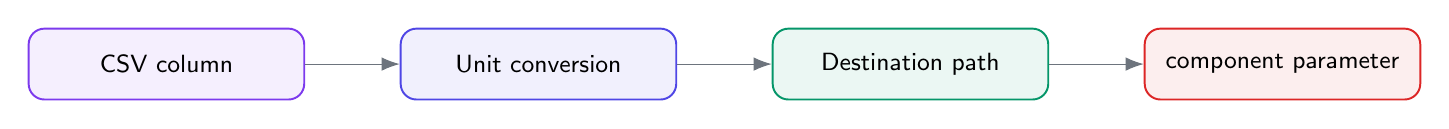
\begin{tikzpicture}[node distance=8mm and 12mm,every node/.style={font=\sffamily\small}]
\tikzstyle{box}=[rounded corners=2mm,draw,line width=0.7pt,fill=white,minimum width=35mm,minimum height=9mm,align=center]
\node[box,draw=batchc,fill=batchc!8] (col) {CSV column};
\node[box,draw=numericsc,fill=numericsc!8,right=of col] (unit) {Unit conversion};
\node[box,draw=configc,fill=configc!8,right=of unit] (dest) {Destination path};
\node[box,draw=physicsc,fill=physicsc!8,right=of dest] (model) {component parameter};
\draw[-{Latex[length=2.3mm]},ink!65] (col)--(unit);
\draw[-{Latex[length=2.3mm]},ink!65] (unit)--(dest);
\draw[-{Latex[length=2.3mm]},ink!65] (dest)--(model);
\end{tikzpicture}
\end{visual}

\begin{codepanel}\small
\begin{Verbatim}[fontsize=\small]
"ノズルスロート径 d_t [mm]": {
    "Unit": "[mm]",
    "Destination": "7_Nozzle/d_t"
}
\end{Verbatim}
\end{codepanel}

この指定は、\Path{File_Name} で指定した入力CSVから \Code{ノズルスロート径 d_t [mm]} に完全一致する列を探し、その列の各セル値を \Code{[mm]} として解釈し、\Path{0_Settings/7_Nozzle.json} の \Path{d_t/Value} を書き換える、という意味である。書き換え時には、CSV側の \Path{Unit} から、Destination先に書かれている \Path{Unit} へ自動変換される。

\begin{longtable}{p{0.22\textwidth}p{0.30\textwidth}p{0.40\textwidth}}
\toprule\textbf{キー} & \textbf{意味} & \textbf{実装上の扱い}\\
\midrule\endfirsthead\toprule\textbf{キー} & \textbf{意味} & \textbf{実装上の扱い}\\\midrule\endhead
CSV列名 & \Code{"ノズルスロート径 d_t [mm]"} のような辞書キー。 & 入力CSVの列名と完全一致で照合する。列がなければInputError。\\
\rowcolor{rowstripe}
\Path{Unit} & CSVセル値をどの単位として読むか。 & \Path{config/units} がDestination側Unitへ変換する。\\
\Path{Destination} & 書き換える設定値の場所。 & \Code{7_Nozzle/d_t} は \Path{0_Settings/7_Nozzle.json} の \Path{d_t/Value} を意味する。\\
\bottomrule\end{longtable}

\begin{note}
\textbf{Destinationの規則。} \Path{7_Nozzle/d_t} のように、ファイル番号名から始まり、JSON内の枝を \Code{/} で降りる。Destinationの最後が \Path{Value/Unit/Definition/Note} 形式の設定項目なら、その \Path{Value} だけを書き換える。存在しない枝、\Path{Unit} を持たない枝、空欄セルはInputErrorとして扱われる。
\end{note}

\BranchTitle{batchc}{Batch\_Execution\_Config.json/Input\_Design\_Name と CSV仕様}{設計IDに人間が読める名前を添える}{}
CSVの各行は自動的に \Code{Design ID = 1, 2, ...} として扱われる。\Path{Input_Design_Name.Value} にCSV列名を指定すると、その列の値がdesign名として読み込まれ、結果フォルダやconsole表示では \Code{<ID>_<Name>} 形式になる。一方、\Path{batch_summary.xlsx} ではID列は数値だけを保持し、Name列に設計名を分離して表示する。

\begin{longtable}{p{0.25\textwidth}p{0.35\textwidth}p{0.32\textwidth}}
\toprule\textbf{項目} & \textbf{仕様} & \textbf{注意}\\
\midrule\endfirsthead\toprule\textbf{項目} & \textbf{仕様} & \textbf{注意}\\\midrule\endhead
CSV encoding & pandasで読み込めるCSV。現在の同梱例はBOM付きUTF-8でも読める。 & 列名は完全一致。全角・半角・空白の違いに注意する。 \\
\rowcolor{rowstripe}
行の意味 & 1行が1設計。全行に対してSPI/HEM/Dyer等の指定モデルを実行する。 & 途中の行だけ失敗してもbatch全体は可能な限り継続する。 \\
Design ID & CSVの行順に1から自動採番する。 & batch summaryの第一列は常に数値ID。 \\
\rowcolor{rowstripe}
Design Name & 任意列。危険文字、空白、長すぎる文字列はファイル名安全化される。 & \Code{<>:"/\textbackslash{}|?*} と制御文字は \Code{_} に置換される。 \\
入力セルの色 & 受理済みは薄青、Design Nameは薄紫、InputErrorは薄赤。 & cross-field validationで落ちた値も対応セルが薄赤になる。 \\
\bottomrule\end{longtable}

\begin{codepanel}\small
\begin{Verbatim}[fontsize=\small]
"Input_Design_Name": {
    "Value": "Design_Name"
}
\end{Verbatim}
\end{codepanel}

\Path{Value} が \Code{null} なら、設計名機能は無効になり、結果フォルダやconsole表示は数値IDだけを使う。列名が指定されている場合は、入力CSVからその列を完全一致で探し、各行の値をファイル名として安全な文字列へ整形したうえで \Code{<ID>_<Name>} の表示に使う。

\BranchTitle{batchc}{Batch\_Execution\_Config.json/Monitored\_Values}{batch\_summaryへ抜き出す値の仕様}{}
\Path{Monitored_Values.Value} は、各設計・各モデルの時系列Excelから、比較したい値を \Path{batch_summary.xlsx} へ集約する仕様である。\Path{Source} は \Code{Sheet/Header} 形式で、時系列workbook内のシート名とヘッダー名を完全一致で参照する。\Path{Location} は「どのフェーズの、どの統計量か」を表す。

\begin{tabularx}{\textwidth}{p{0.15\textwidth}Y p{0.15\textwidth}Y}
\toprule
\textbf{読むもの} & timeseries workbookのシート名・列名、Unit、Location & \textbf{渡すもの} & batch summaryのモデル別シート列 \\
\midrule
\textbf{主な連携} & \Path{results/timeseries/workbook_schema.py}, \Path{io/excel/batch_summary/monitoring.py} & \textbf{代表フロー} & Sheet/Header -> phase filter -> statistic -> unit conversion -> cell value \\
\bottomrule\end{tabularx}

\begin{codepanel}\small
\begin{Verbatim}[fontsize=\small]
"特性排気速度[m/s]": {
    "Unit": "[m/s]",
    "Source": "Results/c_star[m/s]",
    "Location": "average@liquid"
}

"燃料ピッチ慣性[kg*m^2]": {
    "Unit": "[kg*m^2]",
    "Source": "For_Mechanics/I_pitch_fuel[kg*m^2]",
    "Location": "last@all"
}
\end{Verbatim}
\end{codepanel}

この指定は、\Path{batch_summary.xlsx} に指定ラベルの列を追加し、各設計・各モデルの時系列Excelから \Code{Results/c_star[m/s]} や \Path{For_Mechanics/I_pitch_fuel[kg*m^2]} を読み、指定 \Path{Unit} へ単位変換したうえで、\Code{average@liquid} などの操作により値を算出する、という意味である。\Path{Source} の \Code{/} は最初の1個だけをシート名と列名の区切りとして扱うため、\Path{kg/m^2/s} のように列名側に \Code{/} を含む単位も使用できる。

\begin{longtable}{p{0.22\textwidth}p{0.28\textwidth}p{0.40\textwidth}}
\toprule\textbf{構成要素} & \textbf{選択肢} & \textbf{意味}\\
\midrule\endfirsthead\toprule\textbf{構成要素} & \textbf{選択肢} & \textbf{意味}\\\midrule\endhead
\Path{Source} & \Code{Results/<header>}, \Code{For_Mechanics/<header>} & timeseries workbookのシート名とヘッダー名を完全一致で指定する。シート名を省略した指定は無効である。\\
\rowcolor{rowstripe}
統計操作 & \Code{first}, \Code{last}, \Code{average}, \Code{max}, \Code{min} & \Code{first/last} は対象範囲の端点を取る。\Code{average/max/min} は数値化できない値、NaN、非有限値を除外してから計算する。\\
フェーズ範囲 & \Code{all}, \Code{liquid}, \Code{gas} & \Code{all} は全時系列、\Code{liquid} は \Path{tank_phase} が液相共存、\Code{gas} は気相ブローダウンの行だけを使う。\\
\rowcolor{rowstripe}
\Path{Location} & \Code{<operation>@<phase>} & 使用可能な指定は \Code{(first,last,average,max,min)} と \Code{(all,liquid,gas)} の直積すべてである。\\
\bottomrule\end{longtable}

\begin{note}
\textbf{探索リストを別に持たない。} 監視値抽出は、実際に生成されたtimeseries workbookのシート名とヘッダー名に対して完全一致で行う。シート名は \Path{results/timeseries/workbook_schema.py} の \Path{RESULTS_SHEET_NAME} と \Path{MECHANICS_SHEET_NAME} が単一ソースであり、抽出側が独自の列名リストを持つことはない。Source不一致や抽出不能な指定は、計算そのものの失敗ではなく \Path{output_error} として扱われる。
\end{note}

\BranchTitle{configc}{config}{階層 {\bfseries\textcolor{levelone}{1}}: 設定ロード・検証・モデル構築の枝}{}
JSON設定を読み、単位と値を検証し、物理コンポーネントとEngineを構築する。

\begin{tabularx}{\textwidth}{p{0.14\textwidth}Y p{0.14\textwidth}Y}
\toprule
\textbf{読むもの} & 0\_Settings/*.json & \textbf{渡すもの} & Engine, run\_models, runtime configuration \\
\midrule
\textbf{連携先} & app, batch, physics.components & \textbf{代表フロー} & loading -> validation -> factory -> Engine \\
\bottomrule\end{tabularx}
\vspace{3mm}
\begin{minipage}[t]{0.36\textwidth}
\subsection*{この枝の内部木構造}
\begin{codepanel}\small
\begin{Verbatim}[fontsize=\small,commandchars=\\\{\}]
config/
  ├── factory/
  ├── loading/
  ├── units/
  └── validation/
\end{Verbatim}
\end{codepanel}
\end{minipage}\hfill
\begin{minipage}[t]{0.60\textwidth}
\subsection*{下位枝・直接ファイルの役割}
\small\begin{tabularx}{\textwidth}{p{0.31\textwidth}Y}
\toprule\textbf{名前} & \textbf{この階層での識別}\\\midrule
\Path{config/factory/} & Oxidizer/Tank/Injector/Chamber/Nozzle/Engineを生成する。物理式は持たず依存注入を行う。 \\
\rowcolor{rowstripe}
\Path{config/loading/} & プロジェクトルート、設定ディレクトリ、JSON設定群を確定する。 \\
\Path{config/units/} & mm, MPa, \%, L などの表記をSI内部値へ変換し、空欄・null・単位不一致も扱う。 \\
\rowcolor{rowstripe}
\Path{config/validation/} & 幾何寸法、充填率、効率、モデル選択など、ユーザー入力として危険な値を検出する。 \\
\bottomrule\end{tabularx}
\end{minipage}
\BranchTitle{configc}{config/loading}{階層 {\bfseries\textcolor{leveltwo}{2}}: 設定ファイルとパス解決}{}
プロジェクトルート、設定ディレクトリ、JSON設定群を確定する。

\begin{tabularx}{\textwidth}{p{0.14\textwidth}Y p{0.14\textwidth}Y}
\toprule
\textbf{読むもの} & project\_root, settings\_dir & \textbf{渡すもの} & settings dict, resolved paths \\
\midrule
\textbf{連携先} & config.factory & \textbf{代表フロー} & loading -> validation -> factory -> Engine \\
\bottomrule\end{tabularx}
\vspace{3mm}
\begin{minipage}[t]{0.36\textwidth}
\subsection*{この枝の内部木構造}
\begin{codepanel}\small
\begin{Verbatim}[fontsize=\small,commandchars=\\\{\}]
config/loading/
  ├── project.py
  └── settings.py
\end{Verbatim}
\end{codepanel}
\end{minipage}\hfill
\begin{minipage}[t]{0.60\textwidth}
\subsection*{下位枝・直接ファイルの役割}
\small\begin{tabularx}{\textwidth}{p{0.31\textwidth}Y}
\toprule\textbf{名前} & \textbf{この階層での識別}\\\midrule
\Path{project.py} & プロジェクトルートとsettings\_dirの解決を行う。 \\
\rowcolor{rowstripe}
\Path{settings.py} & 0\_Settings配下のJSONを読み込む。 \\
\bottomrule\end{tabularx}
\end{minipage}
\vspace{3mm}\subsection*{直接ファイルの責務と主なAPI}
\small\begin{longtable}{p{0.22\textwidth}p{0.43\textwidth}p{0.18\textwidth}p{0.12\textwidth}}
\toprule\textbf{ファイル} & \textbf{責務} & \textbf{主なAPI} & \textbf{使われる時}\\
\midrule\endfirsthead\toprule\textbf{ファイル} & \textbf{責務} & \textbf{主なAPI} & \textbf{使われる時}\\\midrule\endhead
\Path{project.py} & プロジェクトルートとsettings\_dirの解決を行う。 & find\_project\_root(), resolve\_settings\_dir() & 起動時 \\
\rowcolor{rowstripe}
\Path{settings.py} & 0\_Settings配下のJSONを読み込む。 & read\_json(), load\_settings() & config build前 \\
\bottomrule\end{longtable}
\BranchTitle{configc}{config/validation}{階層 {\bfseries\textcolor{leveltwo}{2}}: 設定値の妥当性検証}{}
幾何寸法、充填率、効率、モデル選択、設定JSONの書式など、ユーザー入力として危険な値を検出する。

\begin{tabularx}{\textwidth}{p{0.14\textwidth}Y p{0.14\textwidth}Y}
\toprule
\textbf{読むもの} & settings dict & \textbf{渡すもの} & Validation error または通過結果 \\
\midrule
\textbf{連携先} & batch.input, config.factory & \textbf{代表フロー} & loading -> validation -> factory -> Engine \\
\bottomrule\end{tabularx}
\vspace{3mm}
\begin{minipage}[t]{0.36\textwidth}
\subsection*{この枝の内部木構造}
\begin{codepanel}\small
\begin{Verbatim}[fontsize=\small,commandchars=\\\{\}]
config/validation/
  └── settings.py
\end{Verbatim}
\end{codepanel}
\end{minipage}\hfill
\begin{minipage}[t]{0.60\textwidth}
\subsection*{下位枝・直接ファイルの役割}
\small\begin{tabularx}{\textwidth}{p{0.31\textwidth}Y}
\toprule\textbf{名前} & \textbf{この階層での識別}\\\midrule
\Path{settings.py} & 幾何・充填率・効率・モデル名に加え、\Path{Value} と並列なJSONキーの許可範囲、\Path{Options} の有無、リスト選択式の値を検証する。 \\
\bottomrule\end{tabularx}
\end{minipage}
\vspace{3mm}\subsection*{直接ファイルの責務と主なAPI}
\small\begin{longtable}{p{0.22\textwidth}p{0.43\textwidth}p{0.18\textwidth}p{0.12\textwidth}}
\toprule\textbf{ファイル} & \textbf{責務} & \textbf{主なAPI} & \textbf{使われる時}\\
\midrule\endfirsthead\toprule\textbf{ファイル} & \textbf{責務} & \textbf{主なAPI} & \textbf{使われる時}\\\midrule\endhead
\Path{settings.py} & \Path{0_Information} を除くsettings項目で、\Path{Value}, \Path{Options}, \Path{Unit}, \Path{Definition}, \Path{Note*} 以外の並列キーを禁止し、選択式項目の \Path{Options} と入力値を検証する。 & validate\_config\_values() & component生成前 \\
\bottomrule\end{longtable}

\BranchTitle{configc}{config/units}{階層 {\bfseries\textcolor{leveltwo}{2}}: CSV入力とJSON設定をつなぐ単位変換}{}
mm, MPa, \%, L などの表記をSI内部値へ変換し、空欄・null・単位不一致も扱う。

\begin{tabularx}{\textwidth}{p{0.14\textwidth}Y p{0.14\textwidth}Y}
\toprule
\textbf{読むもの} & CSVセル値、Unit文字列 & \textbf{渡すもの} & SI値、変換済み設定値、セルエラー \\
\midrule
\textbf{連携先} & batch.input.row\_config & \textbf{代表フロー} & loading -> validation -> factory -> Engine \\
\bottomrule\end{tabularx}
\vspace{3mm}
\begin{minipage}[t]{0.36\textwidth}
\subsection*{この枝の内部木構造}
\begin{codepanel}\small
\begin{Verbatim}[fontsize=\small,commandchars=\\\{\}]
config/units/
  ├── blank.py
  ├── conversion.py
  ├── converters.py
  ├── errors.py
  ├── labels.py
  ├── parser.py
  ├── registry.py
  └── value.py
\end{Verbatim}
\end{codepanel}
\end{minipage}\hfill
\begin{minipage}[t]{0.60\textwidth}
\subsection*{下位枝・直接ファイルの役割}
\small\begin{tabularx}{\textwidth}{p{0.31\textwidth}Y}
\toprule\textbf{名前} & \textbf{この階層での識別}\\\midrule
\Path{blank.py} & 空欄、null、未指定の扱いを一箇所に集約する。 \\
\rowcolor{rowstripe}
\Path{conversion.py} & 実際の単位変換計算を行う。 \\
\Path{converters.py} & unit conversionのpublic facade。batch側のimport面を短く保つ。 \\
\rowcolor{rowstripe}
\Path{errors.py} & 単位変換エラー型とメッセージを扱う。 \\
\Path{labels.py} & 単位ラベルの正規化と表示名を扱う。 \\
\rowcolor{rowstripe}
\Path{parser.py} & Unit文字列やセル表現を解析する。 \\
\Path{registry.py} & 対応する単位ラベルとSI係数を登録する。 \\
\rowcolor{rowstripe}
\Path{value.py} & 値と単位の組を扱う小さな構造を提供する。 \\
\bottomrule\end{tabularx}
\end{minipage}
\vspace{3mm}\subsection*{直接ファイルの責務と主なAPI}
\small\begin{longtable}{p{0.22\textwidth}p{0.43\textwidth}p{0.18\textwidth}p{0.12\textwidth}}
\toprule\textbf{ファイル} & \textbf{責務} & \textbf{主なAPI} & \textbf{使われる時}\\
\midrule\endfirsthead\toprule\textbf{ファイル} & \textbf{責務} & \textbf{主なAPI} & \textbf{使われる時}\\\midrule\endhead
\Path{blank.py} & 空欄、null、未指定の扱いを一箇所に集約する。 & is\_blank() & CSVセル処理 \\
\rowcolor{rowstripe}
\Path{conversion.py} & 実際の単位変換計算を行う。 & conversion\_spec(), convert\_value() & CSV値反映時 \\
\Path{converters.py} & unit conversionのpublic facade。batch側のimport面を短く保つ。 & - & CSV値変換 \\
\rowcolor{rowstripe}
\Path{errors.py} & 単位変換エラー型とメッセージを扱う。 & UnitConversionError & 変換失敗時 \\
\Path{labels.py} & 単位ラベルの正規化と表示名を扱う。 & extract\_unit\_from\_label() & 変換前処理 \\
\rowcolor{rowstripe}
\Path{parser.py} & Unit文字列やセル表現を解析する。 & \_Parser, \_dims\_to\_tuple(), \_combine(), \_power(), normalize\_unit() ... & CSV読み込み時 \\
\Path{registry.py} & 対応する単位ラベルとSI係数を登録する。 & - & 変換時 \\
\rowcolor{rowstripe}
\Path{value.py} & 値と単位の組を扱う小さな構造を提供する。 & ParsedUnit, ConversionSpec, parse\_feet\_inches\_value() & 変換時 \\
\bottomrule\end{longtable}

\BranchTitle{configc}{config/units 仕様}{自動単位変換の文法・対応範囲・限界}{}
自動単位変換は、一括実行CSVの入力値と \Path{0_Settings} の \Path{Unit} を接続するための補助機能である。単発実行の \Path{0_Settings/*.json} を丸ごとSIへ変換する機能ではない。

\begin{tabularx}{\textwidth}{p{0.15\textwidth}Y p{0.15\textwidth}Y}
\toprule
\textbf{読むもの} & CSV側Unit、Destination側Unit、CSVセル値 & \textbf{渡すもの} & DestinationのValueへ入れる変換済み値 \\
\midrule
\textbf{主な連携} & \Path{batch/input/specs.py}, \Path{batch/input/row_config.py} & \textbf{代表フロー} & parse unit -> dimension check -> factor/offset -> Valueへ代入 \\
\bottomrule\end{tabularx}

\subsection*{単位式の文法}
\begin{longtable}{p{0.23\textwidth}p{0.30\textwidth}p{0.38\textwidth}}
\toprule\textbf{表記} & \textbf{例} & \textbf{説明}\\
\midrule\endfirsthead\toprule\textbf{表記} & \textbf{例} & \textbf{説明}\\\midrule\endhead
角括弧付き単位 & \Path{[mm]}, \Path{[MPa]}, \Path{[kg/(m^2*s)]} & CSV/JSONのUnit欄で使う基本形。 \\
\rowcolor{rowstripe}
乗算・除算 & \Path{[kg/(m^2*s)]}, \Path{[N*s]} & \Code{*}, \Code{/}, 括弧を使える。 \\
整数冪 & \Path{[m^2]}, \Path{[m^3]} & \Code{\textasciicircum{}2}, \Code{\textasciicircum{}3} のような整数冪に対応。 \\
\rowcolor{rowstripe}
無次元 & \Path{[-]} & 次元なし。次元付き単位とは変換不可。 \\
未定義 & \Path{...} & ファイル名やモデル名など、単位変換しない値。 \\
\rowcolor{rowstripe}
シンボリック & \Path{[(m/s)/(kg/(m^2*s))^n]} & \Code{\textasciicircum{}n} を含む単位は同一表記のみ許可。後退速度係数用。 \\
\bottomrule\end{longtable}


\subsection*{対応単位と接頭語}
\begin{longtable}{p{0.18\textwidth}p{0.28\textwidth}p{0.44\textwidth}}
\toprule\textbf{分類} & \textbf{対応単位} & \textbf{備考}\\
\midrule\endfirsthead\toprule\textbf{分類} & \textbf{対応単位} & \textbf{備考}\\\midrule\endhead
接頭語 & \Code{m, c, h, k, M} & それぞれ \Code{1e-3, 1e-2, 1e2, 1e3, 1e6} として解釈する。接頭語は、コード内でprefix可と登録された基底単位にだけ付けられる。\\
\rowcolor{rowstripe}
長さ & \Code{m, in, ft} とprefix付き長さ & \Code{mm, cm, km} などは \Code{m} に接頭語が付いたものとして扱う。\\
質量 & \Code{kg, g, t, lb} とprefix付き \Code{g, t} & \Code{kg} は基底単位として扱い、さらに \Code{kkg} のような接頭語は付けない。\\
\rowcolor{rowstripe}
時間 & \Code{s, min, h} & \Code{s} はSI単位だが接頭語を付けない。\Code{h} は時間単位として扱い、接頭語 \Code{h} (hecto) とはトークンとして区別して処理する。\\
力 & \Code{N, kgf, lbf} とprefix付き \Code{N} & \Code{N} は力カテゴリであり、\Path{kg*m/s^2} へ自動簡約しない。\\
\rowcolor{rowstripe}
圧力 & \Code{Pa, bar, atm, PSI, psi} とprefix付き \Code{Pa, bar} & \Code{MPa}, \Code{kPa}, \Code{mbar} などは接頭語として処理する。\\
体積 & \Path{m^3, L, cc} とprefix付き \Code{m, L} & \Path{cm^3} は \Path{(cm)^3} として解釈される。\Path{mL} も \Code{L} の接頭語付きとして扱う。\\
\rowcolor{rowstripe}
物質量 & \Code{mol} とprefix付き \Code{mol} & \Code{kmol}, \Code{mmol} などに対応する。\\
温度 & \Code{K, ℃} とprefix付き \Code{K} & \Code{℃ <-> K} の273.15 offset変換は単独温度のときだけ行う。\\
\rowcolor{rowstripe}
割合 & \Code{\%, vol\%, mol\%, wt\%} & \Code{\%} と各種割合単位の間は等倍変換可能。\Code{vol\% <-> mol\%} など異種割合同士はエラー。\\
\bottomrule\end{longtable}

\subsection*{単位式の文法と制限}
\begin{longtable}{p{0.24\textwidth}p{0.66\textwidth}}
\toprule\textbf{項目} & \textbf{仕様}\\
\midrule\endfirsthead\toprule\textbf{項目} & \textbf{仕様}\\\midrule\endhead
演算子 & 積 \Code{*}、除算 \Code{/}、整数べき \Code{\textasciicircum{}}、括弧に対応する。演算順序は通常の数式と同様に扱う。\\
\rowcolor{rowstripe}
接頭語の結合 & \Path{cm^2} は \Path{(cm)^2} と解釈する。接頭語は単位名と強く結びつく。\\
次元判定 & 長さ、質量、時間、力、圧力、体積、物質量、温度、割合などのカテゴリ指数が一致する場合だけ変換する。\\
\rowcolor{rowstripe}
SIへの完全簡約なし & \Code{N} と \Path{kg*m/s^2} は物理的には同じでも、この変換器では別カテゴリなので変換しない。登録された単位集合の範囲でだけ変換する。\\
温度offset & 単独の \Code{[℃]} と \Code{[K]} の相互変換だけ273.15を加減する。\Code{[℃/s]} のような組立単位では温度差として扱い、offset変換は行わない。\\
\rowcolor{rowstripe}
無次元と未定義 & \Code{[-]} は無次元量、\Code{...} は単位を定義しない値である。両者は区別され、互いに変換しない。\\
後退係数a & \Path{[(m/s)/(kg/(m^2*s))^n]} のように \Code{\textasciicircum{}n} を含むシンボリック単位は同一表記のみ等倍で通す。\Path{a} は \Path{n} に依存するため、一般単位変換対象外である。\\
\rowcolor{rowstripe}
feet-inch & \Code{\{ft\}'\{in\}} は特殊表記として認識されるが、batch変換での一般出力単位としては使わない。\\
\bottomrule\end{longtable}

\begin{note}
\textbf{安全側の考え方。} この単位変換器は、接頭語付きSI/一部SI併用単位と、実務で使う非SI単位を限定的に変換するための層である。物理式を使った換算、たとえば体積率から質量率への換算や、力を \Path{kg*m/s^2} に分解しての換算は行わない。変換不能な単位はInputErrorとして扱い、暗黙の誤変換を防ぐ。
\end{note}

\BranchTitle{configc}{config/factory}{階層 {\bfseries\textcolor{leveltwo}{2}}: 設定から実行可能オブジェクトを組み立てる枝}{}
Oxidizer、FeedSystem、Chamber、Nozzle、Engineを生成する。物理式は持たず、設定値の単位変換・正規化済み値をcomponentへ依存注入する。

\begin{tabularx}{\textwidth}{p{0.14\textwidth}Y p{0.14\textwidth}Y}
\toprule
\textbf{読むもの} & 検証済みsettings & \textbf{渡すもの} & Engineと各component \\
\midrule
\textbf{連携先} & physics.components, simulation.system & \textbf{代表フロー} & settings -> FeedSystem/Chamber/Nozzle -> Engine \\
\bottomrule\end{tabularx}

\begin{note}
\Path{config/factory/__init__.py} は、settings accessor と loading/validation 系の軽いAPIを即時に公開し、\Path{build_engine_from_config()} と \Path{build_engine_from_settings()} は呼び出し時に \Path{builder.py} を遅延importする。これにより、NIST CSV schema check のようにEngineを構築しない診断枝は、RocketCEAや物理component生成に依存せずに読み込める。
\end{note}
\vspace{3mm}
\begin{minipage}[t]{0.36\textwidth}
\subsection*{この枝の内部木構造}
\begin{codepanel}\small
\begin{Verbatim}[fontsize=\small,commandchars=\\\{\}]
config/factory/
  ├── accessors.py
  ├── builder.py
  ├── chamber.py
  ├── engine.py
  ├── feed_system.py
  ├── models.py
  └── nozzle.py
\end{Verbatim}
\end{codepanel}
\end{minipage}\hfill
\begin{minipage}[t]{0.60\textwidth}
\subsection*{下位枝・直接ファイルの役割}
\small\begin{tabularx}{\textwidth}{p{0.31\textwidth}Y}
\toprule\textbf{名前} & \textbf{この階層での識別}\\\midrule
\Path{accessors.py} & settings dictから必須値やsectionを安全に取り出す。 \\
\rowcolor{rowstripe}
\Path{builder.py} & settings読み込みからEngine構築までのpublic入口。 \\
\Path{chamber.py} & CEA, Fuel, ChamberOxidizer, Chamberを組み立てる。 \\
\rowcolor{rowstripe}
\Path{engine.py} & component bundleをEngineへ渡す最終構築。 \\
\Path{feed_system.py} & Oxidizer, Valve, Injectorを作り、\Path{FeedSystem} facadeへ結合する。 \\
\rowcolor{rowstripe}
\Path{models.py} & run\_modelsやinjector model名の正規化を行う。 \\
\Path{nozzle.py} & Nozzle幾何と環境圧を構築する。 \\
\bottomrule\end{tabularx}
\end{minipage}
\vspace{3mm}\subsection*{直接ファイルの責務と主なAPI}
\small\begin{longtable}{p{0.22\textwidth}p{0.43\textwidth}p{0.18\textwidth}p{0.12\textwidth}}
\toprule\textbf{ファイル} & \textbf{責務} & \textbf{主なAPI} & \textbf{使われる時}\\
\midrule\endfirsthead\toprule\textbf{ファイル} & \textbf{責務} & \textbf{主なAPI} & \textbf{使われる時}\\\midrule\endhead
\Path{accessors.py} & settings dictから必須値やsectionを安全に取り出す。 & unwrap\_value(), require\_section(), require\_value(), require\_cstar\_efficiency(), safe\_str() ... & factory各所 \\
\rowcolor{rowstripe}
\Path{builder.py} & settings読み込みからEngine構築までのpublic入口。 & build\_engine\_from\_config(), build\_engine\_from\_settings() & app/batchから呼ばれる \\
\Path{chamber.py} & CEA, Fuel, ChamberOxidizer, Chamberを組み立てる。 & build\_chamber() & Engine構築 \\
\rowcolor{rowstripe}
\Path{engine.py} & component bundleをEngineへ渡す最終構築。 & build\_engine\_shell() & build\_engine\_from\_config \\
\Path{feed_system.py} & Oxidizer, Valve, Injector, FeedSystemを組み立てる。 & build\_feed\_system() & Engine構築 \\
\rowcolor{rowstripe}
\Path{models.py} & run\_modelsやinjector model名の正規化を行う。 & configured\_run\_models() & factory開始時 \\
\Path{nozzle.py} & Nozzle幾何と環境圧を構築する。 & build\_nozzle() & Engine構築 \\
\bottomrule\end{longtable}

% -----------------------------------------------------------------------------
% User-facing regular settings specification.
% -----------------------------------------------------------------------------

\BranchTitle{configc}{0\_Settings}{単発実行と一括実行の基準になるJSON設定枝}{}
\Path{0_Settings/} は、単発実行でも一括実行でも最終的に使われる基準設定である。一括実行ではCSVの各行がこの設定を複製し、\Path{Input_Specification} のDestinationだけを書き換える。つまり、CSVに載っていない値は \Path{0_Settings/} の値がそのまま使われる。

\begin{tabularx}{\textwidth}{p{0.15\textwidth}Y p{0.15\textwidth}Y}
\toprule
\textbf{読むもの} & \Path{0_Settings/*.json} & \textbf{渡すもの} & Engine, components, solver, output settings \\
\midrule
\textbf{主な連携} & \Path{config/loading}, \Path{config/validation}, \Path{config/factory} & \textbf{代表フロー} & JSONロード -> 値検証 -> component生成 -> simulation実行 \\
\bottomrule\end{tabularx}

\begin{visual}
\begin{minipage}[t]{0.35\textwidth}
\subsection*{この枝の内部木構造}
\begin{codepanel}\small
\begin{Verbatim}[fontsize=\small]
0_Settings/
  ├── 0_Information.json
  ├── 1_Oxidizer.json
  ├── 2_Fuel.json
  ├── 3_Tank.json
  ├── 4_Valve.json
  ├── 5_Injector.json
  ├── 6_Chamber.json
  ├── 7_Nozzle.json
  ├── 8_Environment.json
  └── 9_Config.json
\end{Verbatim}
\end{codepanel}
\end{minipage}\hfill
\begin{minipage}[t]{0.61\textwidth}
\subsection*{下位ファイルの役割}
\begin{tabularx}{\textwidth}{p{0.26\textwidth}Y}
\toprule\textbf{ファイル} & \textbf{主な責務}\\
\midrule
\Path{0_Information.json} & 設定対象名やメモを置く情報ファイル。入力値スキーマ検証の対象外。\\
\rowcolor{rowstripe}
\Path{1_Oxidizer.json} & N2O物性、PR-EOS、NASA9、RocketCEA酸化剤名を定義する。\\
\Path{2_Fuel.json} & fuel card、燃料後退係数、グレイン幾何を定義する。\\
\rowcolor{rowstripe}
\Path{3_Tank.json} & タンク初期圧・体積・充填指定・任意のタンク内径を定義する。\\
\Path{4_Valve.json} & 任意の全開feed valveを、Kvと代表内径、coupling設定、診断モデルで定義する。\\
\rowcolor{rowstripe}
\Path{5_Injector.json} & インジェクタ幾何、SPI/HEM/Dyer、気相SPI/PR設定を定義する。\\
\Path{6_Chamber.json} & 初期O/F、燃焼室体積、c*効率、thermo tableを定義する。\\
\rowcolor{rowstripe}
\Path{7_Nozzle.json} & スロート径、膨張比、ノズル分岐計算の幾何を定義する。\\
\Path{8_Environment.json} & 大気圧、環境温度など外部条件を定義する。\\
\rowcolor{rowstripe}
\Path{9_Config.json} & solver、並列実行、出力名、thermo table運用を定義する。\\
\bottomrule
\end{tabularx}
\end{minipage}
\end{visual}

\subsection*{設定項目の共通形式}
\begin{longtable}{p{0.19\textwidth}p{0.34\textwidth}p{0.38\textwidth}}
\toprule\textbf{キー} & \textbf{意味} & \textbf{扱い}\\
\midrule\endfirsthead\toprule\textbf{キー} & \textbf{意味} & \textbf{扱い}\\\midrule\endhead
\Path{Value} & 実際にプログラムが読む値。 & factoryは基本的にこの値だけを取り出す。一括実行ではここが書き換わる。 \\
\rowcolor{rowstripe}
\Path{Options} & 選択式項目で使用可能な値と、その値の意味。 & 文字列選択、null/number選択、リスト選択式に置く。true/false項目には付けない。 \\
\Path{Unit} & 人間向け単位情報と一括実行時の変換先単位。 & 単発実行では自動変換されず、各factory/componentが期待単位で解釈する。一括実行ではCSV UnitからこのUnitへ変換する。 \\
\rowcolor{rowstripe}
\Path{Definition} & 設定の短い意味。 & プログラム実行には使わない。ドキュメント・レビュー用。 \\
\Path{Note}, \Path{Note2}, ... & 注意点、適用範囲、設計上の意味。 & プログラム実行には使わない。複数の注意は \Path{Note2}, \Path{Note3} のように分ける。 \\
\bottomrule\end{longtable}

\begin{note}
\textbf{書式制約。} \Path{0_Information.json} を除き、\Path{Value} と並列に置けるキーは \Path{Options}, \Path{Unit}, \Path{Definition}, \Path{Note}, \Path{Note2}, ... だけである。\Path{source} などの非公式メモ項目や、\Path{Value} の中に混ざったメモ的要素は使わない。選択式項目では \Path{Options} を \Path{Value} の直後に置く。
\end{note}

\BranchTitle{configc}{0\_Settings/1\_Oxidizer.json}{N2O物性・CEA酸化剤名・PR-EOSを定義する}{}
酸化剤設定は、タンク飽和物性、気相PRブローダウン、インジェクタ流量、燃焼室CEA入力にまたがる。最も下層の物性データであり、ここを変更すると複数の物理枝へ波及する。

\begin{longtable}{p{0.30\textwidth}p{0.12\textwidth}p{0.23\textwidth}p{0.27\textwidth}}
\toprule\textbf{設定パス} & \textbf{Unit} & \textbf{内容} & \textbf{主な影響先}\\
\midrule\endfirsthead\toprule\textbf{設定パス} & \textbf{Unit} & \textbf{内容} & \textbf{主な影響先}\\\midrule\endhead
\Path{identity/Name} & \Path{...} & RocketCEAへ渡す酸化剤名。 & \Path{chamber/thermochemistry/cea/backend.py} \\
\rowcolor{rowstripe}
\Path{identity/MolW} & \Path{[g/mol]} & N2Oモル質量。 & タンクモル数、質量流量、燃焼室O/F、積算質量。 \\
\Path{thermophysical_data/Path_csv} & \Path{...} & NIST飽和物性CSVのパス。 & \Path{materials/nitrous_oxide/saturation/table.py} \\
\rowcolor{rowstripe}
\Path{thermophysical_data/T_min} & \Path{[K]} & 低温側イベント/範囲ガードの基準。 & タンク温度下限、物性表アクセス。 \\
\Path{thermophysical_data/saturation_bounds_policy} & \Path{...} & 飽和物性範囲外を \Code{clip} または \Code{raise} で扱う。 & ODE内部試行点、デバッグ時の異常検出。 \\
\rowcolor{rowstripe}
\Path{peng_robinson/T_c, p_c, omega} & \Path{[K], [Pa], [-]} & PR-EOSのN2O臨界物性。 & 気相タンク圧、PR気相流量、departure物性。 \\
\Path{ideal_gas_heat_capacity/NASA9/temperature_policy} & \Path{...} & NASA9係数の温度範囲外評価を \Code{extrapolate} または \Code{clip} で扱う。 & PR気相エネルギー式、PR等エントロピー流量。 \\
\rowcolor{rowstripe}
\Path{ideal_gas_heat_capacity/NASA9/low_temperature_interval/*} & various & 200--1000 KのNASA9係数区間。 & 理想気体比熱、エンタルピー、エントロピー。 \\
\Path{ideal_gas_heat_capacity/NASA9/high_temperature_interval/*} & various & 1000--6000 KのNASA9係数区間。 & 理想気体比熱、エンタルピー、エントロピー。 \\
\bottomrule\end{longtable}

\begin{note}
\textbf{NASA9係数の構造。} 各温度区間は \Path{T_min}, \Path{T_max}, \Path{coefficients} を持つ。係数配列の出典や並び順は \Path{Note} と \Path{Note2} に書き、\Path{source} のような非公式キーは使わない。
\end{note}

\BranchTitle{configc}{0\_Settings/2\_Fuel.json}{燃料カード・後退速度・グレイン幾何を定義する}{}
燃料設定は、RocketCEAのfuel card、燃料後退式、燃料ポート体積、燃料残量の計算に使われる。燃料密度はfuel card内の \Path{density_g_cc} が燃料グレイン密度としても使われる。

\begin{longtable}{p{0.27\textwidth}p{0.12\textwidth}p{0.23\textwidth}p{0.30\textwidth}}
\toprule\textbf{設定パス} & \textbf{Unit} & \textbf{内容} & \textbf{主な影響先}\\
\midrule\endfirsthead\toprule\textbf{設定パス} & \textbf{Unit} & \textbf{内容} & \textbf{主な影響先}\\\midrule\endhead
\Path{cea/fuel_card} & \Path{...} & fuel名、元素組成、生成エンタルピー、基準温度、密度。 & RocketCEA燃焼物性、燃焼温度、c*, Isp。 \\
\rowcolor{rowstripe}
\Path{regression_model/a} & \Path{[(m/s)/(kg/(m^2*s))^n]} & 後退速度係数。 & \Path{fuel_grain/model.py} の \Code{ddt_r}、燃料流量。 \\
\Path{regression_model/n} & \Path{[-]} & 後退速度指数。 & Go依存性、O/Fシフト、燃焼時間。 \\
\rowcolor{rowstripe}
\Path{grain_geometry/L} & \Path{[mm]} & 燃料長さ。 & ポート体積、燃料流量、燃料質量。 \\
\Path{grain_geometry/D} & \Path{[mm]} & 燃料外径。 & 最大ポート半径、fuel\_port\_limit event、スライバ率。 \\
\rowcolor{rowstripe}
\Path{grain_geometry/d_init} & \Path{[mm]} & 初期ポート径。 & 初期Go、燃料後退、初期燃料質量。 \\
\bottomrule\end{longtable}

\begin{note}
\textbf{入力検証。} \Path{D > d_init} は必須であり、違反すると \Path{config/validation/settings.py} でInputErrorになる。一括実行では対応するCSVセルが薄赤になる。
\end{note}

\BranchTitle{configc}{0\_Settings/3--5: Tank / Valve / Injector.json}{供給系の初期状態・任意バルブ・流量モデルを決める}{}
タンク、Valve、インジェクタは燃焼室へ入る酸化剤流量を支配するため、推力履歴へ最も直接的に効く枝である。Valveは無効なら供給系から外れ、有効なら液相時だけ全開Kv圧損要素としてTankとInjectorの間に入る。

\begin{longtable}{p{0.31\textwidth}p{0.12\textwidth}p{0.22\textwidth}p{0.27\textwidth}}
\toprule\textbf{設定パス} & \textbf{Unit} & \textbf{内容} & \textbf{主な影響先}\\
\midrule\endfirsthead\toprule\textbf{設定パス} & \textbf{Unit} & \textbf{内容} & \textbf{主な影響先}\\\midrule\endhead
\Path{3_Tank/p_init} & \Path{[MPa]} & 初期タンク圧。指定時は飽和表から初期温度を逆算する。 & タンク初期温度、初期飽和圧、初期流量。 \\
\rowcolor{rowstripe}
\Path{3_Tank/V} & \Path{[cc]} & タンク内部体積。 & 初期モル数、液相枯渇時刻、気相ブローダウン、For\_Mechanicsのタンク長さ導出。 \\
\Path{3_Tank/Tank_geometry/d} & \Path{[mm]} & 任意のタンク内径。nullならタンクCG・慣性列を出さない。 & For\_MechanicsのCG\_tank, I\_axis\_tank, I\_pitch\_tank。 \\
\rowcolor{rowstripe}
\Path{3_Tank/gas_liquid_ratio_Determinant/filling_rate} & \Path{[vol\%]} & 液相体積充填率。 & 初期液相/気相モル数。 \\
\Path{3_Tank/gas_liquid_ratio_Determinant/m_tot} & \Path{[kg]} & 総酸化剤質量指定。 & filling\_rateの代替。ちょうど一方だけを指定する。 \\
\rowcolor{rowstripe}
\Path{4_Valve/enabled} & \Path{[-]} & 全開Valve圧損モデルを有効にする。 & trueなら液相時に \Path{Tank -> Valve -> Injector}、falseなら \Path{Tank -> Injector}。 \\
\Path{4_Valve/Kv} & \Path{[m^3/h]} & 全開Valveの水基準流量係数。 & 液相Valve圧損、\Path{p_valve_exit[MPa]}、供給流量。 \\
\rowcolor{rowstripe}
\Path{4_Valve/d_inner} & \Path{[mm]} & 全開Valve流路の代表内径。 & \Path{G_valve}, \Path{u_valve}, Void Fraction診断。 \\
\Path{4_Valve/coupling/mode} & \Path{...} & \Code{predictor} または \Code{root}。 & Valve/Injector連成の計算方法と計算時間。 \\
\rowcolor{rowstripe}
\Path{4_Valve/diagnostics/void_fraction_models} & \Path{...} & 出力するボイド率診断モデルのリスト。 & \Path{Void_Fraction_HEM}, \Path{Void_Fraction_Zivi}, \Path{Void_Fraction_RA}。 \\
\Path{5_Injector/Cd} & \Path{[-]} & 有効流量係数。 & SPI/HEM/Dyer/gas flowの全流量に掛かる。 \\
\rowcolor{rowstripe}
\Path{5_Injector/d_orifice, N_orifice} & \Path{[mm], [-]} & オリフィス径と孔数。 & 総オリフィス面積、酸化剤流量。 \\
\Path{5_Injector/HEM_config/*} & various & HEM探索点、cache刻み、臨界テーブル設定。 & 二相流量の精度と速度。 \\
\rowcolor{rowstripe}
\Path{5_Injector/Gas_config/gas_blowdown_model} & \Path{...} & 気相フェーズ流量を \Code{SPI} または \Code{PR} から選ぶ。 & \Code{SPI} はタンク気相密度のBernoulli型近似、\Code{PR} は実在気体等エントロピー流れ。 \\
\Path{5_Injector/run_models} & \Path{...} & 通常実行で走らせる液相モデル群。 & app model sweep、batch内の各design実行。 \\
\bottomrule\end{longtable}

\begin{note}
\textbf{充填指定とValve仕様。} \Path{filling_rate} と \Path{m_tot} は、どちらか一方だけを非nullにする。Valveは液相時に固定仕様の \Code{Kv_SPI} 圧損要素として扱われ、気相ブローダウン時はpass-throughで \Path{p_valve_exit=p_tank} とする。
\end{note}

\BranchTitle{configc}{0\_Settings/6\_Chamber.json}{燃焼室蓄積・CEA・thermo tableを決める}{}
燃焼室設定は、燃焼室体積、初期O/F、c*効率、RocketCEA direct/table切替、thermo table範囲と診断基準を持つ。

\begin{longtable}{p{0.27\textwidth}p{0.12\textwidth}p{0.23\textwidth}p{0.30\textwidth}}
\toprule\textbf{設定パス} & \textbf{Unit} & \textbf{内容} & \textbf{主な影響先}\\
\midrule\endfirsthead\toprule\textbf{設定パス} & \textbf{Unit} & \textbf{内容} & \textbf{主な影響先}\\\midrule\endhead
\Path{6_Chamber/V_pre, V_post} & \Path{[cc]} & プレ/ポストチャンバー体積。 & 燃焼室体積、圧力応答。 \\
\rowcolor{rowstripe}
\Path{6_Chamber/OF_init} & \Path{[-]} & 初期の微小storage正則化用O/F。 & 立ち上がり時の数値安定性。 \\
\Path{6_Chamber/Cstar_Efficiency} & \Path{[-]} & 実効c*効率。 & \Path{Nozzle.flow} の有効温度、c*, 推力履歴。 \\
\rowcolor{rowstripe}
\Path{6_Chamber/thermo/mode} & \Path{...} & \Code{table} または \Code{cached_direct} の熱物性取得。 & ODE RHS速度と補間誤差。 \\
\Path{6_Chamber/thermo/dp_fd, dOF_fd} & \Path{[MPa], [-]} & CEA偏微分の有限差分幅。 & 圧力ODEの安定性。 \\
\rowcolor{rowstripe}
\Path{6_Chamber/thermo_table/*} & various & table範囲、格子数、cache、診断、auto refine。 & \Path{thermochemistry/table} 全体。 \\
\Path{6_Chamber/eval_bounds/*} & various & ODE評価中のp/O-F安全範囲。 & table/direct queryのクリップとfallback。 \\
\bottomrule\end{longtable}

\BranchTitle{configc}{0\_Settings/7--9: Nozzle / Environment / Config.json}{ノズル・環境・実行制御を決める}{}
これらは物理部品の幾何と、計算をどの範囲・精度・出力先で実行するかを決める。

\begin{longtable}{p{0.28\textwidth}p{0.12\textwidth}p{0.23\textwidth}p{0.29\textwidth}}
\toprule\textbf{設定パス} & \textbf{Unit} & \textbf{内容} & \textbf{主な影響先}\\
\midrule\endfirsthead\toprule\textbf{設定パス} & \textbf{Unit} & \textbf{内容} & \textbf{主な影響先}\\\midrule\endhead
\Path{7_Nozzle/eps} & \Path{[-]} & 膨張比 Ae/At。 & 出口面積、分岐判定、圧力推力。 \\
\rowcolor{rowstripe}
\Path{7_Nozzle/d_t} & \Path{[mm]} & スロート径。 & スロート面積、チョーク流量、燃焼室圧。 \\
\Path{8_Environment/p_amb} & \Path{[Pa]} & 周囲圧。 & ノズル背圧、推力圧力項、分岐判定。 \\
\rowcolor{rowstripe}
\Path{8_Environment/T_amb} & \Path{[K]} & 周囲温度。 & p\_init未指定時のタンク初期温度など。 \\
\Path{9_Config/tags/run_name} & \Path{...} & 結果フォルダ名へ付けるrun名。 & timestamp付きresult directory名。 \\
\rowcolor{rowstripe}
\Path{9_Config/tags/result_file_tag} & \Path{...} & timeseries/summary/event logファイル名へ付ける任意suffix。 & 結果ファイル名。 \\
\Path{9_Config/solver/t_step} & \Path{[s]} & 出力時系列の基本時間刻み。event時刻はこの等間隔列に追加される。 & \Path{Results}, \Path{For_Mechanics} の基本サンプリングと相境界行。 \\
\rowcolor{rowstripe}
\Path{9_Config/solver/t_max} & \Path{[s]} & 積分の最大時刻。 & solve\_ivpの上限と強制終了条件。 \\
\Path{9_Config/solver/rtol} & \Path{[-]} & solve\_ivp相対許容誤差。 & ODE解精度と計算時間。 \\
\rowcolor{rowstripe}
\Path{9_Config/solver/atol} & \Path{[-]} & solve\_ivp絶対許容誤差。 & 小さい状態量の誤差制御。 \\
\Path{9_Config/solver/max_step} & \Path{[s]} & solve\_ivp内部最大刻み。nullなら明示制限なし。 & event検出と計算時間。 \\
\rowcolor{rowstripe}
\Path{9_Config/events/F_cutoff} & \Path{[N]} & 推力cutoffイベントしきい値。 & \Path{thrust_cutoff} 停止判定。 \\
\Path{9_Config/events/liquid_eps} & \Path{[mol]} & 液相枯渇判定の残液モルしきい値。 & 液相->気相segment切替。 \\
\rowcolor{rowstripe}
\Path{9_Config/events/tank_temperature_margin} & \Path{[K]} & NIST下限へ近づいた時のclamp開始margin。 & タンク温度下限イベント。 \\
\Path{9_Config/events/thrust_event_enable_time} & \Path{[s]} & 推力cutoffを有効にする最小時刻。 & t=0近傍の誤停止防止。 \\
\rowcolor{rowstripe}
\Path{9_Config/progress/*} & various & 単発実行の進捗表示。 & console progress。 \\
\Path{9_Config/results/*} & various & 結果root、設定コピー有無。 & \Path{1_Results} と保存処理。 \\
\rowcolor{rowstripe}
\Path{9_Config/batch_run/*} & various & batch/design並列数とpolling。 & 一括実行の速度とconsole更新。 \\
\bottomrule\end{longtable}

\BranchTitle{simulationc}{simulation}{階層 {\bfseries\textcolor{levelone}{1}}: ODEシステムとして部品を結合する枝}{}
タンク、インジェクタ、燃焼室、ノズルを一時刻ごとに評価し、状態ベクトルを時間発展させる。

\begin{tabularx}{\textwidth}{p{0.14\textwidth}Y p{0.14\textwidth}Y}
\toprule
\textbf{読むもの} & Engine state, component models, solver config & \textbf{渡すもの} & solution, event log, solver stats \\
\midrule
\textbf{連携先} & physics.components, results & \textbf{代表フロー} & Engine.solve -> RHS evaluation -> component calls -> solver segments -> results \\
\bottomrule\end{tabularx}
\vspace{3mm}
\begin{minipage}[t]{0.36\textwidth}
\subsection*{この枝の内部木構造}
\begin{codepanel}\small
\begin{Verbatim}[fontsize=\small,commandchars=\\\{\}]
simulation/
  ├── events/
  ├── progress/
  ├── rhs/
  ├── solver/
  ├── state/
  └── system/
\end{Verbatim}
\end{codepanel}
\end{minipage}\hfill
\begin{minipage}[t]{0.60\textwidth}
\subsection*{下位枝・直接ファイルの役割}
\small\begin{tabularx}{\textwidth}{p{0.31\textwidth}Y}
\toprule\textbf{名前} & \textbf{この階層での識別}\\\midrule
\Path{simulation/events/} & 液相枯渇、温度下限、推力カットオフなどのevent関数を提供する。 \\
\rowcolor{rowstripe}
\Path{simulation/progress/} & 一つのモデル実行中の進捗を軽量に表示する。batchのconsoleとは別の枝。 \\
\Path{simulation/rhs/} & 一時刻で必要なタンク圧、インジェクタ流量、CEA物性、ノズル流量を評価し、状態微分へ変換する。 \\
\rowcolor{rowstripe}
\Path{simulation/solver/} & solve\_ivpを呼び、event後の状態整理、次segmentへの切替、event時刻を含む最終solution時刻列の組み立てを行う。 \\
\Path{simulation/state/} & ODE配列の添字、初期状態、Jacobian sparsityを集中管理する。 \\
\rowcolor{rowstripe}
\Path{simulation/system/} & 外部APIとしてのEngineを保持し、solve, summary, save\_resultsを下位モジュールへ委譲する。 \\
\bottomrule\end{tabularx}
\end{minipage}
\BranchTitle{simulationc}{simulation/system}{階層 {\bfseries\textcolor{leveltwo}{2}}: Engine facade}{}
外部APIとしてのEngineを保持し、solve, summary, save\_resultsを下位モジュールへ委譲する。

\begin{tabularx}{\textwidth}{p{0.14\textwidth}Y p{0.14\textwidth}Y}
\toprule
\textbf{読むもの} & component bundle, runtime config & \textbf{渡すもの} & solution and saved outputs \\
\midrule
\textbf{連携先} & simulation.solver, results, io & \textbf{代表フロー} & Engine.solve -> RHS evaluation -> component calls -> solver segments -> results \\
\bottomrule\end{tabularx}
\vspace{3mm}
\begin{minipage}[t]{0.36\textwidth}
\subsection*{この枝の内部木構造}
\begin{codepanel}\small
\begin{Verbatim}[fontsize=\small,commandchars=\\\{\}]
simulation/system/
  └── engine.py
\end{Verbatim}
\end{codepanel}
\end{minipage}\hfill
\begin{minipage}[t]{0.60\textwidth}
\subsection*{下位枝・直接ファイルの役割}
\small\begin{tabularx}{\textwidth}{p{0.31\textwidth}Y}
\toprule\textbf{名前} & \textbf{この階層での識別}\\\midrule
\Path{engine.py} & 外部から見るEngine facade。solveや保存を下位モジュールへ委譲する。 \\
\bottomrule\end{tabularx}
\end{minipage}
\vspace{3mm}\subsection*{直接ファイルの責務と主なAPI}
\small\begin{longtable}{p{0.22\textwidth}p{0.43\textwidth}p{0.18\textwidth}p{0.12\textwidth}}
\toprule\textbf{ファイル} & \textbf{責務} & \textbf{主なAPI} & \textbf{使われる時}\\
\midrule\endfirsthead\toprule\textbf{ファイル} & \textbf{責務} & \textbf{主なAPI} & \textbf{使われる時}\\\midrule\endhead
\Path{engine.py} & 外部から見るEngine facade。solveや保存を下位モジュールへ委譲する。 & Engine & app/model\_sweepから \\
\bottomrule\end{longtable}
\BranchTitle{simulationc}{simulation/state}{階層 {\bfseries\textcolor{leveltwo}{2}}: 状態ベクトルの意味と初期化}{}
ODE配列の添字、初期状態、Jacobian sparsityを集中管理する。

\begin{tabularx}{\textwidth}{p{0.14\textwidth}Y p{0.14\textwidth}Y}
\toprule
\textbf{読むもの} & component initial states & \textbf{渡すもの} & y0, indices, sparsity pattern \\
\midrule
\textbf{連携先} & simulation.rhs, solver & \textbf{代表フロー} & Engine.solve -> RHS evaluation -> component calls -> solver segments -> results \\
\bottomrule\end{tabularx}
\vspace{3mm}
\begin{minipage}[t]{0.36\textwidth}
\subsection*{この枝の内部木構造}
\begin{codepanel}\small
\begin{Verbatim}[fontsize=\small,commandchars=\\\{\}]
simulation/state/
  ├── indices.py
  ├── initialization.py
  └── jacobian.py
\end{Verbatim}
\end{codepanel}
\end{minipage}\hfill
\begin{minipage}[t]{0.60\textwidth}
\subsection*{下位枝・直接ファイルの役割}
\small\begin{tabularx}{\textwidth}{p{0.31\textwidth}Y}
\toprule\textbf{名前} & \textbf{この階層での識別}\\\midrule
\Path{indices.py} & 状態ベクトル配列の添字を一元管理する。 \\
\rowcolor{rowstripe}
\Path{initialization.py} & 各componentからODE初期状態y0を作る。 \\
\Path{jacobian.py} & Radau用のJacobian sparsity構造を作る。 \\
\bottomrule\end{tabularx}
\end{minipage}
\vspace{3mm}\subsection*{直接ファイルの責務と主なAPI}
\small\begin{longtable}{p{0.22\textwidth}p{0.43\textwidth}p{0.18\textwidth}p{0.12\textwidth}}
\toprule\textbf{ファイル} & \textbf{責務} & \textbf{主なAPI} & \textbf{使われる時}\\
\midrule\endfirsthead\toprule\textbf{ファイル} & \textbf{責務} & \textbf{主なAPI} & \textbf{使われる時}\\\midrule\endhead
\Path{indices.py} & 状態ベクトル配列の添字を一元管理する。 & - & RHS/solver全域 \\
\rowcolor{rowstripe}
\Path{initialization.py} & 各componentからODE初期状態y0を作る。 & initial\_engine\_state() & solve開始時 \\
\Path{jacobian.py} & Radau用のJacobian sparsity構造を作る。 & build\_engine\_jac\_sparsity() & solve\_ivp呼び出し前 \\
\bottomrule\end{longtable}
\BranchTitle{simulationc}{simulation/rhs}{階層 {\bfseries\textcolor{leveltwo}{2}}: ODE右辺の一時刻評価}{}
一時刻で必要なタンク圧、インジェクタ流量、CEA物性、ノズル流量を評価し、状態微分へ変換する。

\begin{tabularx}{\textwidth}{p{0.14\textwidth}Y p{0.14\textwidth}Y}
\toprule
\textbf{読むもの} & t, y, component models & \textbf{渡すもの} & dy/dt and step diagnostics \\
\midrule
\textbf{連携先} & physics.components & \textbf{代表フロー} & state vector -> feed\_system/chamber/nozzle -> derivatives \\
\bottomrule\end{tabularx}
\vspace{3mm}
\begin{minipage}[t]{0.36\textwidth}
\subsection*{この枝の内部木構造}
\begin{codepanel}\small
\begin{Verbatim}[fontsize=\small,commandchars=\\\{\}]
simulation/rhs/
  ├── derivatives.py
  └── evaluation.py
\end{Verbatim}
\end{codepanel}
\end{minipage}\hfill
\begin{minipage}[t]{0.60\textwidth}
\subsection*{下位枝・直接ファイルの役割}
\small\begin{tabularx}{\textwidth}{p{0.31\textwidth}Y}
\toprule\textbf{名前} & \textbf{この階層での識別}\\\midrule
\Path{derivatives.py} & StepEvaluationを状態微分dy/dtへ変換する。 \\
\rowcolor{rowstripe}
\Path{evaluation.py} & 一時刻に必要な中間量を評価し、重複計算を防ぐ。 \\
\bottomrule\end{tabularx}
\end{minipage}
\vspace{3mm}\subsection*{直接ファイルの責務と主なAPI}
\small\begin{longtable}{p{0.22\textwidth}p{0.43\textwidth}p{0.18\textwidth}p{0.12\textwidth}}
\toprule\textbf{ファイル} & \textbf{責務} & \textbf{主なAPI} & \textbf{使われる時}\\
\midrule\endfirsthead\toprule\textbf{ファイル} & \textbf{責務} & \textbf{主なAPI} & \textbf{使われる時}\\\midrule\endhead
\Path{derivatives.py} & StepEvaluationを状態微分dy/dtへ変換する。 & engine\_derivative() & ODE RHS内 \\
\rowcolor{rowstripe}
\Path{evaluation.py} & 一時刻に必要な中間量を評価し、重複計算を防ぐ。 & chamber\_nozzle\_flow() & ODE RHS内 \\
\bottomrule\end{longtable}
\BranchTitle{simulationc}{simulation/events}{階層 {\bfseries\textcolor{leveltwo}{2}}: 相切替・停止条件}{}
液相枯渇、温度下限、推力カットオフなどのevent関数を提供する。

\begin{tabularx}{\textwidth}{p{0.14\textwidth}Y p{0.14\textwidth}Y}
\toprule
\textbf{読むもの} & t, y, engine context & \textbf{渡すもの} & zero-crossing functions \\
\midrule
\textbf{連携先} & simulation.solver & \textbf{代表フロー} & Engine.solve -> RHS evaluation -> component calls -> solver segments -> results \\
\bottomrule\end{tabularx}
\vspace{3mm}
\begin{minipage}[t]{0.36\textwidth}
\subsection*{この枝の内部木構造}
\begin{codepanel}\small
\begin{Verbatim}[fontsize=\small,commandchars=\\\{\}]
simulation/events/
  └── engine_events.py
\end{Verbatim}
\end{codepanel}
\end{minipage}\hfill
\begin{minipage}[t]{0.60\textwidth}
\subsection*{下位枝・直接ファイルの役割}
\small\begin{tabularx}{\textwidth}{p{0.31\textwidth}Y}
\toprule\textbf{名前} & \textbf{この階層での識別}\\\midrule
\Path{engine_events.py} & 液相枯渇、温度下限、推力カットオフ等のevent関数を提供する。 \\
\bottomrule\end{tabularx}
\end{minipage}
\vspace{3mm}\subsection*{直接ファイルの責務と主なAPI}
\small\begin{longtable}{p{0.22\textwidth}p{0.43\textwidth}p{0.18\textwidth}p{0.12\textwidth}}
\toprule\textbf{ファイル} & \textbf{責務} & \textbf{主なAPI} & \textbf{使われる時}\\
\midrule\endfirsthead\toprule\textbf{ファイル} & \textbf{責務} & \textbf{主なAPI} & \textbf{使われる時}\\\midrule\endhead
\Path{engine_events.py} & 液相枯渇、温度下限、推力カットオフ等のevent関数を提供する。 & current\_phase(), thrust\_margin(), liquid\_remaining(), tank\_temperature\_margin\_event(), fuel\_port\_margin\_event() ... & solve\_ivp events \\
\bottomrule\end{longtable}
\BranchTitle{simulationc}{simulation/solver}{階層 {\bfseries\textcolor{leveltwo}{2}}: solve\_ivp segment loop}{}
solve\_ivpを呼び、event後の状態整理、次segmentへの切替、event時刻を含む最終solution時刻列の組み立てを行う。

\begin{tabularx}{\textwidth}{p{0.14\textwidth}Y p{0.14\textwidth}Y}
\toprule
\textbf{読むもの} & RHS, events, initial state & \textbf{渡すもの} & merged solution, event log \\
\midrule
\textbf{連携先} & simulation.events, state & \textbf{代表フロー} & initial segment -> solve\_ivp -> event handling -> next segment \\
\bottomrule\end{tabularx}
\vspace{3mm}
\begin{minipage}[t]{0.36\textwidth}
\subsection*{この枝の内部木構造}
\begin{codepanel}\small
\begin{Verbatim}[fontsize=\small,commandchars=\\\{\}]
simulation/solver/
  ├── engine_runner.py
  ├── event_handling.py
  ├── segments.py
  └── state.py
\end{Verbatim}
\end{codepanel}
\end{minipage}\hfill
\begin{minipage}[t]{0.60\textwidth}
\subsection*{下位枝・直接ファイルの役割}
\small\begin{tabularx}{\textwidth}{p{0.31\textwidth}Y}
\toprule\textbf{名前} & \textbf{この階層での識別}\\\midrule
\Path{engine_runner.py} & solve\_ivp segment loop本体。event発生ごとに状態を整える。 \\
\rowcolor{rowstripe}
\Path{event_handling.py} & event後のphase切替、clamp、停止判定を整理する。 \\
\Path{segments.py} & segmentごとの解を結合し、event境界時刻では後続segmentの状態を優先して評価する補助。 \\
\rowcolor{rowstripe}
\Path{state.py} & solver状態、統計、診断カウンタ初期化、event時刻を含む最終solutionの組み立てを担当する。 \\
\bottomrule\end{tabularx}
\end{minipage}
\vspace{3mm}\subsection*{直接ファイルの責務と主なAPI}
\small\begin{longtable}{p{0.22\textwidth}p{0.43\textwidth}p{0.18\textwidth}p{0.12\textwidth}}
\toprule\textbf{ファイル} & \textbf{責務} & \textbf{主なAPI} & \textbf{使われる時}\\
\midrule\endfirsthead\toprule\textbf{ファイル} & \textbf{責務} & \textbf{主なAPI} & \textbf{使われる時}\\\midrule\endhead
\Path{engine_runner.py} & solve\_ivp segment loop本体。event発生ごとに状態を整える。 & solve\_engine() & Engine.solve \\
\rowcolor{rowstripe}
\Path{event_handling.py} & event後のphase切替、clamp、停止判定を整理する。 & handle\_segment\_event() & event発生時 \\
\Path{segments.py} & segmentごとの解を結合し、event境界時刻では後続segmentの状態を優先して評価する。 & triggered\_event\_name(), termination\_category(), evaluate\_segments() & phase切替時 \\
\rowcolor{rowstripe}
\Path{state.py} & solver状態、統計、診断カウンタ初期化、event時刻を含む最終solutionの組み立てを担当する。 & reset\_engine\_solve\_state(), prepare\_initial\_segment\_state(), accumulate\_solver\_stats(), finalize\_engine\_solution() & solver内部 \\
\bottomrule\end{longtable}
\BranchTitle{simulationc}{simulation/progress}{階層 {\bfseries\textcolor{leveltwo}{2}}: 単発実行の進捗表示}{}
一つのモデル実行中の進捗を軽量に表示する。batchのconsoleとは別の枝。

\begin{tabularx}{\textwidth}{p{0.14\textwidth}Y p{0.14\textwidth}Y}
\toprule
\textbf{読むもの} & time/state progress & \textbf{渡すもの} & console progress line \\
\midrule
\textbf{連携先} & simulation.solver & \textbf{代表フロー} & Engine.solve -> RHS evaluation -> component calls -> solver segments -> results \\
\bottomrule\end{tabularx}
\vspace{3mm}
\begin{minipage}[t]{0.36\textwidth}
\subsection*{この枝の内部木構造}
\begin{codepanel}\small
\begin{Verbatim}[fontsize=\small,commandchars=\\\{\}]
simulation/progress/
  └── engine_progress.py
\end{Verbatim}
\end{codepanel}
\end{minipage}\hfill
\begin{minipage}[t]{0.60\textwidth}
\subsection*{下位枝・直接ファイルの役割}
\small\begin{tabularx}{\textwidth}{p{0.31\textwidth}Y}
\toprule\textbf{名前} & \textbf{この階層での識別}\\\midrule
\Path{engine_progress.py} & 単発Engine実行のprogress callbackを整形する。 \\
\bottomrule\end{tabularx}
\end{minipage}
\vspace{3mm}\subsection*{直接ファイルの責務と主なAPI}
\small\begin{longtable}{p{0.22\textwidth}p{0.43\textwidth}p{0.18\textwidth}p{0.12\textwidth}}
\toprule\textbf{ファイル} & \textbf{責務} & \textbf{主なAPI} & \textbf{使われる時}\\
\midrule\endfirsthead\toprule\textbf{ファイル} & \textbf{責務} & \textbf{主なAPI} & \textbf{使われる時}\\\midrule\endhead
\Path{engine_progress.py} & 単発Engine実行のprogress callbackを整形する。 & progress\_reset(), emit\_status\_progress(), format\_progress(), progress\_update(), progress\_message() & model worker実行時 \\
\bottomrule\end{longtable}
\BranchTitle{physicsc}{physics}{階層 {\bfseries\textcolor{levelone}{1}}: 物理モデルを三層に分離した枝}{}
materials, flow, components に分け、材料物性・流れ構成式・実体部品を混ぜない。

\begin{tabularx}{\textwidth}{p{0.14\textwidth}Y p{0.14\textwidth}Y}
\toprule
\textbf{読むもの} & state and parameters from simulation & \textbf{渡すもの} & pressure, flow, thrust, derivatives \\
\midrule
\textbf{連携先} & simulation.rhs & \textbf{代表フロー} & components -> flow/materials -> numerics \\
\bottomrule\end{tabularx}
\vspace{3mm}
\begin{minipage}[t]{0.36\textwidth}
\subsection*{この枝の内部木構造}
\begin{codepanel}\small
\begin{Verbatim}[fontsize=\small,commandchars=\\\{\}]
physics/
  ├── components/
  ├── flow/
  └── materials/
\end{Verbatim}
\end{codepanel}
\end{minipage}\hfill
\begin{minipage}[t]{0.60\textwidth}
\subsection*{下位枝・直接ファイルの役割}
\small\begin{tabularx}{\textwidth}{p{0.31\textwidth}Y}
\toprule\textbf{名前} & \textbf{この階層での識別}\\\midrule
\Path{physics/components/} & feed\_system, chamber, nozzleを外向きAPIとして束ね、simulationから呼ばれる境界になる。 \\
\rowcolor{rowstripe}
\Path{physics/flow/} & オリフィス、二相HEM/Dyer、PR実在気体流、ノズル理想気体関係を置く。 \\
\Path{physics/materials/} & N2Oなど、部品をまたいで使う物性データと状態方程式を置く。 \\
\bottomrule\end{tabularx}
\end{minipage}
\BranchTitle{physicsc}{physics/materials}{階層 {\bfseries\textcolor{leveltwo}{2}}: 材料物性}{}
N2Oなど、部品をまたいで使う物性データと状態方程式を置く。

\begin{tabularx}{\textwidth}{p{0.14\textwidth}Y p{0.14\textwidth}Y}
\toprule
\textbf{読むもの} & temperature, pressure, molar volume, CSV data & \textbf{渡すもの} & thermodynamic properties \\
\midrule
\textbf{連携先} & physics.flow, components & \textbf{代表フロー} & components -> flow/materials -> numerics \\
\bottomrule\end{tabularx}
\vspace{3mm}
\begin{minipage}[t]{0.36\textwidth}
\subsection*{この枝の内部木構造}
\begin{codepanel}\small
\begin{Verbatim}[fontsize=\small,commandchars=\\\{\}]
physics/materials/
  └── nitrous_oxide/
\end{Verbatim}
\end{codepanel}
\end{minipage}\hfill
\begin{minipage}[t]{0.60\textwidth}
\subsection*{下位枝・直接ファイルの役割}
\small\begin{tabularx}{\textwidth}{p{0.31\textwidth}Y}
\toprule\textbf{名前} & \textbf{この階層での識別}\\\midrule
\Path{physics/materials/nitrous_oxide/} & 飽和表、PR-EOS、NASA9理想気体物性を束ねる。 \\
\bottomrule\end{tabularx}
\end{minipage}
\BranchTitle{physicsc}{physics/materials/nitrous\_oxide}{階層 {\bfseries\textcolor{levelthree}{3}}: N2O物性の入口}{}
飽和表、PR-EOS、NASA9理想気体物性を束ねる。

\begin{tabularx}{\textwidth}{p{0.14\textwidth}Y p{0.14\textwidth}Y}
\toprule
\textbf{読むもの} & NIST CSV, PR constants, NASA9 coefficients & \textbf{渡すもの} & N2O property functions \\
\midrule
\textbf{連携先} & feed\_system tank/injector & \textbf{代表フロー} & components -> flow/materials -> numerics \\
\bottomrule\end{tabularx}
\vspace{3mm}
\begin{minipage}[t]{0.36\textwidth}
\subsection*{この枝の内部木構造}
\begin{codepanel}\small
\begin{Verbatim}[fontsize=\small,commandchars=\\\{\}]
physics/materials/nitrous_oxide/
  ├── eos/
  ├── ideal_gas/
  └── saturation/
\end{Verbatim}
\end{codepanel}
\end{minipage}\hfill
\begin{minipage}[t]{0.60\textwidth}
\subsection*{下位枝・直接ファイルの役割}
\small\begin{tabularx}{\textwidth}{p{0.31\textwidth}Y}
\toprule\textbf{名前} & \textbf{この階層での識別}\\\midrule
\Path{physics/materials/nitrous_oxide/eos/} & 気相単独タンクとPR気相オリフィスで使う実在気体圧力・departure量を提供する。 \\
\rowcolor{rowstripe}
\Path{physics/materials/nitrous_oxide/ideal_gas/} & PRの理想気体基準としてcp, h, sを一貫して計算する。 \\
\Path{physics/materials/nitrous_oxide/saturation/} & 液相共存タンクとHEMで使う飽和圧、飽和体積、エネルギー、微分を提供する。 \\
\bottomrule\end{tabularx}
\end{minipage}
\BranchTitle{physicsc}{physics/materials/nitrous\_oxide/saturation}{階層 {\bfseries\textcolor{levelfour}{4}}: NIST飽和物性表}{}
液相共存タンクとHEMで使う飽和圧、飽和体積、エネルギー、微分を提供する。

\begin{tabularx}{\textwidth}{p{0.14\textwidth}Y p{0.14\textwidth}Y}
\toprule
\textbf{読むもの} & NIST\_Chemistry.csv, bounds policy & \textbf{渡すもの} & psat(T), h\_l(T), u\_v(T), derivatives \\
\midrule
\textbf{連携先} & tank.liquid\_phase, two\_phase.hem & \textbf{代表フロー} & components -> flow/materials -> numerics \\
\bottomrule\end{tabularx}
\vspace{3mm}
\begin{minipage}[t]{0.36\textwidth}
\subsection*{この枝の内部木構造}
\begin{codepanel}\small
\begin{Verbatim}[fontsize=\small,commandchars=\\\{\}]
physics/materials/nitrous_oxide/saturation/
  ├── access.py
  ├── bounds.py
  ├── paths.py
  ├── schema.py
  └── table.py
\end{Verbatim}
\end{codepanel}
\end{minipage}\hfill
\begin{minipage}[t]{0.60\textwidth}
\subsection*{下位枝・直接ファイルの役割}
\small\begin{tabularx}{\textwidth}{p{0.31\textwidth}Y}
\toprule\textbf{名前} & \textbf{この階層での識別}\\\midrule
\Path{access.py} & bounds policyを適用した物性値・微分アクセスを提供する。 \\
\rowcolor{rowstripe}
\Path{bounds.py} & clip/raiseなど範囲外ポリシーを処理する。 \\
\Path{paths.py} & NIST CSVパスの解決を行う。 \\
\rowcolor{rowstripe}
\Path{schema.py} & NIST CSVに必要な列があるかを検査する。 \\
\Path{table.py} & NIST CSVから飽和表を読み、PCHIP補間器を構築する。 \\
\bottomrule\end{tabularx}
\end{minipage}
\vspace{3mm}\subsection*{直接ファイルの責務と主なAPI}
\small\begin{longtable}{p{0.22\textwidth}p{0.43\textwidth}p{0.18\textwidth}p{0.12\textwidth}}
\toprule\textbf{ファイル} & \textbf{責務} & \textbf{主なAPI} & \textbf{使われる時}\\
\midrule\endfirsthead\toprule\textbf{ファイル} & \textbf{責務} & \textbf{主なAPI} & \textbf{使われる時}\\\midrule\endhead
\Path{access.py} & bounds policyを適用した物性値・微分アクセスを提供する。 & SaturationAccessMixin & 物性評価時 \\
\rowcolor{rowstripe}
\Path{bounds.py} & clip/raiseなど範囲外ポリシーを処理する。 & sanitize\_coordinate(), ensure\_finite() & 物性評価時 \\
\Path{paths.py} & NIST CSVパスの解決を行う。 & resolve\_project\_relative\_path() & 設定読み込み時 \\
\rowcolor{rowstripe}
\Path{schema.py} & NIST CSVに必要な列があるかを検査する。 & validate\_required\_columns(), property\_column\_map(), csv\_schema\_info() & 起動診断 \\
\Path{table.py} & NIST CSVから飽和表を読み、PCHIP補間器を構築する。 & N2OSaturationTable & Oxidizer生成時 \\
\bottomrule\end{longtable}
\BranchTitle{physicsc}{physics/materials/nitrous\_oxide/eos}{階層 {\bfseries\textcolor{levelfour}{4}}: Peng-Robinson EOS}{}
気相単独タンクとPR気相オリフィスで使う実在気体圧力・departure量を提供する。

\begin{tabularx}{\textwidth}{p{0.14\textwidth}Y p{0.14\textwidth}Y}
\toprule
\textbf{読むもの} & T, molar volume & \textbf{渡すもの} & p, u\_dep, h\_dep, s\_dep, Cv corrections \\
\midrule
\textbf{連携先} & gas\_phase, real\_gas.isentropic\_orifice & \textbf{代表フロー} & components -> flow/materials -> numerics \\
\bottomrule\end{tabularx}
\vspace{3mm}
\begin{minipage}[t]{0.36\textwidth}
\subsection*{この枝の内部木構造}
\begin{codepanel}\small
\begin{Verbatim}[fontsize=\small,commandchars=\\\{\}]
physics/materials/nitrous_oxide/eos/
  └── peng_robinson.py
\end{Verbatim}
\end{codepanel}
\end{minipage}\hfill
\begin{minipage}[t]{0.60\textwidth}
\subsection*{下位枝・直接ファイルの役割}
\small\begin{tabularx}{\textwidth}{p{0.31\textwidth}Y}
\toprule\textbf{名前} & \textbf{この階層での識別}\\\midrule
\Path{peng_robinson.py} & PR-EOSの圧力、departure関数、実在気体Cv等を計算する。 \\
\bottomrule\end{tabularx}
\end{minipage}
\vspace{3mm}\subsection*{直接ファイルの責務と主なAPI}
\small\begin{longtable}{p{0.22\textwidth}p{0.43\textwidth}p{0.18\textwidth}p{0.12\textwidth}}
\toprule\textbf{ファイル} & \textbf{責務} & \textbf{主なAPI} & \textbf{使われる時}\\
\midrule\endfirsthead\toprule\textbf{ファイル} & \textbf{責務} & \textbf{主なAPI} & \textbf{使われる時}\\\midrule\endhead
\Path{peng_robinson.py} & PR-EOSの圧力、departure関数、実在気体Cv等を計算する。 & PengRobinsonEOS & 気相タンク/PR流量 \\
\bottomrule\end{longtable}
\BranchTitle{physicsc}{physics/materials/nitrous\_oxide/ideal\_gas}{階層 {\bfseries\textcolor{levelfour}{4}}: NASA9理想気体物性}{}
PRの理想気体基準としてcp, h, sを一貫して計算する。

\begin{tabularx}{\textwidth}{p{0.14\textwidth}Y p{0.14\textwidth}Y}
\toprule
\textbf{読むもの} & T and NASA9 coefficients & \textbf{渡すもの} & cp, cv, h, s \\
\midrule
\textbf{連携先} & PR gas tank, PR gas orifice & \textbf{代表フロー} & components -> flow/materials -> numerics \\
\bottomrule\end{tabularx}
\vspace{3mm}
\begin{minipage}[t]{0.36\textwidth}
\subsection*{この枝の内部木構造}
\begin{codepanel}\small
\begin{Verbatim}[fontsize=\small,commandchars=\\\{\}]
physics/materials/nitrous_oxide/ideal_gas/
  ├── intervals.py
  ├── nasa9.py
  └── polynomials.py
\end{Verbatim}
\end{codepanel}
\end{minipage}\hfill
\begin{minipage}[t]{0.60\textwidth}
\subsection*{下位枝・直接ファイルの役割}
\small\begin{tabularx}{\textwidth}{p{0.31\textwidth}Y}
\toprule\textbf{名前} & \textbf{この階層での識別}\\\midrule
\Path{intervals.py} & 温度範囲ごとのNASA9係数選択を行う。 \\
\rowcolor{rowstripe}
\Path{nasa9.py} & NASA9係数を束ね、cp/cv/h/sを返す。 \\
\Path{polynomials.py} & NASA9多項式の評価式を持つ。 \\
\bottomrule\end{tabularx}
\end{minipage}
\vspace{3mm}\subsection*{直接ファイルの責務と主なAPI}
\small\begin{longtable}{p{0.22\textwidth}p{0.43\textwidth}p{0.18\textwidth}p{0.12\textwidth}}
\toprule\textbf{ファイル} & \textbf{責務} & \textbf{主なAPI} & \textbf{使われる時}\\
\midrule\endfirsthead\toprule\textbf{ファイル} & \textbf{責務} & \textbf{主なAPI} & \textbf{使われる時}\\\midrule\endhead
\Path{intervals.py} & 温度範囲ごとのNASA9係数選択を行う。 & value\_from\_json\_like(), normalize\_coefficients(), select\_interval() & NASA9評価時 \\
\rowcolor{rowstripe}
\Path{nasa9.py} & NASA9係数を束ね、cp/cv/h/sを返す。 & NASA9IdealGas & PR実在気体補正 \\
\Path{polynomials.py} & NASA9多項式の評価式を持つ。 & cp\_over\_R(), h\_over\_RT(), s\_over\_R() & NASA9Species内部 \\
\bottomrule\end{longtable}
\BranchTitle{physicsc}{physics/flow}{階層 {\bfseries\textcolor{leveltwo}{2}}: 部品に依存しない流れ構成式}{}
オリフィス、ValveのKv圧損、二相HEM/Dyer、二相ボイド率診断、PR実在気体流、ノズル理想気体関係を置く。

\begin{tabularx}{\textwidth}{p{0.14\textwidth}Y p{0.14\textwidth}Y}
\toprule
\textbf{読むもの} & local thermodynamic states and geometry & \textbf{渡すもの} & mass flow, mass flux, Mach relation, shock relation, diagnostic void fraction \\
\midrule
\textbf{連携先} & components.feed\_system, components.nozzle & \textbf{代表フロー} & components -> flow/materials -> numerics \\
\bottomrule\end{tabularx}
\vspace{3mm}
\begin{minipage}[t]{0.36\textwidth}
\subsection*{この枝の内部木構造}
\begin{codepanel}\small
\begin{Verbatim}[fontsize=\small,commandchars=\\\{\}]
physics/flow/
  ├── ideal_gas/
  ├── orifice/
  ├── real_gas/
  ├── two_phase/
  └── valve/
\end{Verbatim}
\end{codepanel}
\end{minipage}\hfill
\begin{minipage}[t]{0.60\textwidth}
\subsection*{下位枝・直接ファイルの役割}
\small\begin{tabularx}{\textwidth}{p{0.31\textwidth}Y}
\toprule\textbf{名前} & \textbf{この階層での識別}\\\midrule
\Path{physics/flow/ideal_gas/} & 面積Mach数関係、等エントロピー比、垂直衝撃波関係を提供する。 \\
\rowcolor{rowstripe}
\Path{physics/flow/orifice/} & 液相SPIと気相SPIで共通するBernoulli型流量式を提供する。液相SPIは飽和液密度、気相SPIはタンク気相密度を明示して呼び出す。 \\
\Path{physics/flow/real_gas/} & 気相N2Oの圧縮性オリフィス流れをPR-EOSの等エントロピー線で扱う。 \\
\rowcolor{rowstripe}
\Path{physics/flow/two_phase/} & N2Oのフラッシング、二相チョーク、ボイド率診断を扱う式を置く。 \\
\Path{physics/flow/valve/} & 全開Valveの \Path{Kv} から液相圧損・必要 \Path{Kv} を計算する。 \\
\bottomrule\end{tabularx}
\end{minipage}

\BranchTitle{physicsc}{physics/flow/orifice}{階層 {\bfseries\textcolor{levelthree}{3}}: 非圧縮オリフィス式}{}
液相SPIと気相SPIで共通するBernoulli型流量式を提供する。

\begin{tabularx}{\textwidth}{p{0.14\textwidth}Y p{0.14\textwidth}Y}
\toprule
\textbf{読むもの} & Cd, area, density, delta-p & \textbf{渡すもの} & mass flow \\
\midrule
\textbf{連携先} & injector.liquid/gas & \textbf{代表フロー} & components -> flow/materials -> numerics \\
\bottomrule\end{tabularx}
\vspace{3mm}
\begin{minipage}[t]{0.36\textwidth}
\subsection*{この枝の内部木構造}
\begin{codepanel}\small
\begin{Verbatim}[fontsize=\small,commandchars=\\\{\}]
physics/flow/orifice/
  └── incompressible.py
\end{Verbatim}
\end{codepanel}
\end{minipage}\hfill
\begin{minipage}[t]{0.60\textwidth}
\subsection*{下位枝・直接ファイルの役割}
\small\begin{tabularx}{\textwidth}{p{0.31\textwidth}Y}
\toprule\textbf{名前} & \textbf{この階層での識別}\\\midrule
\Path{incompressible.py} & Cd*A*sqrt(2*rho*dp)の非圧縮オリフィス式を提供する。 \\
\bottomrule\end{tabularx}
\end{minipage}
\vspace{3mm}\subsection*{直接ファイルの責務と主なAPI}
\small\begin{longtable}{p{0.22\textwidth}p{0.43\textwidth}p{0.18\textwidth}p{0.12\textwidth}}
\toprule\textbf{ファイル} & \textbf{責務} & \textbf{主なAPI} & \textbf{使われる時}\\
\midrule\endfirsthead\toprule\textbf{ファイル} & \textbf{責務} & \textbf{主なAPI} & \textbf{使われる時}\\\midrule\endhead
\Path{incompressible.py} & Cd*A*sqrt(2*rho*dp)の非圧縮オリフィス式を提供する。 & incompressible\_orifice\_mass\_flow() & SPI流量 \\
\bottomrule\end{longtable}

\BranchTitle{physicsc}{physics/flow/valve}{階層 {\bfseries\textcolor{levelthree}{3}}: 全開ValveのKv圧損式}{}
ユーザー入力の \Path{Kv} を、水基準の全開Valve流量係数として扱い、液相N2Oの準定常圧損要素へ変換する。ここには部品状態やroot solveは置かず、式だけを置く。

\begin{tabularx}{\textwidth}{p{0.14\textwidth}Y p{0.14\textwidth}Y}
\toprule
\textbf{読むもの} & Kv, liquid density, mass flow or delta-p & \textbf{渡すもの} & valve mass flow, pressure drop, required Kv \\
\midrule
\textbf{連携先} & feed\_system.valve, feed\_system.coupling & \textbf{代表フロー} & Kv relation -> predictor/root -> FeedSystem \\
\bottomrule\end{tabularx}
\vspace{3mm}
\begin{minipage}[t]{0.36\textwidth}
\subsection*{この枝の内部木構造}
\begin{codepanel}\small
\begin{Verbatim}[fontsize=\small,commandchars=\\\{\}]
physics/flow/valve/
  ├── __init__.py
  └── kv.py
\end{Verbatim}
\end{codepanel}
\end{minipage}\hfill
\begin{minipage}[t]{0.60\textwidth}
\subsection*{下位枝・直接ファイルの役割}
\small\begin{tabularx}{\textwidth}{p{0.31\textwidth}Y}
\toprule\textbf{名前} & \textbf{この階層での識別}\\\midrule
\Path{kv.py} & \Path{Kv} と液相密度から \Path{m_dot = Kv/36000*sqrt(rho*dp)}、逆向きの圧損、必要Kvを計算する。 \\
\bottomrule\end{tabularx}
\end{minipage}
\vspace{3mm}\subsection*{直接ファイルの責務と主なAPI}
\small\begin{longtable}{p{0.22\textwidth}p{0.43\textwidth}p{0.18\textwidth}p{0.12\textwidth}}
\toprule\textbf{ファイル} & \textbf{責務} & \textbf{主なAPI} & \textbf{使われる時}\\
\midrule\endfirsthead\toprule\textbf{ファイル} & \textbf{責務} & \textbf{主なAPI} & \textbf{使われる時}\\\midrule\endhead
\Path{kv.py} & 全開Valveの液相 \Path{Kv} 圧損式と逆算式を提供する。 & kv\_liquid\_mass\_flow(), kv\_liquid\_pressure\_drop(), kv\_required\_for\_pressure\_drop() & Valve coupling, sizing diagnostic \\
\bottomrule\end{longtable}

\BranchTitle{physicsc}{physics/flow/two\_phase}{階層 {\bfseries\textcolor{levelthree}{3}}: 二相インジェクタ流量と診断}{}
N2Oのフラッシングと二相チョークを扱うHEM/Dyerの式、およびValve出口の等エンタルピー品質・ボイド率診断を置く。

\begin{tabularx}{\textwidth}{p{0.14\textwidth}Y p{0.14\textwidth}Y}
\toprule
\textbf{読むもの} & saturation properties, pressure drop, quality, density, mass flux & \textbf{渡すもの} & HEM flux, Dyer blended flow, diagnostic void fraction \\
\midrule
\textbf{連携先} & injector.liquid, valve.diagnostics & \textbf{代表フロー} & components -> flow/materials -> numerics \\
\bottomrule\end{tabularx}
\vspace{3mm}
\begin{minipage}[t]{0.36\textwidth}
\subsection*{この枝の内部木構造}
\begin{codepanel}\small
\begin{Verbatim}[fontsize=\small,commandchars=\\\{\}]
physics/flow/two_phase/
  ├── dyer/
  ├── hem/
  └── void_fraction/
\end{Verbatim}
\end{codepanel}
\end{minipage}\hfill
\begin{minipage}[t]{0.60\textwidth}
\subsection*{下位枝・直接ファイルの役割}
\small\begin{tabularx}{\textwidth}{p{0.31\textwidth}Y}
\toprule\textbf{名前} & \textbf{この階層での識別}\\\midrule
\Path{physics/flow/two_phase/dyer/} & SPIとHEMの間を上流条件に基づいて補間する。Valve有効時は \Path{p_valve_exit} をインジェクタ上流圧として使う。 \\
\rowcolor{rowstripe}
\Path{physics/flow/two_phase/hem/} & 飽和線上の等エントロピー二相経路を評価し、質量流束最大点を探索する。 \\
\Path{physics/flow/two_phase/void_fraction/} & 等エンタルピー品質、Homogeneous/Zivi/Rouhani-Axelsson高流束近似のボイド率診断を提供する。 \\
\bottomrule\end{tabularx}
\end{minipage}

\BranchTitle{physicsc}{physics/flow/two\_phase/void\_fraction}{階層 {\bfseries\textcolor{levelfour}{4}}: 品質・ボイド率診断}{}
Valve出口圧で平衡化した場合の品質と、複数のボイド率参考値を計算する。これらは診断値であり、デフォルトの第一段階Valveモデルではインジェクタ入口状態として輸送しない。

\begin{tabularx}{\textwidth}{p{0.14\textwidth}Y p{0.14\textwidth}Y}
\toprule
\textbf{読むもの} & oxidizer saturation properties, quality, densities, mass flux, diameter & \textbf{渡すもの} & quality, void fraction diagnostics \\
\midrule
\textbf{連携先} & feed\_system.valve.diagnostics & \textbf{代表フロー} & isenthalpic flash -> slip/drift-flux models -> timeseries columns \\
\bottomrule\end{tabularx}
\vspace{3mm}
\begin{minipage}[t]{0.36\textwidth}
\subsection*{この枝の内部木構造}
\begin{codepanel}\small
\begin{Verbatim}[fontsize=\small,commandchars=\\\{\}]
physics/flow/two_phase/void_fraction/
  ├── drift_flux.py
  ├── quality.py
  └── slip.py
\end{Verbatim}
\end{codepanel}
\end{minipage}\hfill
\begin{minipage}[t]{0.60\textwidth}
\subsection*{下位枝・直接ファイルの役割}
\small\begin{tabularx}{\textwidth}{p{0.31\textwidth}Y}
\toprule\textbf{名前} & \textbf{この階層での識別}\\\midrule
\Path{quality.py} & 等エンタルピー平衡フラッシュ品質とhomogeneous void fractionを計算する。 \\
\rowcolor{rowstripe}
\Path{slip.py} & Zivi slip ratioを使うボイド率を計算する。 \\
\Path{drift_flux.py} & Rouhani-Axelsson高流束近似のボイド率を計算する。 \\
\bottomrule\end{tabularx}
\end{minipage}
\vspace{3mm}\subsection*{直接ファイルの責務と主なAPI}
\small\begin{longtable}{p{0.22\textwidth}p{0.43\textwidth}p{0.18\textwidth}p{0.12\textwidth}}
\toprule\textbf{ファイル} & \textbf{責務} & \textbf{主なAPI} & \textbf{使われる時}\\
\midrule\endfirsthead\toprule\textbf{ファイル} & \textbf{責務} & \textbf{主なAPI} & \textbf{使われる時}\\\midrule\endhead
\Path{quality.py} & Valve出口圧での等エンタルピー品質とHomogeneous void fractionを作る。 & equilibrium\_quality\_isenthalpic\_flash(), homogeneous\_void\_fraction() & Valve diagnostics \\
\rowcolor{rowstripe}
\Path{slip.py} & Zivi modelのslip ratioとvoid fractionを作る。 & zivi\_slip\_ratio(), zivi\_void\_fraction() & Valve diagnostics \\
\Path{drift_flux.py} & 高流束条件でのRouhani-Axelsson近似void fractionを作る。 & rouhani\_axelsson\_high\_flux\_void\_fraction() & Valve diagnostics \\
\bottomrule\end{longtable}

\BranchTitle{physicsc}{physics/flow/two\_phase/hem}{階層 {\bfseries\textcolor{levelfour}{4}}: HEM経路と臨界表}{}
飽和線上の等エントロピー二相経路を評価し、質量流束最大点を探索する。

\begin{tabularx}{\textwidth}{p{0.14\textwidth}Y p{0.14\textwidth}Y}
\toprule
\textbf{読むもの} & upstream saturated liquid state & \textbf{渡すもの} & local two-phase state, critical table \\
\midrule
\textbf{連携先} & injector.liquid.hem & \textbf{代表フロー} & upstream saturated state -> equilibrium path -> mass flux curve -> critical table \\
\bottomrule\end{tabularx}
\vspace{3mm}
\begin{minipage}[t]{0.36\textwidth}
\subsection*{この枝の内部木構造}
\begin{codepanel}\small
\begin{Verbatim}[fontsize=\small,commandchars=\\\{\}]
physics/flow/two_phase/hem/
  ├── critical_table.py
  ├── equilibrium_path.py
  └── states.py
\end{Verbatim}
\end{codepanel}
\end{minipage}\hfill
\begin{minipage}[t]{0.60\textwidth}
\subsection*{下位枝・直接ファイルの役割}
\small\begin{tabularx}{\textwidth}{p{0.31\textwidth}Y}
\toprule\textbf{名前} & \textbf{この階層での識別}\\\midrule
\Path{critical_table.py} & 温度ごとのHEM臨界流束テーブルを作成・補間する。 \\
\rowcolor{rowstripe}
\Path{equilibrium_path.py} & HEMの飽和線上等エントロピー経路を構築する。 \\
\Path{states.py} & HEM局所状態と質量流束を表すデータ構造・計算を持つ。 \\
\bottomrule\end{tabularx}
\end{minipage}
\vspace{3mm}\subsection*{直接ファイルの責務と主なAPI}
\small\begin{longtable}{p{0.22\textwidth}p{0.43\textwidth}p{0.18\textwidth}p{0.12\textwidth}}
\toprule\textbf{ファイル} & \textbf{責務} & \textbf{主なAPI} & \textbf{使われる時}\\
\midrule\endfirsthead\toprule\textbf{ファイル} & \textbf{責務} & \textbf{主なAPI} & \textbf{使われる時}\\\midrule\endhead
\Path{critical_table.py} & 温度ごとのHEM臨界流束テーブルを作成・補間する。 & build\_hem\_critical\_table(), interpolate\_hem\_critical\_table() & HEM高速化 \\
\rowcolor{rowstripe}
\Path{equilibrium_path.py} & HEMの飽和線上等エントロピー経路を構築する。 & require\_hem\_properties(), saturated\_expansion\_curve() & HEM局所状態評価 \\
\Path{states.py} & HEM局所状態と質量流束を表すデータ構造・計算を持つ。 & hem\_local\_state(), hem\_critical\_state\_from\_curve(), hem\_critical\_state\_at\_pressure(), select\_hem\_state(), argmax\_mass\_flux() & HEM流量 \\
\bottomrule\end{longtable}
\BranchTitle{physicsc}{physics/flow/two\_phase/dyer}{階層 {\bfseries\textcolor{levelfour}{4}}: Dyer補間}{}
SPIとHEMの間を上流飽和条件に基づいて補間する。

\begin{tabularx}{\textwidth}{p{0.14\textwidth}Y p{0.14\textwidth}Y}
\toprule
\textbf{読むもの} & SPI flow, HEM flow, pressure ratio & \textbf{渡すもの} & Dyer blended flow, k \\
\midrule
\textbf{連携先} & injector.liquid.dyer & \textbf{代表フロー} & components -> flow/materials -> numerics \\
\bottomrule\end{tabularx}
\vspace{3mm}
\begin{minipage}[t]{0.36\textwidth}
\subsection*{この枝の内部木構造}
\begin{codepanel}\small
\begin{Verbatim}[fontsize=\small,commandchars=\\\{\}]
physics/flow/two_phase/dyer/
  └── model.py
\end{Verbatim}
\end{codepanel}
\end{minipage}\hfill
\begin{minipage}[t]{0.60\textwidth}
\subsection*{下位枝・直接ファイルの役割}
\small\begin{tabularx}{\textwidth}{p{0.31\textwidth}Y}
\toprule\textbf{名前} & \textbf{この階層での識別}\\\midrule
\Path{model.py} & Dyer重みkとSPI/HEMブレンドを計算する。 \\
\bottomrule\end{tabularx}
\end{minipage}
\vspace{3mm}\subsection*{直接ファイルの責務と主なAPI}
\small\begin{longtable}{p{0.22\textwidth}p{0.43\textwidth}p{0.18\textwidth}p{0.12\textwidth}}
\toprule\textbf{ファイル} & \textbf{責務} & \textbf{主なAPI} & \textbf{使われる時}\\
\midrule\endfirsthead\toprule\textbf{ファイル} & \textbf{責務} & \textbf{主なAPI} & \textbf{使われる時}\\\midrule\endhead
\Path{model.py} & Dyer重みkとSPI/HEMブレンドを計算する。 & dyer\_weight(), blend\_spi\_hem() & Dyer流量 \\
\bottomrule\end{longtable}
\BranchTitle{physicsc}{physics/flow/real\_gas}{階層 {\bfseries\textcolor{levelthree}{3}}: 実在気体圧縮性流れ}{}
気相N2Oの圧縮性オリフィス流れをPR-EOSの等エントロピー線で扱う。

\begin{tabularx}{\textwidth}{p{0.14\textwidth}Y p{0.14\textwidth}Y}
\toprule
\textbf{読むもの} & PR upstream state, back pressure & \textbf{渡すもの} & critical gas mass flux \\
\midrule
\textbf{連携先} & injector.gas.pr & \textbf{代表フロー} & components -> flow/materials -> numerics \\
\bottomrule\end{tabularx}
\vspace{3mm}
\begin{minipage}[t]{0.36\textwidth}
\subsection*{この枝の内部木構造}
\begin{codepanel}\small
\begin{Verbatim}[fontsize=\small,commandchars=\\\{\}]
physics/flow/real_gas/
  └── isentropic_orifice/
\end{Verbatim}
\end{codepanel}
\end{minipage}\hfill
\begin{minipage}[t]{0.60\textwidth}
\subsection*{下位枝・直接ファイルの役割}
\small\begin{tabularx}{\textwidth}{p{0.31\textwidth}Y}
\toprule\textbf{名前} & \textbf{この階層での識別}\\\midrule
\Path{physics/flow/real_gas/isentropic_orifice/} & h0,s0から局所状態を解き、G(p)最大でチョークを判定する。 \\
\bottomrule\end{tabularx}
\end{minipage}
\BranchTitle{physicsc}{physics/flow/real\_gas/isentropic\_orifice}{階層 {\bfseries\textcolor{levelfour}{4}}: PR気相等エントロピーオリフィス}{}
h0,s0から局所状態を解き、G(p)最大でチョークを判定する。

\begin{tabularx}{\textwidth}{p{0.14\textwidth}Y p{0.14\textwidth}Y}
\toprule
\textbf{読むもの} & T0, v0, p\_back, EOS & \textbf{渡すもの} & mdot, selected state, choked flag \\
\midrule
\textbf{連携先} & injector.gas.pr & \textbf{代表フロー} & upstream h0/s0 -> local state -> G(p) -> critical maximum \\
\bottomrule\end{tabularx}
\vspace{3mm}
\begin{minipage}[t]{0.36\textwidth}
\subsection*{この枝の内部木構造}
\begin{codepanel}\small
\begin{Verbatim}[fontsize=\small,commandchars=\\\{\}]
physics/flow/real_gas/isentropic_orifice/
  ├── cache.py
  ├── critical.py
  ├── local_state.py
  └── upstream_state.py
\end{Verbatim}
\end{codepanel}
\end{minipage}\hfill
\begin{minipage}[t]{0.60\textwidth}
\subsection*{下位枝・直接ファイルの役割}
\small\begin{tabularx}{\textwidth}{p{0.31\textwidth}Y}
\toprule\textbf{名前} & \textbf{この階層での識別}\\\midrule
\Path{cache.py} & PR気相流量のcache keyとcache管理を提供する。 \\
\rowcolor{rowstripe}
\Path{critical.py} & G(p)最大化でチョーク流束を探す。 \\
\Path{local_state.py} & 指定圧力でs=s0となる下流局所状態を解く。 \\
\rowcolor{rowstripe}
\Path{upstream_state.py} & 上流タンク気相からh0,s0,p0を作る。 \\
\bottomrule\end{tabularx}
\end{minipage}
\vspace{3mm}\subsection*{直接ファイルの責務と主なAPI}
\small\begin{longtable}{p{0.22\textwidth}p{0.43\textwidth}p{0.18\textwidth}p{0.12\textwidth}}
\toprule\textbf{ファイル} & \textbf{責務} & \textbf{主なAPI} & \textbf{使われる時}\\
\midrule\endfirsthead\toprule\textbf{ファイル} & \textbf{責務} & \textbf{主なAPI} & \textbf{使われる時}\\\midrule\endhead
\Path{cache.py} & PR気相流量のcache keyとcache管理を提供する。 & gas\_cache\_key() & PR流量高速化 \\
\rowcolor{rowstripe}
\Path{critical.py} & G(p)最大化でチョーク流束を探す。 & find\_pr\_gas\_critical\_state(), select\_pr\_gas\_state() & PR流量 \\
\Path{local_state.py} & 指定圧力でs=s0となる下流局所状態を解く。 & gas\_temperature\_bracket(), pr\_gas\_isentropic\_local\_state() & G(p)評価 \\
\rowcolor{rowstripe}
\Path{upstream_state.py} & 上流タンク気相からh0,s0,p0を作る。 & pr\_gas\_upstream\_state() & PR流量開始時 \\
\bottomrule\end{longtable}
\BranchTitle{physicsc}{physics/flow/ideal\_gas}{階層 {\bfseries\textcolor{levelthree}{3}}: 理想気体ノズル関係}{}
面積Mach数関係、等エントロピー比、垂直衝撃波関係を提供する。

\begin{tabularx}{\textwidth}{p{0.14\textwidth}Y p{0.14\textwidth}Y}
\toprule
\textbf{読むもの} & Mach number, gamma & \textbf{渡すもの} & pressure/temperature ratios, shock states \\
\midrule
\textbf{連携先} & components.nozzle & \textbf{代表フロー} & components -> flow/materials -> numerics \\
\bottomrule\end{tabularx}
\vspace{3mm}
\begin{minipage}[t]{0.36\textwidth}
\subsection*{この枝の内部木構造}
\begin{codepanel}\small
\begin{Verbatim}[fontsize=\small,commandchars=\\\{\}]
physics/flow/ideal_gas/
  ├── isentropic.py
  └── normal_shock.py
\end{Verbatim}
\end{codepanel}
\end{minipage}\hfill
\begin{minipage}[t]{0.60\textwidth}
\subsection*{下位枝・直接ファイルの役割}
\small\begin{tabularx}{\textwidth}{p{0.31\textwidth}Y}
\toprule\textbf{名前} & \textbf{この階層での識別}\\\midrule
\Path{isentropic.py} & 等エントロピー圧力比、温度比、area-Mach関係を提供する。 \\
\rowcolor{rowstripe}
\Path{normal_shock.py} & 垂直衝撃波前後のMach/圧力比を計算する。 \\
\bottomrule\end{tabularx}
\end{minipage}
\vspace{3mm}\subsection*{直接ファイルの責務と主なAPI}
\small\begin{longtable}{p{0.22\textwidth}p{0.43\textwidth}p{0.18\textwidth}p{0.12\textwidth}}
\toprule\textbf{ファイル} & \textbf{責務} & \textbf{主なAPI} & \textbf{使われる時}\\
\midrule\endfirsthead\toprule\textbf{ファイル} & \textbf{責務} & \textbf{主なAPI} & \textbf{使われる時}\\\midrule\endhead
\Path{isentropic.py} & 等エントロピー圧力比、温度比、area-Mach関係を提供する。 & area\_ratio\_from\_mach(), pressure\_ratio\_from\_mach(), temperature\_ratio\_from\_mach(), shock\_branch\_mass\_function(), choked\_mass\_function\_factor() & Nozzle分岐 \\
\rowcolor{rowstripe}
\Path{normal_shock.py} & 垂直衝撃波前後のMach/圧力比を計算する。 & static\_pressure\_ratio\_downstream\_to\_upstream(), exit\_shock\_pressure\_ratio\_to\_stagnation() & Nozzle内部衝撃波 \\
\bottomrule\end{longtable}
\BranchTitle{physicsc}{physics/components}{階層 {\bfseries\textcolor{leveltwo}{2}}: 実体部品モデル}{}
feed\_system, chamber, nozzleを外向きAPIとして束ね、simulationから呼ばれる境界になる。

\begin{tabularx}{\textwidth}{p{0.14\textwidth}Y p{0.14\textwidth}Y}
\toprule
\textbf{読むもの} & component parameters, state & \textbf{渡すもの} & flow results and derivatives \\
\midrule
\textbf{連携先} & physics.flow, materials & \textbf{代表フロー} & components -> flow/materials -> numerics \\
\bottomrule\end{tabularx}
\vspace{3mm}
\begin{minipage}[t]{0.36\textwidth}
\subsection*{この枝の内部木構造}
\begin{codepanel}\small
\begin{Verbatim}[fontsize=\small,commandchars=\\\{\}]
physics/components/
  ├── chamber/
  ├── feed_system/
  └── nozzle/
\end{Verbatim}
\end{codepanel}
\end{minipage}\hfill
\begin{minipage}[t]{0.60\textwidth}
\subsection*{下位枝・直接ファイルの役割}
\small\begin{tabularx}{\textwidth}{p{0.31\textwidth}Y}
\toprule\textbf{名前} & \textbf{この階層での識別}\\\midrule
\Path{physics/components/chamber/} & 燃料後退、燃焼室内storage、CEA熱化学、圧力ODEを外向きAPIにまとめる。 \\
\rowcolor{rowstripe}
\Path{physics/components/feed_system/} & Tank outlet stateをInjectorへ渡し、得た流量でTank derivativesを計算する。 \\
\Path{physics/components/nozzle/} & 燃焼室よどみ状態から分岐を判定し、質量流量・推力・性能指標を返す。 \\
\bottomrule\end{tabularx}
\end{minipage}
\BranchTitle{physicsc}{physics/components/feed\_system}{階層 {\bfseries\textcolor{levelthree}{3}}: Tank, Valve, Injectorを結合する供給系枝}{}
Tank outlet stateを、任意のValve圧損要素を通してInjectorへ渡し、得た流量でTank derivativesを計算する。simulationからは一つのFeedSystem facadeとして見える。

\begin{tabularx}{\textwidth}{p{0.14\textwidth}Y p{0.14\textwidth}Y}
\toprule
\textbf{読むもの} & tank state, chamber pressure, valve setting, injector params & \textbf{渡すもの} & n\_dot oxidizer, tank derivatives, injector/valve details \\
\midrule
\textbf{連携先} & simulation.rhs & \textbf{代表フロー} & tank pressure -> optional valve coupling -> injector mass flow -> tank derivatives \\
\bottomrule\end{tabularx}
\vspace{3mm}
\begin{minipage}[t]{0.36\textwidth}
\subsection*{この枝の内部木構造}
\begin{codepanel}\small
\begin{Verbatim}[fontsize=\small,commandchars=\\\{\}]
physics/components/feed_system/
  ├── coupling/
  ├── injector/
  ├── tank/
  ├── valve/
  └── model.py
\end{Verbatim}
\end{codepanel}
\end{minipage}\hfill
\begin{minipage}[t]{0.60\textwidth}
\subsection*{下位枝・直接ファイルの役割}
\small\begin{tabularx}{\textwidth}{p{0.31\textwidth}Y}
\toprule\textbf{名前} & \textbf{この階層での識別}\\\midrule
\Path{physics/components/feed_system/coupling/} & Valve有効時に、predictorまたはrootでValve出口圧とインジェクタ流量を釣り合わせる。 \\
\rowcolor{rowstripe}
\Path{physics/components/feed_system/injector/} & 液相SPI/HEM/Dyer、気相SPI/PRを選択し、酸化剤流量と診断値を返す。 \\
\Path{physics/components/feed_system/tank/} & 液相共存タンク、気相単独タンク、初期化、出口物性をまとめる。 \\
\rowcolor{rowstripe}
\Path{physics/components/feed_system/valve/} & 全開Valve componentと、Valve列用の診断値を作る。 \\
\Path{model.py} & FeedSystem facade。Tank, optional Valve, Injectorを結合し、simulationから見る供給系境界になる。 \\
\bottomrule\end{tabularx}
\end{minipage}
\vspace{3mm}\subsection*{直接ファイルの責務と主なAPI}
\small\begin{longtable}{p{0.22\textwidth}p{0.43\textwidth}p{0.18\textwidth}p{0.12\textwidth}}
\toprule\textbf{ファイル} & \textbf{責務} & \textbf{主なAPI} & \textbf{使われる時}\\
\midrule\endfirsthead\toprule\textbf{ファイル} & \textbf{責務} & \textbf{主なAPI} & \textbf{使われる時}\\\midrule\endhead
\Path{model.py} & FeedSystem facade。Valve無効時は \Path{Tank -> Injector}、有効液相時は \Path{Tank -> Valve -> Injector}、気相時はValve pass-throughとして扱う。 & FeedSystem & RHS評価 \\
\bottomrule\end{longtable}

\BranchTitle{physicsc}{physics/components/feed\_system/coupling}{階層 {\bfseries\textcolor{levelfour}{4}}: Valve/Injector液相連成}{}
Valve出口圧 \Path{p_valve_exit} を導入し、Valveを通る流量とInjectorを通る流量を一致させる。ここは連成の制御を担い、Kv式やInjector式そのものは下位のflow/componentへ委譲する。

\begin{tabularx}{\textwidth}{p{0.14\textwidth}Y p{0.14\textwidth}Y}
\toprule
\textbf{読むもの} & p\_tank, p\_c, Kv, liquid density, injector model & \textbf{渡すもの} & p\_valve\_exit, m\_dot, residual diagnostics \\
\midrule
\textbf{連携先} & valve.model, injector.model, physics.flow.valve & \textbf{代表フロー} & conductance predictor -> optional scalar root -> feed state \\
\bottomrule\end{tabularx}
\vspace{3mm}
\begin{minipage}[t]{0.36\textwidth}
\subsection*{この枝の内部木構造}
\begin{codepanel}\small
\begin{Verbatim}[fontsize=\small,commandchars=\\\{\}]
physics/components/feed_system/coupling/
  ├── predictor.py
  └── root.py
\end{Verbatim}
\end{codepanel}
\end{minipage}\hfill
\begin{minipage}[t]{0.60\textwidth}
\subsection*{下位枝・直接ファイルの役割}
\small\begin{tabularx}{\textwidth}{p{0.31\textwidth}Y}
\toprule\textbf{名前} & \textbf{この階層での識別}\\\midrule
\Path{predictor.py} & ValveとInjectorを局所的な \Path{m_dot=C*sqrt(dp)} と見て、反復なしで \Path{p_valve_exit} を推定する。 \\
\rowcolor{rowstripe}
\Path{root.py} & predictor残差が大きい場合に、Valve流量とInjector流量のスカラーrootを解く。 \\
\bottomrule\end{tabularx}
\end{minipage}
\vspace{3mm}\subsection*{直接ファイルの責務と主なAPI}
\small\begin{longtable}{p{0.22\textwidth}p{0.43\textwidth}p{0.18\textwidth}p{0.12\textwidth}}
\toprule\textbf{ファイル} & \textbf{責務} & \textbf{主なAPI} & \textbf{使われる時}\\
\midrule\endfirsthead\toprule\textbf{ファイル} & \textbf{責務} & \textbf{主なAPI} & \textbf{使われる時}\\\midrule\endhead
\Path{predictor.py} & 液相密度、Valve conductance、局所Injector conductanceから \Path{p_valve_exit} を推定する。 & liquid\_density(), valve\_conductance(), conductance\_predictor\_pressure(), predict\_valve\_injector\_state() & Valve predictor/root \\
\rowcolor{rowstripe}
\Path{root.py} & \Path{m_dot_valve(p_valve_exit)-m_dot_injector(p_valve_exit)=0} を解く。 & solve\_valve\_injector\_state() & Valve root mode \\
\bottomrule\end{longtable}

\BranchTitle{physicsc}{physics/components/feed\_system/valve}{階層 {\bfseries\textcolor{levelfour}{4}}: 全開feed valve部品}{}
\Path{4_Valve.json} の値を保持するcomponentと、Valve専用の診断値を作る枝である。液相圧損は固定仕様の \Path{Kv_SPI}、気相はpass-throughである。

\begin{tabularx}{\textwidth}{p{0.14\textwidth}Y p{0.14\textwidth}Y}
\toprule
\textbf{読むもの} & enabled, Kv, d\_inner, coupling mode, void fraction model list & \textbf{渡すもの} & Valve object, details dict for Results columns, summary diagnostics \\
\midrule
\textbf{連携先} & feed\_system.coupling, results.timeseries.injector & \textbf{代表フロー} & Valve settings -> coupling -> diagnostics -> timeseries/summary \\
\bottomrule\end{tabularx}
\vspace{3mm}
\begin{minipage}[t]{0.36\textwidth}
\subsection*{この枝の内部木構造}
\begin{codepanel}\small
\begin{Verbatim}[fontsize=\small,commandchars=\\\{\}]
physics/components/feed_system/valve/
  ├── diagnostics.py
  └── model.py
\end{Verbatim}
\end{codepanel}
\end{minipage}\hfill
\begin{minipage}[t]{0.60\textwidth}
\subsection*{下位枝・直接ファイルの役割}
\small\begin{tabularx}{\textwidth}{p{0.31\textwidth}Y}
\toprule\textbf{名前} & \textbf{この階層での識別}\\\midrule
\Path{model.py} & Valveの入力値、canonical mode、代表面積、root診断カウンタを保持する。 \\
\rowcolor{rowstripe}
\Path{diagnostics.py} & ResultsシートのValve列とsummary用に、圧損、流量比、HEM/SPI比、品質、ボイド率を計算する。 \\
\bottomrule\end{tabularx}
\end{minipage}
\vspace{3mm}\subsection*{直接ファイルの責務と主なAPI}
\small\begin{longtable}{p{0.22\textwidth}p{0.43\textwidth}p{0.18\textwidth}p{0.12\textwidth}}
\toprule\textbf{ファイル} & \textbf{責務} & \textbf{主なAPI} & \textbf{使われる時}\\
\midrule\endfirsthead\toprule\textbf{ファイル} & \textbf{責務} & \textbf{主なAPI} & \textbf{使われる時}\\\midrule\endhead
\Path{model.py} & 全開Valve component。\Path{enabled=false} なら供給系はValveなし、\Path{enabled=true} なら液相のみ圧損要素として入る。 & Valve, diagnostics(), record\_root\_result(), record\_predictor\_accept() & Engine構築/RHS \\
\rowcolor{rowstripe}
\Path{diagnostics.py} & \Path{p_valve_exit[MPa]}, \Path{dp_valve[MPa]}, \Path{G_HEM_G_SPI_ratio[\%]}, \Path{Void_Fraction_*} などを作る。 & valve\_diagnostics() & timeseries再構成 \\
\bottomrule\end{longtable}

\BranchTitle{physicsc}{physics/components/feed\_system/tank}{階層 {\bfseries\textcolor{levelfour}{4}}: N2Oタンク部品}{}
液相共存タンク、気相単独タンク、初期化、出口物性をまとめる。

\begin{tabularx}{\textwidth}{p{0.14\textwidth}Y p{0.14\textwidth}Y}
\toprule
\textbf{読むもの} & n\_v, n\_l, T\_T, tank params & \textbf{渡すもの} & p\_T, outlet state, d/dt tank states \\
\midrule
\textbf{連携先} & materials.nitrous\_oxide & \textbf{代表フロー} & tank outlet -> injector mass flow -> tank derivatives \\
\bottomrule\end{tabularx}
\vspace{3mm}
\begin{minipage}[t]{0.36\textwidth}
\subsection*{この枝の内部木構造}
\begin{codepanel}\small
\begin{Verbatim}[fontsize=\small,commandchars=\\\{\}]
physics/components/feed_system/tank/
  ├── gas_phase/
  ├── initialization/
  ├── liquid_phase/
  ├── outlet/
  ├── oxidizer.py
  ├── oxidizer_real_gas_api.py
  ├── oxidizer_saturation_api.py
  ├── oxidizer_saturation_core.py
  ├── oxidizer_saturation_values.py
  ├── oxidizer_tank_api.py
  └── parameters.py
\end{Verbatim}
\end{codepanel}
\end{minipage}\hfill
\begin{minipage}[t]{0.60\textwidth}
\subsection*{下位枝・直接ファイルの役割}
\small\begin{tabularx}{\textwidth}{p{0.31\textwidth}Y}
\toprule\textbf{名前} & \textbf{この階層での識別}\\\midrule
\Path{physics/components/feed_system/tank/gas_phase/} & PR-EOSと開放系エネルギー式で気相ブローダウンを計算する。 \\
\rowcolor{rowstripe}
\Path{physics/components/feed_system/tank/initialization/} & 総質量または充填率からn\_v,n\_l,T\_Tを決める。 \\
\Path{physics/components/feed_system/tank/liquid_phase/} & 質量保存・体積拘束・エネルギー保存の3元連立を解く。 \\
\rowcolor{rowstripe}
\Path{physics/components/feed_system/tank/outlet/} & 液相時は飽和液、気相時はPR気相として入口状態を作る。 \\
\Path{oxidizer.py} & N2O物性facade。飽和表、PR-EOS、NASA9 APIを束ねる。 \\
\rowcolor{rowstripe}
\Path{oxidizer_real_gas_api.py} & PR-EOS気相APIをOxidizer facadeへ接続する。 \\
\Path{oxidizer_saturation_api.py} & 飽和物性APIを合成するmixin。coreとvaluesをまとめる。 \\
\rowcolor{rowstripe}
\Path{oxidizer_saturation_core.py} & 飽和表のbounds policy同期など低レベル制御を担う。 \\
\Path{oxidizer_saturation_values.py} & p\_sat, v\_l, h\_lなど飽和値のforwarderを担う。 \\
\rowcolor{rowstripe}
\Path{oxidizer_tank_api.py} & タンク初期化やタンク状態向けのAPIをOxidizerへ提供する。 \\
\Path{parameters.py} & タンク幾何・初期条件・下限温度などのパラメータを持つ。 \\
\bottomrule\end{tabularx}
\end{minipage}
\vspace{3mm}\subsection*{直接ファイルの責務と主なAPI}
\small\begin{longtable}{p{0.22\textwidth}p{0.43\textwidth}p{0.18\textwidth}p{0.12\textwidth}}
\toprule\textbf{ファイル} & \textbf{責務} & \textbf{主なAPI} & \textbf{使われる時}\\
\midrule\endfirsthead\toprule\textbf{ファイル} & \textbf{責務} & \textbf{主なAPI} & \textbf{使われる時}\\\midrule\endhead
\Path{oxidizer.py} & N2O物性facade。飽和表、PR-EOS、NASA9 APIを束ねる。 & Oxidizer & Tank/Injectorから \\
\rowcolor{rowstripe}
\Path{oxidizer_real_gas_api.py} & PR-EOS気相APIをOxidizer facadeへ接続する。 & OxidizerRealGasAPIMixin & 気相評価 \\
\Path{oxidizer_saturation_api.py} & 飽和物性APIを合成するmixin。coreとvaluesをまとめる。 & OxidizerSaturationAPIMixin & Oxidizer内部 \\
\rowcolor{rowstripe}
\Path{oxidizer_saturation_core.py} & 飽和表のbounds policy同期など低レベル制御を担う。 & OxidizerSaturationCoreMixin & Oxidizer内部 \\
\Path{oxidizer_saturation_values.py} & p\_sat, v\_l, h\_lなど飽和値のforwarderを担う。 & OxidizerSaturationValuesMixin & 飽和物性アクセス \\
\rowcolor{rowstripe}
\Path{oxidizer_tank_api.py} & タンク初期化やタンク状態向けのAPIをOxidizerへ提供する。 & OxidizerTankAPIMixin & Tank計算 \\
\Path{parameters.py} & タンク幾何・初期条件・下限温度などのパラメータを持つ。 & Tank & Tank生成 \\
\bottomrule\end{longtable}
\BranchTitle{physicsc}{physics/components/feed\_system/tank/initialization}{階層 {\bfseries\textcolor{levelfive}{5}}: タンク初期状態}{}
総質量または充填率からn\_v,n\_l,T\_Tを決める。

\begin{tabularx}{\textwidth}{p{0.14\textwidth}Y p{0.14\textwidth}Y}
\toprule
\textbf{読むもの} & tank volume, fill rate or mass, saturation properties & \textbf{渡すもの} & initial tank state \\
\midrule
\textbf{連携先} & config.factory & \textbf{代表フロー} & tank outlet -> injector mass flow -> tank derivatives \\
\bottomrule\end{tabularx}
\vspace{3mm}
\begin{minipage}[t]{0.36\textwidth}
\subsection*{この枝の内部木構造}
\begin{codepanel}\small
\begin{Verbatim}[fontsize=\small,commandchars=\\\{\}]
physics/components/feed_system/tank/initialization/
  └── state.py
\end{Verbatim}
\end{codepanel}
\end{minipage}\hfill
\begin{minipage}[t]{0.60\textwidth}
\subsection*{下位枝・直接ファイルの役割}
\small\begin{tabularx}{\textwidth}{p{0.31\textwidth}Y}
\toprule\textbf{名前} & \textbf{この階層での識別}\\\midrule
\Path{state.py} & タンク体積・充填率・総質量から初期n\_v,n\_lを解く。 \\
\bottomrule\end{tabularx}
\end{minipage}
\vspace{3mm}\subsection*{直接ファイルの責務と主なAPI}
\small\begin{longtable}{p{0.22\textwidth}p{0.43\textwidth}p{0.18\textwidth}p{0.12\textwidth}}
\toprule\textbf{ファイル} & \textbf{責務} & \textbf{主なAPI} & \textbf{使われる時}\\
\midrule\endfirsthead\toprule\textbf{ファイル} & \textbf{責務} & \textbf{主なAPI} & \textbf{使われる時}\\\midrule\endhead
\Path{state.py} & タンク体積・充填率・総質量から初期n\_v,n\_lを解く。 & initial\_temperature(), initial\_moles() & Tank生成 \\
\bottomrule\end{longtable}
\BranchTitle{physicsc}{physics/components/feed\_system/tank/liquid\_phase}{階層 {\bfseries\textcolor{levelfive}{5}}: 液相共存タンクODE}{}
質量保存・体積拘束・エネルギー保存の3元連立を解く。

\begin{tabularx}{\textwidth}{p{0.14\textwidth}Y p{0.14\textwidth}Y}
\toprule
\textbf{読むもの} & saturation properties, n\_dot\_out & \textbf{渡すもの} & dn\_v, dn\_l, dT/dt \\
\midrule
\textbf{連携先} & simulation.rhs & \textbf{代表フロー} & tank outlet -> injector mass flow -> tank derivatives \\
\bottomrule\end{tabularx}
\vspace{3mm}
\begin{minipage}[t]{0.36\textwidth}
\subsection*{この枝の内部木構造}
\begin{codepanel}\small
\begin{Verbatim}[fontsize=\small,commandchars=\\\{\}]
physics/components/feed_system/tank/liquid_phase/
  └── derivatives.py
\end{Verbatim}
\end{codepanel}
\end{minipage}\hfill
\begin{minipage}[t]{0.60\textwidth}
\subsection*{下位枝・直接ファイルの役割}
\small\begin{tabularx}{\textwidth}{p{0.31\textwidth}Y}
\toprule\textbf{名前} & \textbf{この階層での識別}\\\midrule
\Path{derivatives.py} & 液相共存タンクの3元連立微分を解く。 \\
\bottomrule\end{tabularx}
\end{minipage}
\vspace{3mm}\subsection*{直接ファイルの責務と主なAPI}
\small\begin{longtable}{p{0.22\textwidth}p{0.43\textwidth}p{0.18\textwidth}p{0.12\textwidth}}
\toprule\textbf{ファイル} & \textbf{責務} & \textbf{主なAPI} & \textbf{使われる時}\\
\midrule\endfirsthead\toprule\textbf{ファイル} & \textbf{責務} & \textbf{主なAPI} & \textbf{使われる時}\\\midrule\endhead
\Path{derivatives.py} & 液相共存タンクの3元連立微分を解く。 & liquid\_equilibrium\_derivatives() & RHS liquid phase \\
\bottomrule\end{longtable}
\BranchTitle{physicsc}{physics/components/feed\_system/tank/gas\_phase}{階層 {\bfseries\textcolor{levelfive}{5}}: 気相単独タンクODE}{}
PR-EOSと開放系エネルギー式で気相ブローダウンを計算する。

\begin{tabularx}{\textwidth}{p{0.14\textwidth}Y p{0.14\textwidth}Y}
\toprule
\textbf{読むもの} & gas state, n\_dot\_out, PR/NASA9 properties & \textbf{渡すもの} & dn\_v, dT/dt \\
\midrule
\textbf{連携先} & simulation.rhs & \textbf{代表フロー} & tank outlet -> injector mass flow -> tank derivatives \\
\bottomrule\end{tabularx}
\vspace{3mm}
\begin{minipage}[t]{0.36\textwidth}
\subsection*{この枝の内部木構造}
\begin{codepanel}\small
\begin{Verbatim}[fontsize=\small,commandchars=\\\{\}]
physics/components/feed_system/tank/gas_phase/
  └── derivatives.py
\end{Verbatim}
\end{codepanel}
\end{minipage}\hfill
\begin{minipage}[t]{0.60\textwidth}
\subsection*{下位枝・直接ファイルの役割}
\small\begin{tabularx}{\textwidth}{p{0.31\textwidth}Y}
\toprule\textbf{名前} & \textbf{この階層での識別}\\\midrule
\Path{derivatives.py} & 気相タンクのPRエネルギー式微分を計算する。 \\
\bottomrule\end{tabularx}
\end{minipage}
\vspace{3mm}\subsection*{直接ファイルの責務と主なAPI}
\small\begin{longtable}{p{0.22\textwidth}p{0.43\textwidth}p{0.18\textwidth}p{0.12\textwidth}}
\toprule\textbf{ファイル} & \textbf{責務} & \textbf{主なAPI} & \textbf{使われる時}\\
\midrule\endfirsthead\toprule\textbf{ファイル} & \textbf{責務} & \textbf{主なAPI} & \textbf{使われる時}\\\midrule\endhead
\Path{derivatives.py} & 気相タンクのPRエネルギー式微分を計算する。 & gas\_pr\_energy\_derivatives() & RHS gas phase \\
\bottomrule\end{longtable}
\BranchTitle{physicsc}{physics/components/feed\_system/tank/outlet}{階層 {\bfseries\textcolor{levelfive}{5}}: インジェクタ入口へ渡すタンク出口物性}{}
液相時は飽和液、気相時はPR気相として入口状態を作る。

\begin{tabularx}{\textwidth}{p{0.14\textwidth}Y p{0.14\textwidth}Y}
\toprule
\textbf{読むもの} & tank state, phase & \textbf{渡すもの} & outlet pressure, density, molar volume \\
\midrule
\textbf{連携先} & injector.model & \textbf{代表フロー} & tank outlet -> injector mass flow -> tank derivatives \\
\bottomrule\end{tabularx}
\vspace{3mm}
\begin{minipage}[t]{0.36\textwidth}
\subsection*{この枝の内部木構造}
\begin{codepanel}\small
\begin{Verbatim}[fontsize=\small,commandchars=\\\{\}]
physics/components/feed_system/tank/outlet/
  └── properties.py
\end{Verbatim}
\end{codepanel}
\end{minipage}\hfill
\begin{minipage}[t]{0.60\textwidth}
\subsection*{下位枝・直接ファイルの役割}
\small\begin{tabularx}{\textwidth}{p{0.31\textwidth}Y}
\toprule\textbf{名前} & \textbf{この階層での識別}\\\midrule
\Path{properties.py} & インジェクタ入口へ渡す液相/気相出口物性を構築する。 \\
\bottomrule\end{tabularx}
\end{minipage}
\vspace{3mm}\subsection*{直接ファイルの責務と主なAPI}
\small\begin{longtable}{p{0.22\textwidth}p{0.43\textwidth}p{0.18\textwidth}p{0.12\textwidth}}
\toprule\textbf{ファイル} & \textbf{責務} & \textbf{主なAPI} & \textbf{使われる時}\\
\midrule\endfirsthead\toprule\textbf{ファイル} & \textbf{責務} & \textbf{主なAPI} & \textbf{使われる時}\\\midrule\endhead
\Path{properties.py} & インジェクタ入口へ渡す液相/気相出口物性を構築する。 & phase\_is\_liquid(), phase\_mask(), tank\_pressure(), orifice\_molar\_volume() & Injector呼び出し前 \\
\bottomrule\end{longtable}
\BranchTitle{physicsc}{physics/components/feed\_system/injector}{階層 {\bfseries\textcolor{levelfour}{4}}: インジェクタ部品}{}
液相SPI/HEM/Dyer、気相SPI/PRを選択し、酸化剤流量と診断値を返す。インジェクタはタンクを直接知らず、FeedSystemから渡される上流圧を使う。

\begin{tabularx}{\textwidth}{p{0.14\textwidth}Y p{0.14\textwidth}Y}
\toprule
\textbf{読むもの} & upstream pressure, tank thermodynamic state, chamber pressure, injector params & \textbf{渡すもの} & n\_dot, mdot, flow details \\
\midrule
\textbf{連携先} & physics.flow, feed\_system.coupling & \textbf{代表フロー} & phase selector -> liquid/gas adapter -> flow model -> details \\
\bottomrule\end{tabularx}
\vspace{3mm}
\begin{minipage}[t]{0.36\textwidth}
\subsection*{この枝の内部木構造}
\begin{codepanel}\small
\begin{Verbatim}[fontsize=\small,commandchars=\\\{\}]
physics/components/feed_system/injector/
  ├── details/
  ├── gas/
  ├── liquid/
  ├── diagnostics.py
  └── model.py
\end{Verbatim}
\end{codepanel}
\end{minipage}\hfill
\begin{minipage}[t]{0.60\textwidth}
\subsection*{下位枝・直接ファイルの役割}
\small\begin{tabularx}{\textwidth}{p{0.31\textwidth}Y}
\toprule\textbf{名前} & \textbf{この階層での識別}\\\midrule
\Path{physics/components/feed_system/injector/details/} & 計算本体から独立して、SPI/HEM/Dyer/PRの診断列を組み立てる。 \\
\rowcolor{rowstripe}
\Path{physics/components/feed_system/injector/gas/} & 液相枯渇後の気相SPIまたはPR流量をcomponent APIとして使う。 \\
\Path{physics/components/feed_system/injector/liquid/} & 液相供給時のSPI, HEM, Dyerをcomponent APIとして使う。Valve有効時は \Path{p_valve_exit} を上流圧として受ける。 \\
\rowcolor{rowstripe}
\Path{diagnostics.py} & インジェクタ計算回数やfallbackなどの診断を保持する。 \\
\Path{model.py} & Injector facade。相とモデルを選び、任意の上流圧で流量APIを提供する。 \\
\bottomrule\end{tabularx}
\end{minipage}
\vspace{3mm}\subsection*{直接ファイルの責務と主なAPI}
\small\begin{longtable}{p{0.22\textwidth}p{0.43\textwidth}p{0.18\textwidth}p{0.12\textwidth}}
\toprule\textbf{ファイル} & \textbf{責務} & \textbf{主なAPI} & \textbf{使われる時}\\
\midrule\endfirsthead\toprule\textbf{ファイル} & \textbf{責務} & \textbf{主なAPI} & \textbf{使われる時}\\\midrule\endhead
\Path{diagnostics.py} & インジェクタ計算回数やfallbackなどの診断を保持する。 & InjectorDiagnosticsMixin & summary/timeseries \\
\rowcolor{rowstripe}
\Path{model.py} & Injector facade。相、モデル、上流圧を受け取り流量APIを提供する。 & Injector, mass\_flow\_from\_inlet(), flow\_details() & RHS評価 \\
\bottomrule\end{longtable}

\begin{note}
\textbf{Valve有効時のDyer。} 第一段階モデルでは、Valve出口で得られる仮想品質をインジェクタ入口状態として輸送しない。DyerのSPI側は \Path{p_valve_exit - p_c} を使い、HEM側は残り圧力区間に対するproxy upstreamとして評価する。品質とボイド率はValve診断値として出力する。
\end{note}

\BranchTitle{physicsc}{physics/components/feed\_system/injector/liquid}{階層 {\bfseries\textcolor{levelfive}{5}}: 液相インジェクタadapter}{}
液相供給時のSPI, HEM, Dyerをcomponent APIとして使う。

\begin{tabularx}{\textwidth}{p{0.14\textwidth}Y p{0.14\textwidth}Y}
\toprule
\textbf{読むもの} & saturated liquid inlet, p\_chamber & \textbf{渡すもの} & liquid oxidizer flow \\
\midrule
\textbf{連携先} & flow.orifice, flow.two\_phase & \textbf{代表フロー} & phase selector -> liquid/gas adapter -> flow model -> details \\
\bottomrule\end{tabularx}
\vspace{3mm}
\begin{minipage}[t]{0.36\textwidth}
\subsection*{この枝の内部木構造}
\begin{codepanel}\small
\begin{Verbatim}[fontsize=\small,commandchars=\\\{\}]
physics/components/feed_system/injector/liquid/
  ├── dyer.py
  ├── hem.py
  └── spi.py
\end{Verbatim}
\end{codepanel}
\end{minipage}\hfill
\begin{minipage}[t]{0.60\textwidth}
\subsection*{下位枝・直接ファイルの役割}
\small\begin{tabularx}{\textwidth}{p{0.31\textwidth}Y}
\toprule\textbf{名前} & \textbf{この階層での識別}\\\midrule
\Path{dyer.py} & 液相Dyer流量をSPI/HEM結果から組み立てるadapter。 \\
\rowcolor{rowstripe}
\Path{hem.py} & 液相HEM流量と臨界テーブルをcomponent側から扱うadapter。 \\
\Path{spi.py} & 液相SPI流量をcomponent側から呼び出すadapter。 \\
\bottomrule\end{tabularx}
\end{minipage}
\vspace{3mm}\subsection*{直接ファイルの責務と主なAPI}
\small\begin{longtable}{p{0.22\textwidth}p{0.43\textwidth}p{0.18\textwidth}p{0.12\textwidth}}
\toprule\textbf{ファイル} & \textbf{責務} & \textbf{主なAPI} & \textbf{使われる時}\\
\midrule\endfirsthead\toprule\textbf{ファイル} & \textbf{責務} & \textbf{主なAPI} & \textbf{使われる時}\\\midrule\endhead
\Path{dyer.py} & 液相Dyer流量をSPI/HEM結果から組み立てるadapter。 & DyerMixin & liquid model Dyer \\
\rowcolor{rowstripe}
\Path{hem.py} & 液相HEM流量と臨界テーブルをcomponent側から扱うadapter。 & HemMixin & liquid model HEM \\
\Path{spi.py} & 液相SPI流量をcomponent側から呼び出すadapter。 & LiquidSpiMixin & liquid model SPI \\
\bottomrule\end{longtable}
\BranchTitle{physicsc}{physics/components/feed\_system/injector/gas}{階層 {\bfseries\textcolor{levelfive}{5}}: 気相インジェクタadapter}{}
液相枯渇後の気相SPIまたはPR流量をcomponent APIとして使う。

\begin{tabularx}{\textwidth}{p{0.14\textwidth}Y p{0.14\textwidth}Y}
\toprule
\textbf{読むもの} & gas inlet state, p\_chamber & \textbf{渡すもの} & gas oxidizer flow \\
\midrule
\textbf{連携先} & flow.orifice, flow.real\_gas & \textbf{代表フロー} & phase selector -> liquid/gas adapter -> flow model -> details \\
\bottomrule\end{tabularx}
\vspace{3mm}
\begin{minipage}[t]{0.36\textwidth}
\subsection*{この枝の内部木構造}
\begin{codepanel}\small
\begin{Verbatim}[fontsize=\small,commandchars=\\\{\}]
physics/components/feed_system/injector/gas/
  ├── pr.py
  └── spi.py
\end{Verbatim}
\end{codepanel}
\end{minipage}\hfill
\begin{minipage}[t]{0.60\textwidth}
\subsection*{下位枝・直接ファイルの役割}
\small\begin{tabularx}{\textwidth}{p{0.31\textwidth}Y}
\toprule\textbf{名前} & \textbf{この階層での識別}\\\midrule
\Path{pr.py} & PR実在気体圧縮性流量をcomponent側から呼び出すadapter。 \\
\rowcolor{rowstripe}
\Path{spi.py} & タンク気相密度とタンク圧を使う気相SPI流量adapter。 \\
\bottomrule\end{tabularx}
\end{minipage}
\vspace{3mm}\subsection*{直接ファイルの責務と主なAPI}
\small\begin{longtable}{p{0.22\textwidth}p{0.43\textwidth}p{0.18\textwidth}p{0.12\textwidth}}
\toprule\textbf{ファイル} & \textbf{責務} & \textbf{主なAPI} & \textbf{使われる時}\\
\midrule\endfirsthead\toprule\textbf{ファイル} & \textbf{責務} & \textbf{主なAPI} & \textbf{使われる時}\\\midrule\endhead
\Path{pr.py} & PR実在気体圧縮性流量をcomponent側から呼び出すadapter。 & GasPrMixin & gas\_blowdown\_model=PR \\
\rowcolor{rowstripe}
\Path{spi.py} & タンク気相密度とタンク圧を使う気相SPI流量adapter。 & GasSpiMixin & gas\_blowdown\_model=SPI \\
\bottomrule\end{longtable}
\BranchTitle{physicsc}{physics/components/feed\_system/injector/details}{階層 {\bfseries\textcolor{levelfive}{5}}: 時系列出力用の流量詳細}{}
計算本体から独立して、SPI/HEM/Dyer/PRの診断列を組み立てる。

\begin{tabularx}{\textwidth}{p{0.14\textwidth}Y p{0.14\textwidth}Y}
\toprule
\textbf{読むもの} & inlet state, selected model, cached flow values & \textbf{渡すもの} & details dict for timeseries \\
\midrule
\textbf{連携先} & results.timeseries.injector & \textbf{代表フロー} & phase selector -> liquid/gas adapter -> flow model -> details \\
\bottomrule\end{tabularx}
\vspace{3mm}
\begin{minipage}[t]{0.36\textwidth}
\subsection*{この枝の内部木構造}
\begin{codepanel}\small
\begin{Verbatim}[fontsize=\small,commandchars=\\\{\}]
physics/components/feed_system/injector/details/
  ├── base.py
  ├── builder.py
  ├── gas.py
  ├── liquid_spi.py
  └── two_phase.py
\end{Verbatim}
\end{codepanel}
\end{minipage}\hfill
\begin{minipage}[t]{0.60\textwidth}
\subsection*{下位枝・直接ファイルの役割}
\small\begin{tabularx}{\textwidth}{p{0.31\textwidth}Y}
\toprule\textbf{名前} & \textbf{この階層での識別}\\\midrule
\Path{base.py} & flow\_details共通の圧力差・共通フィールドを作る。 \\
\rowcolor{rowstripe}
\Path{builder.py} & 選択モデルに応じてdetailsを組み立てる入口。 \\
\Path{gas.py} & 気相SPI/PRの詳細列を作る。 \\
\rowcolor{rowstripe}
\Path{liquid_spi.py} & 液相SPIの詳細列を作る。 \\
\Path{two_phase.py} & HEM/Dyerの詳細列、kや臨界状態を作る。 \\
\bottomrule\end{tabularx}
\end{minipage}
\vspace{3mm}\subsection*{直接ファイルの責務と主なAPI}
\small\begin{longtable}{p{0.22\textwidth}p{0.43\textwidth}p{0.18\textwidth}p{0.12\textwidth}}
\toprule\textbf{ファイル} & \textbf{責務} & \textbf{主なAPI} & \textbf{使われる時}\\
\midrule\endfirsthead\toprule\textbf{ファイル} & \textbf{責務} & \textbf{主なAPI} & \textbf{使われる時}\\\midrule\endhead
\Path{base.py} & flow\_details共通の圧力差・共通フィールドを作る。 & base\_result() & timeseries後処理 \\
\rowcolor{rowstripe}
\Path{builder.py} & 選択モデルに応じてdetailsを組み立てる入口。 & build\_flow\_details() & Injector.flow\_details \\
\Path{gas.py} & 気相SPI/PRの詳細列を作る。 & gas\_flow\_details() & timeseries後処理 \\
\rowcolor{rowstripe}
\Path{liquid_spi.py} & 液相SPIの詳細列を作る。 & liquid\_spi\_details() & timeseries後処理 \\
\Path{two_phase.py} & HEM/Dyerの詳細列、kや臨界状態を作る。 & closed\_two\_phase\_result(), hem\_details(), dyer\_details(), liquid\_two\_phase\_details() & timeseries後処理 \\
\bottomrule\end{longtable}

\begin{note}
details枝はODE本体の流量計算ではなく、時系列出力に必要な診断列を再構成する枝である。計算結果を変えたいなら liquid/gas adapter を見る。出力列だけを増やしたいなら details を見る。
\end{note}
\BranchTitle{physicsc}{physics/components/chamber}{階層 {\bfseries\textcolor{levelthree}{3}}: 燃焼室部品}{}
燃料後退、燃焼室内storage、CEA熱化学、圧力ODEを外向きAPIにまとめる。

\begin{tabularx}{\textwidth}{p{0.14\textwidth}Y p{0.14\textwidth}Y}
\toprule
\textbf{読むもの} & r\_port, m\_o, m\_f, p\_C, m\_dot\_o & \textbf{渡すもの} & fuel flow, thermo state, dp\_C/dt \\
\midrule
\textbf{連携先} & simulation.rhs, nozzle & \textbf{代表フロー} & fuel\_grain + storage + thermochemistry -> pressure ODE \\
\bottomrule\end{tabularx}
\vspace{3mm}
\begin{minipage}[t]{0.36\textwidth}
\subsection*{この枝の内部木構造}
\begin{codepanel}\small
\begin{Verbatim}[fontsize=\small,commandchars=\\\{\}]
physics/components/chamber/
  ├── fuel_grain/
  ├── pressure/
  ├── storage/
  ├── thermochemistry/
  └── model.py
\end{Verbatim}
\end{codepanel}
\end{minipage}\hfill
\begin{minipage}[t]{0.60\textwidth}
\subsection*{下位枝・直接ファイルの役割}
\small\begin{tabularx}{\textwidth}{p{0.31\textwidth}Y}
\toprule\textbf{名前} & \textbf{この階層での識別}\\\midrule
\Path{physics/components/chamber/fuel_grain/} & ポート体積、燃料後退速度、燃料流入量、燃料残量を扱う。 \\
\rowcolor{rowstripe}
\Path{physics/components/chamber/pressure/} & p\_Cを状態量として積分するため、理想気体式の微分形を計算する。 \\
\Path{physics/components/chamber/storage/} & m\_o,m\_fからO/Fを計算し、ノズル流出を酸化剤由来・燃料由来へ分配する。 \\
\rowcolor{rowstripe}
\Path{physics/components/chamber/thermochemistry/} & RocketCEA direct、cached direct、thermo tableを統合し、T\_C,W\_C,gammaと偏微分を返す。 \\
\Path{model.py} & Chamber facade。fuel, storage, pressure, thermochemistryを束ねる。 \\
\bottomrule\end{tabularx}
\end{minipage}
\vspace{3mm}\subsection*{直接ファイルの責務と主なAPI}
\small\begin{longtable}{p{0.22\textwidth}p{0.43\textwidth}p{0.18\textwidth}p{0.12\textwidth}}
\toprule\textbf{ファイル} & \textbf{責務} & \textbf{主なAPI} & \textbf{使われる時}\\
\midrule\endfirsthead\toprule\textbf{ファイル} & \textbf{責務} & \textbf{主なAPI} & \textbf{使われる時}\\\midrule\endhead
\Path{model.py} & Chamber facade。fuel, storage, pressure, thermochemistryを束ねる。 & Chamber & RHS評価 \\
\bottomrule\end{longtable}
\BranchTitle{physicsc}{physics/components/chamber/fuel\_grain}{階層 {\bfseries\textcolor{levelfour}{4}}: 燃料グレイン幾何と後退}{}
ポート体積、燃料後退速度、燃料流入量、燃料残量を扱う。

\begin{tabularx}{\textwidth}{p{0.14\textwidth}Y p{0.14\textwidth}Y}
\toprule
\textbf{読むもの} & r\_f, oxidizer flux, regression params & \textbf{渡すもの} & r\_dot, m\_dot\_f, chamber volume \\
\midrule
\textbf{連携先} & chamber.model & \textbf{代表フロー} & fuel\_grain + storage + thermochemistry -> pressure ODE \\
\bottomrule\end{tabularx}
\vspace{3mm}
\begin{minipage}[t]{0.36\textwidth}
\subsection*{この枝の内部木構造}
\begin{codepanel}\small
\begin{Verbatim}[fontsize=\small,commandchars=\\\{\}]
physics/components/chamber/fuel_grain/
  ├── model.py
  └── volume.py
\end{Verbatim}
\end{codepanel}
\end{minipage}\hfill
\begin{minipage}[t]{0.60\textwidth}
\subsection*{下位枝・直接ファイルの役割}
\small\begin{tabularx}{\textwidth}{p{0.31\textwidth}Y}
\toprule\textbf{名前} & \textbf{この階層での識別}\\\midrule
\Path{model.py} & 燃料グレインの後退速度と燃料流量を計算する。 \\
\rowcolor{rowstripe}
\Path{volume.py} & ポート体積、燃焼室体積、体積微分を計算する。 \\
\bottomrule\end{tabularx}
\end{minipage}
\vspace{3mm}\subsection*{直接ファイルの責務と主なAPI}
\small\begin{longtable}{p{0.22\textwidth}p{0.43\textwidth}p{0.18\textwidth}p{0.12\textwidth}}
\toprule\textbf{ファイル} & \textbf{責務} & \textbf{主なAPI} & \textbf{使われる時}\\
\midrule\endfirsthead\toprule\textbf{ファイル} & \textbf{責務} & \textbf{主なAPI} & \textbf{使われる時}\\\midrule\endhead
\Path{model.py} & 燃料グレインの後退速度と燃料流量を計算する。 & Fuel & RHS評価 \\
\rowcolor{rowstripe}
\Path{volume.py} & ポート体積、燃焼室体積、体積微分を計算する。 & ChamberVolumeMixin & pressure ODE \\
\bottomrule\end{longtable}
\BranchTitle{physicsc}{physics/components/chamber/storage}{階層 {\bfseries\textcolor{levelfour}{4}}: 燃焼室内storage}{}
m\_o,m\_fからO/Fを計算し、ノズル流出を酸化剤由来・燃料由来へ分配する。

\begin{tabularx}{\textwidth}{p{0.14\textwidth}Y p{0.14\textwidth}Y}
\toprule
\textbf{読むもの} & chamber stored masses, nozzle mdot & \textbf{渡すもの} & dm\_o/dt, dm\_f/dt, O/F \\
\midrule
\textbf{連携先} & pressure.ode & \textbf{代表フロー} & fuel\_grain + storage + thermochemistry -> pressure ODE \\
\bottomrule\end{tabularx}
\vspace{3mm}
\begin{minipage}[t]{0.36\textwidth}
\subsection*{この枝の内部木構造}
\begin{codepanel}\small
\begin{Verbatim}[fontsize=\small,commandchars=\\\{\}]
physics/components/chamber/storage/
  ├── mass_balance.py
  └── oxidizer.py
\end{Verbatim}
\end{codepanel}
\end{minipage}\hfill
\begin{minipage}[t]{0.60\textwidth}
\subsection*{下位枝・直接ファイルの役割}
\small\begin{tabularx}{\textwidth}{p{0.31\textwidth}Y}
\toprule\textbf{名前} & \textbf{この階層での識別}\\\midrule
\Path{mass_balance.py} & ノズル流出を燃料/酸化剤由来へ分配しstorage微分を作る。 \\
\rowcolor{rowstripe}
\Path{oxidizer.py} & 燃焼室内酸化剤由来質量とO/F計算の補助。 \\
\bottomrule\end{tabularx}
\end{minipage}
\vspace{3mm}\subsection*{直接ファイルの責務と主なAPI}
\small\begin{longtable}{p{0.22\textwidth}p{0.43\textwidth}p{0.18\textwidth}p{0.12\textwidth}}
\toprule\textbf{ファイル} & \textbf{責務} & \textbf{主なAPI} & \textbf{使われる時}\\
\midrule\endfirsthead\toprule\textbf{ファイル} & \textbf{責務} & \textbf{主なAPI} & \textbf{使われる時}\\\midrule\endhead
\Path{mass_balance.py} & ノズル流出を燃料/酸化剤由来へ分配しstorage微分を作る。 & ChamberStorageMixin & RHS評価 \\
\rowcolor{rowstripe}
\Path{oxidizer.py} & 燃焼室内酸化剤由来質量とO/F計算の補助。 & Oxidizer & storage評価 \\
\bottomrule\end{longtable}
\BranchTitle{physicsc}{physics/components/chamber/pressure}{階層 {\bfseries\textcolor{levelfour}{4}}: 燃焼室圧力ODE}{}
p\_Cを状態量として積分するため、理想気体式の微分形を計算する。

\begin{tabularx}{\textwidth}{p{0.14\textwidth}Y p{0.14\textwidth}Y}
\toprule
\textbf{読むもの} & m\_C, V\_C, thermo partials & \textbf{渡すもの} & dp\_C/dt \\
\midrule
\textbf{連携先} & thermochemistry.model & \textbf{代表フロー} & fuel\_grain + storage + thermochemistry -> pressure ODE \\
\bottomrule\end{tabularx}
\vspace{3mm}
\begin{minipage}[t]{0.36\textwidth}
\subsection*{この枝の内部木構造}
\begin{codepanel}\small
\begin{Verbatim}[fontsize=\small,commandchars=\\\{\}]
physics/components/chamber/pressure/
  └── ode.py
\end{Verbatim}
\end{codepanel}
\end{minipage}\hfill
\begin{minipage}[t]{0.60\textwidth}
\subsection*{下位枝・直接ファイルの役割}
\small\begin{tabularx}{\textwidth}{p{0.31\textwidth}Y}
\toprule\textbf{名前} & \textbf{この階層での識別}\\\midrule
\Path{ode.py} & CEA偏微分を含む燃焼室圧力ODEを計算する。 \\
\bottomrule\end{tabularx}
\end{minipage}
\vspace{3mm}\subsection*{直接ファイルの責務と主なAPI}
\small\begin{longtable}{p{0.22\textwidth}p{0.43\textwidth}p{0.18\textwidth}p{0.12\textwidth}}
\toprule\textbf{ファイル} & \textbf{責務} & \textbf{主なAPI} & \textbf{使われる時}\\
\midrule\endfirsthead\toprule\textbf{ファイル} & \textbf{責務} & \textbf{主なAPI} & \textbf{使われる時}\\\midrule\endhead
\Path{ode.py} & CEA偏微分を含む燃焼室圧力ODEを計算する。 & ChamberPressureMixin & RHS評価 \\
\bottomrule\end{longtable}
\BranchTitle{physicsc}{physics/components/chamber/thermochemistry}{階層 {\bfseries\textcolor{levelfour}{4}}: 燃焼熱化学}{}
RocketCEA direct、cached direct、thermo tableを統合し、T\_C,W\_C,gammaと偏微分を返す。

\begin{tabularx}{\textwidth}{p{0.14\textwidth}Y p{0.14\textwidth}Y}
\toprule
\textbf{読むもの} & p\_C, O/F, fuel card & \textbf{渡すもの} & ThermoState and partial derivatives \\
\midrule
\textbf{連携先} & chamber.pressure, nozzle & \textbf{代表フロー} & query -> table or cached direct -> RocketCEA backend \\
\bottomrule\end{tabularx}
\vspace{3mm}
\begin{minipage}[t]{0.36\textwidth}
\subsection*{この枝の内部木構造}
\begin{codepanel}\small
\begin{Verbatim}[fontsize=\small,commandchars=\\\{\}]
physics/components/chamber/thermochemistry/
  ├── cea/
  ├── diagnostics/
  ├── table/
  ├── model.py
  └── query.py
\end{Verbatim}
\end{codepanel}
\end{minipage}\hfill
\begin{minipage}[t]{0.60\textwidth}
\subsection*{下位枝・直接ファイルの役割}
\small\begin{tabularx}{\textwidth}{p{0.31\textwidth}Y}
\toprule\textbf{名前} & \textbf{この階層での識別}\\\midrule

\Path{physics/components/chamber/thermochemistry/cea/} & RocketCEAの単位系をSI側から隠蔽し、直接計算を実行する。 \\
\rowcolor{rowstripe}
\Path{physics/components/chamber/thermochemistry/diagnostics/} & direct計算とtable補間を比較し、範囲・誤差・fallbackを検査する。 \\
\Path{physics/components/chamber/thermochemistry/table/} & CEA計算を格子化・補間し、ODE中の熱化学評価を高速化する。 \\
\rowcolor{rowstripe}
\Path{model.py} & Thermochemistry facade。table/direct/cached directを選ぶ。 \\
\Path{query.py} & p, O/Fのクリップ、table/direct queryの選択を行う。 \\
\bottomrule\end{tabularx}
\end{minipage}
\vspace{3mm}\subsection*{直接ファイルの責務と主なAPI}
\small\begin{longtable}{p{0.22\textwidth}p{0.43\textwidth}p{0.18\textwidth}p{0.12\textwidth}}
\toprule\textbf{ファイル} & \textbf{責務} & \textbf{主なAPI} & \textbf{使われる時}\\
\midrule\endfirsthead\toprule\textbf{ファイル} & \textbf{責務} & \textbf{主なAPI} & \textbf{使われる時}\\\midrule\endhead
\Path{model.py} & Thermochemistry facade。table/direct/cached directを選ぶ。 & ChamberThermochemistryMixin & Chamber state\_from\_p \\
\rowcolor{rowstripe}
\Path{query.py} & p, O/Fのクリップ、table/direct queryの選択を行う。 & ThermoQueryMixin & thermo evaluation \\
\bottomrule\end{longtable}
\BranchTitle{physicsc}{physics/components/chamber/thermochemistry/cea}{階層 {\bfseries\textcolor{levelfive}{5}}: RocketCEA backend}{}
RocketCEAの単位系をSI側から隠蔽し、直接計算を実行する。

\begin{tabularx}{\textwidth}{p{0.14\textwidth}Y p{0.14\textwidth}Y}
\toprule
\textbf{読むもの} & p\_C[Pa], O/F & \textbf{渡すもの} & T, W, gamma, cstar-like properties \\
\midrule
\textbf{連携先} & table.builder, query & \textbf{代表フロー} & query -> table or cached direct -> RocketCEA backend \\
\bottomrule\end{tabularx}
\vspace{3mm}
\begin{minipage}[t]{0.36\textwidth}
\subsection*{この枝の内部木構造}
\begin{codepanel}\small
\begin{Verbatim}[fontsize=\small,commandchars=\\\{\}]
physics/components/chamber/thermochemistry/cea/
  └── backend.py
\end{Verbatim}
\end{codepanel}
\end{minipage}\hfill
\begin{minipage}[t]{0.60\textwidth}
\subsection*{下位枝・直接ファイルの役割}
\small\begin{tabularx}{\textwidth}{p{0.31\textwidth}Y}
\toprule\textbf{名前} & \textbf{この階層での識別}\\\midrule
\Path{backend.py} & RocketCEA呼び出し、単位変換、direct cacheを隠蔽する。 \\
\bottomrule\end{tabularx}
\end{minipage}
\vspace{3mm}\subsection*{直接ファイルの責務と主なAPI}
\small\begin{longtable}{p{0.22\textwidth}p{0.43\textwidth}p{0.18\textwidth}p{0.12\textwidth}}
\toprule\textbf{ファイル} & \textbf{責務} & \textbf{主なAPI} & \textbf{使われる時}\\
\midrule\endfirsthead\toprule\textbf{ファイル} & \textbf{責務} & \textbf{主なAPI} & \textbf{使われる時}\\\midrule\endhead
\Path{backend.py} & RocketCEA呼び出し、単位変換、direct cacheを隠蔽する。 & enter\_new\_fuel(), CEA & thermo direct \\
\bottomrule\end{longtable}
\BranchTitle{physicsc}{physics/components/chamber/thermochemistry/table}{階層 {\bfseries\textcolor{levelfive}{5}}: thermo tableとcache}{}
CEA計算を格子化・補間し、ODE中の熱化学評価を高速化する。

\begin{tabularx}{\textwidth}{p{0.14\textwidth}Y p{0.14\textwidth}Y}
\toprule
\textbf{読むもの} & grid settings, CEA backend, cache files & \textbf{渡すもの} & interpolated thermo state and derivatives \\
\midrule
\textbf{連携先} & thermochemistry.model & \textbf{代表フロー} & signature -> cache io -> builder -> interpolator -> diagnostics \\
\bottomrule\end{tabularx}
\vspace{3mm}
\begin{minipage}[t]{0.36\textwidth}
\subsection*{この枝の内部木構造}
\begin{codepanel}\small
\begin{Verbatim}[fontsize=\small,commandchars=\\\{\}]
physics/components/chamber/thermochemistry/table/
  ├── axis.py
  ├── builder.py
  ├── building.py
  ├── compatibility.py
  ├── diagnostic_cache.py
  ├── initialization.py
  ├── io.py
  ├── management.py
  ├── signature.py
  └── thermo_table.py
\end{Verbatim}
\end{codepanel}
\end{minipage}\hfill
\begin{minipage}[t]{0.60\textwidth}
\subsection*{下位枝・直接ファイルの役割}
\small\begin{tabularx}{\textwidth}{p{0.31\textwidth}Y}
\toprule\textbf{名前} & \textbf{この階層での識別}\\\midrule
\Path{axis.py} & 圧力/O-F軸の生成と範囲情報を持つ。 \\
\rowcolor{rowstripe}
\Path{builder.py} & RocketCEA backendを呼んで格子上の熱物性を計算する。 \\
\Path{building.py} & table構築時の進行制御と例外処理をまとめる。 \\
\rowcolor{rowstripe}
\Path{compatibility.py} & cache signatureや設定互換性を判定する。 \\
\Path{diagnostic_cache.py} & 診断結果の再利用可否を判定・保存する。 \\
\rowcolor{rowstripe}
\Path{initialization.py} & Thermochemistry初期化時にtable/direct/cacheを準備する。 \\
\Path{io.py} & npz table cacheの読み書きを行う。 \\
\rowcolor{rowstripe}
\Path{management.py} & table cache, diagnostic, refinementの高レベル管理を行う。 \\
\Path{signature.py} & fuel card, grid, settingsからcache signatureを作る。 \\
\rowcolor{rowstripe}
\Path{thermo_table.py} & 2D thermo tableオブジェクト本体と補間アクセスを持つ。 \\
\bottomrule\end{tabularx}
\end{minipage}
\vspace{3mm}\subsection*{直接ファイルの責務と主なAPI}
\small\begin{longtable}{p{0.22\textwidth}p{0.43\textwidth}p{0.18\textwidth}p{0.12\textwidth}}
\toprule\textbf{ファイル} & \textbf{責務} & \textbf{主なAPI} & \textbf{使われる時}\\
\midrule\endfirsthead\toprule\textbf{ファイル} & \textbf{責務} & \textbf{主なAPI} & \textbf{使われる時}\\\midrule\endhead
\Path{axis.py} & 圧力/O-F軸の生成と範囲情報を持つ。 & make\_axis() & table build \\
\rowcolor{rowstripe}
\Path{builder.py} & RocketCEA backendを呼んで格子上の熱物性を計算する。 & build\_property\_grids() & table build \\
\Path{building.py} & table構築時の進行制御と例外処理をまとめる。 & build\_thermo\_table(), refined\_limits() & table build \\
\rowcolor{rowstripe}
\Path{compatibility.py} & cache signatureや設定互換性を判定する。 & compatible\_with\_table(), contains\_point(), out\_of\_range\_reason() & cache load \\
\Path{diagnostic_cache.py} & 診断結果の再利用可否を判定・保存する。 & diagnostic\_path(), write\_table\_diagnostic(), load\_cached\_table\_diagnostic\_if\_valid() & diagnostic \\
\rowcolor{rowstripe}
\Path{initialization.py} & Thermochemistry初期化時にtable/direct/cacheを準備する。 & initialize\_thermo\_table\_for(), \_try\_cached\_table(), \_diagnose\_cached\_table(), \_build\_or\_refine\_table(), \_log\_diagnostic\_summary() ... & Thermochemistry生成 \\
\Path{io.py} & npz table cacheの読み書きを行う。 & save\_table\_npz(), load\_table\_arrays() & table cache \\
\rowcolor{rowstripe}
\Path{management.py} & table cache, diagnostic, refinementの高レベル管理を行う。 & ThermoTableManagementMixin & Thermochemistry初期化 \\
\Path{signature.py} & fuel card, grid, settingsからcache signatureを作る。 & table\_limits(), signature\_payload(), payload\_signature(), table\_metadata(), metadata\_matches() & cache validation \\
\rowcolor{rowstripe}
\Path{thermo_table.py} & 2D thermo tableオブジェクト本体と補間アクセスを持つ。 & ThermoTable & thermo table query \\
\bottomrule\end{longtable}

\begin{note}
table枝は「値を返す表」だけではない。axis, signature, cache IO, builder, diagnostic cache, initialization がそれぞれ異なる責務を持つ。表の数値を変える変更と、cache再利用条件を変える変更を混ぜないことが重要である。
\end{note}
\BranchTitle{physicsc}{physics/components/chamber/thermochemistry/diagnostics}{階層 {\bfseries\textcolor{levelfive}{5}}: thermo table診断}{}
direct計算とtable補間を比較し、範囲・誤差・fallbackを検査する。

\begin{tabularx}{\textwidth}{p{0.14\textwidth}Y p{0.14\textwidth}Y}
\toprule
\textbf{読むもの} & table and direct samples & \textbf{渡すもの} & diagnostic summary \\
\midrule
\textbf{連携先} & diagnostics.thermo\_table & \textbf{代表フロー} & query -> table or cached direct -> RocketCEA backend \\
\bottomrule\end{tabularx}
\vspace{3mm}
\begin{minipage}[t]{0.36\textwidth}
\subsection*{この枝の内部木構造}
\begin{codepanel}\small
\begin{Verbatim}[fontsize=\small,commandchars=\\\{\}]
physics/components/chamber/thermochemistry/diagnostics/
  └── model.py
\end{Verbatim}
\end{codepanel}
\end{minipage}\hfill
\begin{minipage}[t]{0.60\textwidth}
\subsection*{下位枝・直接ファイルの役割}
\small\begin{tabularx}{\textwidth}{p{0.31\textwidth}Y}
\toprule\textbf{名前} & \textbf{この階層での識別}\\\midrule
\Path{model.py} & tableとdirectの比較診断を実行する。 \\
\bottomrule\end{tabularx}
\end{minipage}
\vspace{3mm}\subsection*{直接ファイルの責務と主なAPI}
\small\begin{longtable}{p{0.22\textwidth}p{0.43\textwidth}p{0.18\textwidth}p{0.12\textwidth}}
\toprule\textbf{ファイル} & \textbf{責務} & \textbf{主なAPI} & \textbf{使われる時}\\
\midrule\endfirsthead\toprule\textbf{ファイル} & \textbf{責務} & \textbf{主なAPI} & \textbf{使われる時}\\\midrule\endhead
\Path{model.py} & tableとdirectの比較診断を実行する。 & ThermoDiagnosticsMixin & diagnostic tool \\
\bottomrule\end{longtable}
\BranchTitle{physicsc}{physics/components/nozzle}{階層 {\bfseries\textcolor{levelthree}{3}}: ノズル部品}{}
燃焼室よどみ状態から分岐を判定し、質量流量・推力・性能指標を返す。

\begin{tabularx}{\textwidth}{p{0.14\textwidth}Y p{0.14\textwidth}Y}
\toprule
\textbf{読むもの} & p\_C, T\_C, W\_C, gamma, ambient pressure & \textbf{渡すもの} & mdot\_n, thrust, c*, CF, Isp \\
\midrule
\textbf{連携先} & flow.ideal\_gas, simulation.rhs & \textbf{代表フロー} & thresholds -> branch state -> performance flow -> metrics/result \\
\bottomrule\end{tabularx}
\vspace{3mm}
\begin{minipage}[t]{0.36\textwidth}
\subsection*{この枝の内部木構造}
\begin{codepanel}\small
\begin{Verbatim}[fontsize=\small,commandchars=\\\{\}]
physics/components/nozzle/
  ├── branch/
  ├── performance/
  └── model.py
\end{Verbatim}
\end{codepanel}
\end{minipage}\hfill
\begin{minipage}[t]{0.60\textwidth}
\subsection*{下位枝・直接ファイルの役割}
\small\begin{tabularx}{\textwidth}{p{0.31\textwidth}Y}
\toprule\textbf{名前} & \textbf{この階層での識別}\\\midrule
\Path{physics/components/nozzle/branch/} & 臨界圧、内部衝撃波、完全超音速などの枝を判定する。 \\
\rowcolor{rowstripe}
\Path{physics/components/nozzle/performance/} & 流量、出口速度、推力、c*, CF, Ispの計算と結果辞書化を行う。 \\
\Path{model.py} & Nozzle facade。分岐判定と性能計算を統合してflow dictを返す。 \\
\bottomrule\end{tabularx}
\end{minipage}
\vspace{3mm}\subsection*{直接ファイルの責務と主なAPI}
\small\begin{longtable}{p{0.22\textwidth}p{0.43\textwidth}p{0.18\textwidth}p{0.12\textwidth}}
\toprule\textbf{ファイル} & \textbf{責務} & \textbf{主なAPI} & \textbf{使われる時}\\
\midrule\endfirsthead\toprule\textbf{ファイル} & \textbf{責務} & \textbf{主なAPI} & \textbf{使われる時}\\\midrule\endhead
\Path{model.py} & Nozzle facade。分岐判定と性能計算を統合してflow dictを返す。 & Nozzle & RHS評価 \\
\bottomrule\end{longtable}
\BranchTitle{physicsc}{physics/components/nozzle/branch}{階層 {\bfseries\textcolor{levelfour}{4}}: ノズル分岐判定}{}
臨界圧、内部衝撃波、完全超音速などの枝を判定する。

\begin{tabularx}{\textwidth}{p{0.14\textwidth}Y p{0.14\textwidth}Y}
\toprule
\textbf{読むもの} & pressure ratio, expansion ratio, gamma & \textbf{渡すもの} & branch label and Mach states \\
\midrule
\textbf{連携先} & nozzle.model & \textbf{代表フロー} & thresholds -> branch state -> performance flow -> metrics/result \\
\bottomrule\end{tabularx}
\vspace{3mm}
\begin{minipage}[t]{0.36\textwidth}
\subsection*{この枝の内部木構造}
\begin{codepanel}\small
\begin{Verbatim}[fontsize=\small,commandchars=\\\{\}]
physics/components/nozzle/branch/
  ├── state.py
  └── thresholds.py
\end{Verbatim}
\end{codepanel}
\end{minipage}\hfill
\begin{minipage}[t]{0.60\textwidth}
\subsection*{下位枝・直接ファイルの役割}
\small\begin{tabularx}{\textwidth}{p{0.31\textwidth}Y}
\toprule\textbf{名前} & \textbf{この階層での識別}\\\midrule
\Path{state.py} & 分岐結果を表す小さな状態構造を持つ。 \\
\rowcolor{rowstripe}
\Path{thresholds.py} & 第一/第二臨界圧や臨界Mach数を計算する。 \\
\bottomrule\end{tabularx}
\end{minipage}
\vspace{3mm}\subsection*{直接ファイルの責務と主なAPI}
\small\begin{longtable}{p{0.22\textwidth}p{0.43\textwidth}p{0.18\textwidth}p{0.12\textwidth}}
\toprule\textbf{ファイル} & \textbf{責務} & \textbf{主なAPI} & \textbf{使われる時}\\
\midrule\endfirsthead\toprule\textbf{ファイル} & \textbf{責務} & \textbf{主なAPI} & \textbf{使われる時}\\\midrule\endhead
\Path{state.py} & 分岐結果を表す小さな状態構造を持つ。 & nozzle\_gas\_state() & Nozzle.flow \\
\rowcolor{rowstripe}
\Path{thresholds.py} & 第一/第二臨界圧や臨界Mach数を計算する。 & threshold\_ratios() & Nozzle.flow \\
\bottomrule\end{longtable}
\BranchTitle{physicsc}{physics/components/nozzle/performance}{階層 {\bfseries\textcolor{levelfour}{4}}: ノズル性能量}{}
流量、出口速度、推力、c*, CF, Ispの計算と結果辞書化を行う。

\begin{tabularx}{\textwidth}{p{0.14\textwidth}Y p{0.14\textwidth}Y}
\toprule
\textbf{読むもの} & branch state, chamber state, geometry & \textbf{渡すもの} & Nozzle flow result dict \\
\midrule
\textbf{連携先} & results.timeseries.nozzle & \textbf{代表フロー} & thresholds -> branch state -> performance flow -> metrics/result \\
\bottomrule\end{tabularx}
\vspace{3mm}
\begin{minipage}[t]{0.36\textwidth}
\subsection*{この枝の内部木構造}
\begin{codepanel}\small
\begin{Verbatim}[fontsize=\small,commandchars=\\\{\}]
physics/components/nozzle/performance/
  ├── flow.py
  ├── geometry.py
  ├── metrics.py
  └── result.py
\end{Verbatim}
\end{codepanel}
\end{minipage}\hfill
\begin{minipage}[t]{0.60\textwidth}
\subsection*{下位枝・直接ファイルの役割}
\small\begin{tabularx}{\textwidth}{p{0.31\textwidth}Y}
\toprule\textbf{名前} & \textbf{この階層での識別}\\\midrule
\Path{flow.py} & 分岐ごとの出口状態、ノズル流量、推力を計算する。 \\
\rowcolor{rowstripe}
\Path{geometry.py} & スロート面積、出口面積、膨張比などを扱う。 \\
\Path{metrics.py} & c*, CF, Ispなど性能指標を計算する。 \\
\rowcolor{rowstripe}
\Path{result.py} & Nozzle.flowの結果辞書を組み立てる。 \\
\bottomrule\end{tabularx}
\end{minipage}
\vspace{3mm}\subsection*{直接ファイルの責務と主なAPI}
\small\begin{longtable}{p{0.22\textwidth}p{0.43\textwidth}p{0.18\textwidth}p{0.12\textwidth}}
\toprule\textbf{ファイル} & \textbf{責務} & \textbf{主なAPI} & \textbf{使われる時}\\
\midrule\endfirsthead\toprule\textbf{ファイル} & \textbf{責務} & \textbf{主なAPI} & \textbf{使われる時}\\\midrule\endhead
\Path{flow.py} & 分岐ごとの出口状態、ノズル流量、推力を計算する。 & nozzle\_mass\_flow\_from\_state(), exit\_velocity(), thrust(), cstar(), cf() ... & Nozzle.flow \\
\rowcolor{rowstripe}
\Path{geometry.py} & スロート面積、出口面積、膨張比などを扱う。 & throat\_area\_from\_diameter\_mm(), exit\_area\_from\_expansion\_ratio() & Nozzle生成/flow \\
\Path{metrics.py} & c*, CF, Ispなど性能指標を計算する。 & specific\_impulse\_from\_impulse() & Nozzle.flow \\
\rowcolor{rowstripe}
\Path{result.py} & Nozzle.flowの結果辞書を組み立てる。 & nozzle\_flow\_result() & timeseries/summary \\
\bottomrule\end{longtable}
\BranchTitle{resultsc}{results}{階層 {\bfseries\textcolor{levelone}{1}}: 計算後データを作る枝}{}
solutionとevent logから時系列表、summary、保存用データを作る。

\begin{tabularx}{\textwidth}{p{0.14\textwidth}Y p{0.14\textwidth}Y}
\toprule
\textbf{読むもの} & ODE solution, engine object & \textbf{渡すもの} & DataFrame, summary dict, persistence records \\
\midrule
\textbf{連携先} & io & \textbf{代表フロー} & solution -> timeseries/summary -> persistence -> io \\
\bottomrule\end{tabularx}
\vspace{3mm}
\begin{minipage}[t]{0.36\textwidth}
\subsection*{この枝の内部木構造}
\begin{codepanel}\small
\begin{Verbatim}[fontsize=\small,commandchars=\\\{\}]
results/
  ├── summary/
  ├── timeseries/
  └── persistence.py
\end{Verbatim}
\end{codepanel}
\end{minipage}\hfill
\begin{minipage}[t]{0.60\textwidth}
\subsection*{下位枝・直接ファイルの役割}
\small\begin{tabularx}{\textwidth}{p{0.31\textwidth}Y}
\toprule\textbf{名前} & \textbf{この階層での識別}\\\midrule
\Path{results/summary/} & 時系列とevent logから最大値・停止理由に加え、全期間・液相主燃焼・気相尾部のインパルス、平均推力、Ispを分けて集約する。 \\
\rowcolor{rowstripe}
\Path{results/timeseries/} & solverが出した状態履歴を、タンク・インジェクタ・燃焼室・ノズルの列へ再評価する。 \\
\Path{persistence.py} & Engineの計算結果をtimeseries, summary, event logとして保存する流れをまとめる。 \\
\bottomrule\end{tabularx}
\end{minipage}
\vspace{3mm}\subsection*{直接ファイルの責務と主なAPI}
\small\begin{longtable}{p{0.22\textwidth}p{0.43\textwidth}p{0.18\textwidth}p{0.12\textwidth}}
\toprule\textbf{ファイル} & \textbf{責務} & \textbf{主なAPI} & \textbf{使われる時}\\
\midrule\endfirsthead\toprule\textbf{ファイル} & \textbf{責務} & \textbf{主なAPI} & \textbf{使われる時}\\\midrule\endhead
\Path{persistence.py} & Engineの計算結果をtimeseries, summary, event logとして保存する流れをまとめる。 & save\_engine\_results() & Engine.save\_results \\
\bottomrule\end{longtable}
\BranchTitle{resultsc}{results/timeseries}{階層 {\bfseries\textcolor{leveltwo}{2}}: 時系列再構成}{}
solverが出した状態履歴を、タンク・Valve・インジェクタ・燃焼室・ノズルの列へ再評価する。時系列には \Path{t_step} の基本サンプルと \Path{liquid_depleted} などのevent時刻が含まれる。workbookのシート名は \Path{workbook_schema.py} で定義される。

\begin{tabularx}{\textwidth}{p{0.14\textwidth}Y p{0.14\textwidth}Y}
\toprule
\textbf{読むもの} & solution, engine components & \textbf{渡すもの} & Results DataFrame, For\_Mechanics DataFrame \\
\midrule
\textbf{連携先} & io.excel.timeseries, io.excel.batch\_summary & \textbf{代表フロー} & state samples -> tank/valve/injector/chamber/nozzle/mechanics-ready columns -> workbook \\
\bottomrule\end{tabularx}
\vspace{3mm}
\begin{minipage}[t]{0.36\textwidth}
\subsection*{この枝の内部木構造}
\begin{codepanel}\small
\begin{Verbatim}[fontsize=\small,commandchars=\\\{\}]
results/timeseries/
  ├── builder.py
  ├── chamber.py
  ├── columns.py
  ├── injector.py
  ├── mechanics.py
  ├── nozzle.py
  ├── tank.py
  └── workbook_schema.py
\end{Verbatim}
\end{codepanel}
\end{minipage}\hfill
\begin{minipage}[t]{0.60\textwidth}
\subsection*{下位枝・直接ファイルの役割}
\small\begin{tabularx}{\textwidth}{p{0.31\textwidth}Y}
\toprule\textbf{名前} & \textbf{この階層での識別}\\\midrule
\Path{builder.py} & solutionを走査し、各時刻でcomponentを再評価してResults用DataFrameを作る。 \\
\rowcolor{rowstripe}
\Path{chamber.py} & chamber関連の時系列列を作る。 \\
\Path{columns.py} & Resultsシートの列順、カテゴリ、ヘッダー色を定義する。 \\
\rowcolor{rowstripe}
\Path{injector.py} & injector関連の列とValve診断列を作る。 \\
\Path{mechanics.py} & 飛翔・機構計算向けの質量、重心、慣性モーメント列を作る。 \\
\rowcolor{rowstripe}
\Path{nozzle.py} & nozzle/engineering performance関連の時系列列を作る。 \\
\Path{tank.py} & tank関連の時系列列を作る。 \\
\rowcolor{rowstripe}
\Path{workbook_schema.py} & \Path{Results} と \Path{For_Mechanics} のシート名定数を持つ。 \\
\bottomrule\end{tabularx}
\end{minipage}
\vspace{3mm}\subsection*{直接ファイルの責務と主なAPI}
\small\begin{longtable}{p{0.22\textwidth}p{0.43\textwidth}p{0.18\textwidth}p{0.12\textwidth}}
\toprule\textbf{ファイル} & \textbf{責務} & \textbf{主なAPI} & \textbf{使われる時}\\
\midrule\endfirsthead\toprule\textbf{ファイル} & \textbf{責務} & \textbf{主なAPI} & \textbf{使われる時}\\\midrule\endhead
\Path{builder.py} & solutionを走査し、各時刻でcomponentを再評価してResults用DataFrameを作る。 & timeseries\_category\_palette(), ordered\_timeseries\_columns(), build\_timeseries() & 結果保存 \\
\rowcolor{rowstripe}
\Path{columns.py} & overall, tank, valve, injector, chamber, nozzle, performanceの列順と色を定義する。 & timeseries\_category\_palette(), timeseries\_column\_groups(), ordered\_timeseries\_columns() & Excel出力 \\
\Path{injector.py} & injector列とValve列をdetails dictから配列化する。 & evaluate\_injector\_timeseries(), append\_model\_specific\_columns() & timeseries builder \\
\rowcolor{rowstripe}
\Path{mechanics.py} & For\_Mechanicsシート用に、推力、推進剤質量、タンク/燃料のCGと慣性モーメントを作る。 & build\_mechanics\_dataframe(), \_tank\_geometry(), \_fuel\_inertia() & Excel出力 \\
\Path{workbook_schema.py} & timeseries workbookのシート名を単一ソースとして定義する。 & RESULTS\_SHEET\_NAME, MECHANICS\_SHEET\_NAME & workbook生成/monitor抽出 \\
\bottomrule\end{longtable}

\begin{note}
\textbf{event時刻行。} \Path{Results} と \Path{For_Mechanics} は \Path{t_step} の基本サンプルに加え、event logに記録された時刻を行として含む。相切替境界ではevent処理後の状態を採用するため、液相枯渇行では \Path{tank_phase=gas}、\Path{n_o_l[mol]=0} として再評価される。
\end{note}

\begin{note}
\textbf{Valve列の配置。} Resultsシートでは \Path{overall -> tank -> valve -> injector -> chamber -> nozzle -> performance} の順に列を置く。Valve列は \Path{p_valve_exit[MPa]}, \Path{dp_valve[MPa]}, \Path{dp_valve_dp_total_ratio[\%]}, \Path{mdot_valve_mdot_valveless_ratio[\%]}, \Path{G_HEM_G_SPI_ratio[\%]}, \Path{quality_eq_valve_exit[-]}, \Path{Void_Fraction_HEM[-]}, \Path{Void_Fraction_Zivi[-]}, \Path{Void_Fraction_RA[-]}, \Path{G_valve[kg/m^2/s]}, \Path{u_valve[m/s]}, \Path{valve_mode} である。気相pass-throughで定義できない圧損・流量比・流束比・G/uは空欄になる。
\end{note}

\BranchTitle{resultsc}{results/summary}{階層 {\bfseries\textcolor{leveltwo}{2}}: summary生成}{}
時系列とevent logから最大値・停止理由に加え、全期間・液相主燃焼・気相尾部のインパルス、平均推力、Isp、Valve診断集約値を分けて集約する。

\begin{tabularx}{\textwidth}{p{0.14\textwidth}Y p{0.14\textwidth}Y}
\toprule
\textbf{読むもの} & timeseries, event log, component diagnostics & \textbf{渡すもの} & summary JSON/TXT data \\
\midrule
\textbf{連携先} & batch.output, io.text & \textbf{代表フロー} & solution -> timeseries/summary -> persistence -> io \\
\bottomrule\end{tabularx}

\begin{note}
\textbf{平均推力の扱い。} \Path{average_thrust_N} は \Path{average_thrust_scope} で示される範囲の平均推力である。液相主燃焼が存在する計算では \Path{average_thrust_scope=liquid_phase} とし、\Path{average_thrust_N} は \Path{liquid_phase_average_thrust_N} と同じ値になる。全時刻を \Path{t_final_s} まで含めた平均は \Path{all_phase_average_thrust_N} に分離し、液相枯渇後の気相尾部は \Path{gas_phase_*} の指標として出力する。
\end{note}
\vspace{3mm}
\begin{minipage}[t]{0.36\textwidth}
\subsection*{この枝の内部木構造}
\begin{codepanel}\small
\begin{Verbatim}[fontsize=\small,commandchars=\\\{\}]
results/summary/
  └── builder.py
\end{Verbatim}
\end{codepanel}
\end{minipage}\hfill
\begin{minipage}[t]{0.60\textwidth}
\subsection*{下位枝・直接ファイルの役割}
\small\begin{tabularx}{\textwidth}{p{0.31\textwidth}Y}
\toprule\textbf{名前} & \textbf{この階層での識別}\\\midrule
\Path{builder.py} & 時系列とevent logからsummary dictを作り、全期間・液相主燃焼・気相尾部の指標とValve液相診断を分離する。 \\
\bottomrule\end{tabularx}
\end{minipage}
\vspace{3mm}\subsection*{直接ファイルの責務と主なAPI}
\small\begin{longtable}{p{0.22\textwidth}p{0.43\textwidth}p{0.18\textwidth}p{0.12\textwidth}}
\toprule\textbf{ファイル} & \textbf{責務} & \textbf{主なAPI} & \textbf{使われる時}\\
\midrule\endfirsthead\toprule\textbf{ファイル} & \textbf{責務} & \textbf{主なAPI} & \textbf{使われる時}\\\midrule\endhead
\Path{builder.py} & 時系列とevent logからsummary dictを作り、全期間・液相主燃焼・気相尾部のインパルス、平均推力、Isp、Valve診断を分離する。 & build\_summary(), \_phase\_summary\_metrics(), \_valve\_summary\_metrics() & save\_results/batch \\
\bottomrule\end{longtable}

\begin{note}
\textbf{Valve summary。} Valve有効時は、液相主燃焼区間の \Path{liquid_phase_avg_dp_valve_MPa}, \Path{liquid_phase_max_dp_valve_MPa}, \Path{liquid_phase_avg_dp_valve_dp_total_ratio_percent}, \Path{liquid_phase_avg_mdot_valve_mdot_valveless_ratio_percent}, \Path{liquid_phase_min_G_HEM_G_SPI_ratio_percent}, \Path{liquid_phase_max_quality_eq_valve_exit}, \Path{liquid_phase_max_Void_Fraction_*}, \Path{valve_root_*} などを出す。root反復回数や残差はtimeseriesではなくsummaryへ集約する。
\end{note}

\BranchTitle{ioc}{io}{階層 {\bfseries\textcolor{levelone}{1}}: ファイルI/O}{}
Excel, JSON, text, filesystem操作を物理モデルから切り離す。

\begin{tabularx}{\textwidth}{p{0.14\textwidth}Y p{0.14\textwidth}Y}
\toprule
\textbf{読むもの} & results/batch data structures & \textbf{渡すもの} & files and folders \\
\midrule
\textbf{連携先} & app, batch, results & \textbf{代表フロー} & io -> parent branch \\
\bottomrule\end{tabularx}
\vspace{3mm}
\begin{minipage}[t]{0.36\textwidth}
\subsection*{この枝の内部木構造}
\begin{codepanel}\small
\begin{Verbatim}[fontsize=\small,commandchars=\\\{\}]
io/
  ├── excel/
  ├── filesystem/
  └── text/
\end{Verbatim}
\end{codepanel}
\end{minipage}\hfill
\begin{minipage}[t]{0.60\textwidth}
\subsection*{下位枝・直接ファイルの役割}
\small\begin{tabularx}{\textwidth}{p{0.31\textwidth}Y}
\toprule\textbf{名前} & \textbf{この階層での識別}\\\midrule
\Path{io/excel/} & timeseries workbook と batch\_summary workbook を作成する。timeseries workbookはResultsとFor\_Mechanicsの2シート構成である。 \\
\rowcolor{rowstripe}
\Path{io/filesystem/} & 出力フォルダ作成、設定コピー、ファイル名処理を担当する。 \\

\Path{io/text/} & summaryやmodel sweep reportを人間が読むtxtとして保存する。 \\
\bottomrule\end{tabularx}
\end{minipage}
\BranchTitle{ioc}{io/text}{階層 {\bfseries\textcolor{leveltwo}{2}}: text出力}{}
summaryやmodel sweep reportを人間が読むtxtとして保存する。

\begin{tabularx}{\textwidth}{p{0.14\textwidth}Y p{0.14\textwidth}Y}
\toprule
\textbf{読むもの} & summary dict, model summary & \textbf{渡すもの} & txt files \\
\midrule
\textbf{連携先} & results, app.sweep & \textbf{代表フロー} & io/text -> parent branch \\
\bottomrule\end{tabularx}
\vspace{3mm}
\begin{minipage}[t]{0.36\textwidth}
\subsection*{この枝の内部木構造}
\begin{codepanel}\small
\begin{Verbatim}[fontsize=\small,commandchars=\\\{\}]
io/text/
  ├── model_sweep.py
  └── writers.py
\end{Verbatim}
\end{codepanel}
\end{minipage}\hfill
\begin{minipage}[t]{0.60\textwidth}
\subsection*{下位枝・直接ファイルの役割}
\small\begin{tabularx}{\textwidth}{p{0.31\textwidth}Y}
\toprule\textbf{名前} & \textbf{この階層での識別}\\\midrule
\Path{model_sweep.py} & model\_summary.txt/jsonを保存する。 \\
\rowcolor{rowstripe}
\Path{writers.py} & summaryやevent logをtxt/jsonとして保存する。 \\
\bottomrule\end{tabularx}
\end{minipage}
\vspace{3mm}\subsection*{直接ファイルの責務と主なAPI}
\small\begin{longtable}{p{0.22\textwidth}p{0.43\textwidth}p{0.18\textwidth}p{0.12\textwidth}}
\toprule\textbf{ファイル} & \textbf{責務} & \textbf{主なAPI} & \textbf{使われる時}\\
\midrule\endfirsthead\toprule\textbf{ファイル} & \textbf{責務} & \textbf{主なAPI} & \textbf{使われる時}\\\midrule\endhead
\Path{model_sweep.py} & model\_summary.txt/jsonを保存する。 & write\_model\_sweep\_txt() & model sweep終了時 \\
\rowcolor{rowstripe}
\Path{writers.py} & summaryやevent logをtxt/jsonとして保存する。 & write\_summary\_txt(), write\_event\_log\_txt() & 結果保存 \\
\bottomrule\end{longtable}
\BranchTitle{ioc}{io/filesystem}{階層 {\bfseries\textcolor{leveltwo}{2}}: filesystem補助}{}
出力フォルダ作成、設定コピー、ファイル名処理を担当する。

\begin{tabularx}{\textwidth}{p{0.14\textwidth}Y p{0.14\textwidth}Y}
\toprule
\textbf{読むもの} & paths & \textbf{渡すもの} & created folders, copied settings \\
\midrule
\textbf{連携先} & app, batch, results & \textbf{代表フロー} & io/filesystem -> parent branch \\
\bottomrule\end{tabularx}
\vspace{3mm}
\begin{minipage}[t]{0.36\textwidth}
\subsection*{この枝の内部木構造}
\begin{codepanel}\small
\begin{Verbatim}[fontsize=\small,commandchars=\\\{\}]
io/filesystem/
  ├── helpers.py
  └── settings_copy.py
\end{Verbatim}
\end{codepanel}
\end{minipage}\hfill
\begin{minipage}[t]{0.60\textwidth}
\subsection*{下位枝・直接ファイルの役割}
\small\begin{tabularx}{\textwidth}{p{0.31\textwidth}Y}
\toprule\textbf{名前} & \textbf{この階層での識別}\\\midrule
\Path{helpers.py} & フォルダ作成、safe filename、パス処理など。 \\
\rowcolor{rowstripe}
\Path{settings_copy.py} & 実行時設定をCopy\_Settingsへコピーする。 \\
\bottomrule\end{tabularx}
\end{minipage}
\vspace{3mm}\subsection*{直接ファイルの責務と主なAPI}
\small\begin{longtable}{p{0.22\textwidth}p{0.43\textwidth}p{0.18\textwidth}p{0.12\textwidth}}
\toprule\textbf{ファイル} & \textbf{責務} & \textbf{主なAPI} & \textbf{使われる時}\\
\midrule\endfirsthead\toprule\textbf{ファイル} & \textbf{責務} & \textbf{主なAPI} & \textbf{使われる時}\\\midrule\endhead
\Path{helpers.py} & フォルダ作成、safe filename、パス処理など。 & safe\_filename\_suffix(), copy\_settings\_to\_result() & I/O全域 \\
\rowcolor{rowstripe}
\Path{settings_copy.py} & 実行時設定をCopy\_Settingsへコピーする。 & copy\_settings\_to\_common() & 結果保存 \\
\bottomrule\end{longtable}
\BranchTitle{ioc}{io/excel}{階層 {\bfseries\textcolor{leveltwo}{2}}: Excel出力}{}
timeseries workbook と batch\_summary workbook を作成する。timeseries workbookはResultsとFor\_Mechanicsの2シート構成である。

\begin{tabularx}{\textwidth}{p{0.14\textwidth}Y p{0.14\textwidth}Y}
\toprule
\textbf{読むもの} & DataFrame, batch rows, cell status & \textbf{渡すもの} & xlsx files \\
\midrule
\textbf{連携先} & openpyxl & \textbf{代表フロー} & io/excel -> parent branch \\
\bottomrule\end{tabularx}
\vspace{3mm}
\begin{minipage}[t]{0.36\textwidth}
\subsection*{この枝の内部木構造}
\begin{codepanel}\small
\begin{Verbatim}[fontsize=\small,commandchars=\\\{\}]
io/excel/
  ├── batch_summary/
  └── timeseries/
\end{Verbatim}
\end{codepanel}
\end{minipage}\hfill
\begin{minipage}[t]{0.60\textwidth}
\subsection*{下位枝・直接ファイルの役割}
\small\begin{tabularx}{\textwidth}{p{0.31\textwidth}Y}
\toprule\textbf{名前} & \textbf{この階層での識別}\\\midrule
\Path{io/excel/batch_summary/} & Inputs/SPI/HEM/Dyerシート、ID/Status/診断列の色分けを行う。 \\


\rowcolor{rowstripe}
\Path{io/excel/timeseries/} & 時系列データをResultsシートへ、飛翔・機構向けデータをFor\_Mechanicsシートへ保存する。 \\
\bottomrule\end{tabularx}
\end{minipage}
\BranchTitle{ioc}{io/excel/timeseries}{階層 {\bfseries\textcolor{levelthree}{3}}: 時系列Excel}{}
時系列データを \Path{Results} シートへ、飛翔・機構向けデータを \Path{For_Mechanics} シートへ保存する。シート名は \Path{results/timeseries/workbook_schema.py} の定数を使う。

\begin{tabularx}{\textwidth}{p{0.14\textwidth}Y p{0.14\textwidth}Y}
\toprule
\textbf{読むもの} & Results DataFrame, For\_Mechanics DataFrame & \textbf{渡すもの} & timeseries\_*.xlsx \\
\midrule
\textbf{連携先} & results.timeseries & \textbf{代表フロー} & Results sheet + For\_Mechanics sheet -> workbook \\
\bottomrule\end{tabularx}
\vspace{3mm}
\begin{minipage}[t]{0.36\textwidth}
\subsection*{この枝の内部木構造}
\begin{codepanel}\small
\begin{Verbatim}[fontsize=\small,commandchars=\\\{\}]
io/excel/timeseries/
  └── writer.py
\end{Verbatim}
\end{codepanel}
\end{minipage}\hfill
\begin{minipage}[t]{0.60\textwidth}
\subsection*{下位枝・直接ファイルの役割}
\small\begin{tabularx}{\textwidth}{p{0.31\textwidth}Y}
\toprule\textbf{名前} & \textbf{この階層での識別}\\\midrule
\Path{writer.py} & \Path{Results} シートをカテゴリ色付きヘッダーで、\Path{For_Mechanics} シートを外部連携向け列として書く。 \\
\bottomrule\end{tabularx}
\end{minipage}
\vspace{3mm}\subsection*{直接ファイルの責務と主なAPI}
\small\begin{longtable}{p{0.22\textwidth}p{0.43\textwidth}p{0.18\textwidth}p{0.12\textwidth}}
\toprule\textbf{ファイル} & \textbf{責務} & \textbf{主なAPI} & \textbf{使われる時}\\
\midrule\endfirsthead\toprule\textbf{ファイル} & \textbf{責務} & \textbf{主なAPI} & \textbf{使われる時}\\\midrule\endhead
\Path{writer.py} & Resultsシートのカテゴリ色付きヘッダとFor\_Mechanicsシートを持つExcelへ書く。 & style\_timeseries\_workbook(), write\_timeseries\_excel() & 結果保存 \\
\bottomrule\end{longtable}
\begin{note}
\textbf{For\_Mechanics。} \Path{For_Mechanics} は飛翔・機構計算へ渡すための補助シートである。先頭に \Path{t[s]} と \Path{tank_phase} を持つため、\Path{Monitored_Values.Source} で \Code{For_Mechanics/<header>} を指定した場合も \Code{average@liquid} などのphase filterを利用できる。
\begin{itemize}
\item 常時出力する代表列: \Path{t[s]}, \Path{tank_phase}, \Path{F[N]}, \Path{m_prop[kg]}, \Path{m_n_total[kg]}, \Path{tank_m_o[kg]}, \Path{unburned_fuel_mass[kg]}, \Path{m_o_chamber[kg]}, \Path{m_f_chamber[kg]}, \Path{m_chamber_storage[kg]}。\Path{m_prop[kg]} はタンク内酸化剤質量、未燃燃料グレイン質量、燃焼室内ガス貯留質量 \Path{m_o_chamber[kg]+m_f_chamber[kg]} の和として扱う。
\item 燃料列: 燃料を一様厚肉円筒として、\Path{CG_fuel[mm]=0}, \Path{I_axis_fuel[kg*m^2]}, \Path{I_pitch_fuel[kg*m^2]} を計算する。
\item タンク列: \Path{3_Tank/Tank_geometry/d} が非nullなら、タンク内径とタンク体積から内側長さを導出し、円柱近似で \Path{CG_tank_even[mm]}, \Path{CG_tank_separated[mm]}, \Path{I_axis_tank[kg*m^2]}, \Path{I_pitch_tank_even[kg*m^2]}, \Path{I_pitch_tank_separated[kg*m^2]} も追加する。
\end{itemize}
\end{note}

\BranchTitle{ioc}{io/excel/batch\_summary}{階層 {\bfseries\textcolor{levelthree}{3}}: batch\_summary Excel}{}
Inputs/SPI/HEM/Dyerシート、ID/Status/診断列の色分けを行う。Monitored\_Valuesはtimeseries workbook内の指定シート・指定ヘッダーから完全一致で抽出する。

\begin{tabularx}{\textwidth}{p{0.14\textwidth}Y p{0.14\textwidth}Y}
\toprule
\textbf{読むもの} & batch summary rows, statuses, timeseries workbooks & \textbf{渡すもの} & batch\_summary.xlsx \\
\midrule
\textbf{連携先} & batch.output, results.timeseries & \textbf{代表フロー} & rows/status/monitoring/coloring/styles -> workbook \\
\bottomrule\end{tabularx}
\vspace{3mm}
\begin{minipage}[t]{0.36\textwidth}
\subsection*{この枝の内部木構造}
\begin{codepanel}\small
\begin{Verbatim}[fontsize=\small,commandchars=\\\{\}]
io/excel/batch_summary/
  ├── coloring.py
  ├── monitoring.py
  ├── rows.py
  ├── status.py
  ├── styles.py
  ├── values.py
  └── writer.py
\end{Verbatim}
\end{codepanel}
\end{minipage}\hfill
\begin{minipage}[t]{0.60\textwidth}
\subsection*{下位枝・直接ファイルの役割}
\small\begin{tabularx}{\textwidth}{p{0.31\textwidth}Y}
\toprule\textbf{名前} & \textbf{この階層での識別}\\\midrule
\Path{coloring.py} & status判定を実際のセル塗りへ変換する。 \\
\rowcolor{rowstripe}
\Path{monitoring.py} & \Path{Monitored_Values.Source} の \Code{Sheet/Header} 指定からsummary値を抽出する。 \\
\Path{rows.py} & Inputs/SPI/HEM/Dyer各シートの行を組み立てる。 \\
\rowcolor{rowstripe}
\Path{status.py} & Design ID/Status/Liquid\_Depleted等の総合判定を決める。 \\
\Path{styles.py} & batch\_summary用の薄緑/橙/赤/青/紫などのstyleを定義する。 \\
\rowcolor{rowstripe}
\Path{values.py} & Excelへ書く値の丸め、空欄、型整形を行う。 \\
\Path{writer.py} & batch\_summary.xlsx全体を組み立てる。 \\
\bottomrule\end{tabularx}
\end{minipage}
\vspace{3mm}\subsection*{直接ファイルの責務と主なAPI}
\small\begin{longtable}{p{0.22\textwidth}p{0.43\textwidth}p{0.18\textwidth}p{0.12\textwidth}}
\toprule\textbf{ファイル} & \textbf{責務} & \textbf{主なAPI} & \textbf{使われる時}\\
\midrule\endfirsthead\toprule\textbf{ファイル} & \textbf{責務} & \textbf{主なAPI} & \textbf{使われる時}\\\midrule\endhead
\Path{coloring.py} & status判定を実際のセル塗りへ変換する。 & apply\_status\_and\_id\_fills(), apply\_model\_status\_cell\_fills() & batch\_summary着色 \\
\rowcolor{rowstripe}
\Path{monitoring.py} & workbookの実シート・実ヘッダーからMonitored\_Valuesを抽出する。 & phase\_mask(), extract\_monitored\_value(), locate\_timeseries\_file() & batch\_summary書込 \\
\Path{rows.py} & Inputs/SPI/HEM/Dyer各シートの行を組み立てる。 & build\_model\_sheet\_row() & batch\_summary書込 \\
\rowcolor{rowstripe}
\Path{status.py} & Design ID/Status/Liquid\_Depleted等の総合判定を決める。 & is\_success\_status(), diagnostic\_cell\_passes(), diagnostic\_row\_passes(), design\_has\_error(), design\_has\_warning() ... & batch\_summary着色 \\
\Path{styles.py} & batch\_summary用の薄緑/橙/赤/青/紫などのstyleを定義する。 & style\_header\_row(), autosize\_worksheet() & batch\_summary書込 \\
\rowcolor{rowstripe}
\Path{values.py} & Excelへ書く値の丸め、空欄、型整形を行う。 & round\_sig(), display\_cell\_value() & batch\_summary書込 \\
\Path{writer.py} & batch\_summary.xlsx全体を組み立てる。 & \_write\_inputs\_sheet(), \_write\_model\_sheet(), \_write\_batch\_workbook() & batch終了時 \\
\bottomrule\end{longtable}

\BranchTitle{numericsc}{numerics}{階層 {\bfseries\textcolor{levelone}{1}}: 物理非依存の数値道具}{}
補間、root solve、最適化を物理モデルから切り離して提供する。

\begin{tabularx}{\textwidth}{p{0.14\textwidth}Y p{0.14\textwidth}Y}
\toprule
\textbf{読むもの} & scalar functions and arrays & \textbf{渡すもの} & interpolators, roots, maximizers \\
\midrule
\textbf{連携先} & physics.materials, flow & \textbf{代表フロー} & physics call -> interpolation/root/optimization -> scalar result \\
\bottomrule\end{tabularx}
\vspace{3mm}
\begin{minipage}[t]{0.36\textwidth}
\subsection*{この枝の内部木構造}
\begin{codepanel}\small
\begin{Verbatim}[fontsize=\small,commandchars=\\\{\}]
numerics/
  ├── interpolation/
  └── roots/
\end{Verbatim}
\end{codepanel}
\end{minipage}\hfill
\begin{minipage}[t]{0.60\textwidth}
\subsection*{下位枝・直接ファイルの役割}
\small\begin{tabularx}{\textwidth}{p{0.31\textwidth}Y}
\toprule\textbf{名前} & \textbf{この階層での識別}\\\midrule
\Path{numerics/interpolation/} & NIST飽和物性などで使う単調性を保ちやすい補間器を提供する。 \\

\rowcolor{rowstripe}
\Path{numerics/roots/} & Mach数や圧力条件などの1変数方程式を安定に解く補助。 \\
\bottomrule\end{tabularx}
\end{minipage}
\BranchTitle{numericsc}{numerics/interpolation}{階層 {\bfseries\textcolor{leveltwo}{2}}: PCHIP補間}{}
NIST飽和物性などで使う単調性を保ちやすい補間器を提供する。

\begin{tabularx}{\textwidth}{p{0.14\textwidth}Y p{0.14\textwidth}Y}
\toprule
\textbf{読むもの} & x-y data, log transform option & \textbf{渡すもの} & value and derivative \\
\midrule
\textbf{連携先} & materials.saturation & \textbf{代表フロー} & physics call -> interpolation/root/optimization -> scalar result \\
\bottomrule\end{tabularx}
\vspace{3mm}
\begin{minipage}[t]{0.36\textwidth}
\subsection*{この枝の内部木構造}
\begin{codepanel}\small
\begin{Verbatim}[fontsize=\small,commandchars=\\\{\}]
numerics/interpolation/
  └── pchip.py
\end{Verbatim}
\end{codepanel}
\end{minipage}\hfill
\begin{minipage}[t]{0.60\textwidth}
\subsection*{下位枝・直接ファイルの役割}
\small\begin{tabularx}{\textwidth}{p{0.31\textwidth}Y}
\toprule\textbf{名前} & \textbf{この階層での識別}\\\midrule
\Path{pchip.py} & PCHIP補間器とbounds/log transform処理を提供する。 \\
\bottomrule\end{tabularx}
\end{minipage}
\vspace{3mm}\subsection*{直接ファイルの責務と主なAPI}
\small\begin{longtable}{p{0.22\textwidth}p{0.43\textwidth}p{0.18\textwidth}p{0.12\textwidth}}
\toprule\textbf{ファイル} & \textbf{責務} & \textbf{主なAPI} & \textbf{使われる時}\\
\midrule\endfirsthead\toprule\textbf{ファイル} & \textbf{責務} & \textbf{主なAPI} & \textbf{使われる時}\\\midrule\endhead
\Path{pchip.py} & PCHIP補間器とbounds/log transform処理を提供する。 & Pchip1D & NIST saturation \\
\bottomrule\end{longtable}
\BranchTitle{numericsc}{numerics/roots}{階層 {\bfseries\textcolor{leveltwo}{2}}: スカラー方程式のroot solve}{}
Mach数や圧力条件などの1変数方程式を安定に解く補助。

\begin{tabularx}{\textwidth}{p{0.14\textwidth}Y p{0.14\textwidth}Y}
\toprule
\textbf{読むもの} & scalar function and bracket & \textbf{渡すもの} & root value \\
\midrule
\textbf{連携先} & nozzle, flow & \textbf{代表フロー} & physics call -> interpolation/root/optimization -> scalar result \\
\bottomrule\end{tabularx}
\vspace{3mm}
\begin{minipage}[t]{0.36\textwidth}
\subsection*{この枝の内部木構造}
\begin{codepanel}\small
\begin{Verbatim}[fontsize=\small,commandchars=\\\{\}]
numerics/roots/
  └── scalar.py
\end{Verbatim}
\end{codepanel}
\end{minipage}\hfill
\begin{minipage}[t]{0.60\textwidth}
\subsection*{下位枝・直接ファイルの役割}
\small\begin{tabularx}{\textwidth}{p{0.31\textwidth}Y}
\toprule\textbf{名前} & \textbf{この階層での識別}\\\midrule
\Path{scalar.py} & bracket付きスカラーroot solve補助を提供する。 \\
\bottomrule\end{tabularx}
\end{minipage}
\vspace{3mm}\subsection*{直接ファイルの責務と主なAPI}
\small\begin{longtable}{p{0.22\textwidth}p{0.43\textwidth}p{0.18\textwidth}p{0.12\textwidth}}
\toprule\textbf{ファイル} & \textbf{責務} & \textbf{主なAPI} & \textbf{使われる時}\\
\midrule\endfirsthead\toprule\textbf{ファイル} & \textbf{責務} & \textbf{主なAPI} & \textbf{使われる時}\\\midrule\endhead
\Path{scalar.py} & bracket付きスカラーroot solve補助を提供する。 & root\_toms\_then\_secant() & Mach/root solves \\
\bottomrule\end{longtable}
\BranchTitle{diagnosticsc}{diagnostics}{階層 {\bfseries\textcolor{levelone}{1}}: 診断処理}{}
本計算ではなく、入力データ・表補間・比較グラフの検査を行う。

\begin{tabularx}{\textwidth}{p{0.14\textwidth}Y p{0.14\textwidth}Y}
\toprule
\textbf{読むもの} & results, cache, NIST CSV & \textbf{渡すもの} & reports, figures, diagnostics JSON \\
\midrule
\textbf{連携先} & tools & \textbf{代表フロー} & tool entrypoint -> diagnostic runner -> report/figures \\
\bottomrule\end{tabularx}
\vspace{3mm}
\begin{minipage}[t]{0.36\textwidth}
\subsection*{この枝の内部木構造}
\begin{codepanel}\small
\begin{Verbatim}[fontsize=\small,commandchars=\\\{\}]
diagnostics/
  ├── model_comparison/
  ├── thermo_table/
  └── nist_schema.py
\end{Verbatim}
\end{codepanel}
\end{minipage}\hfill
\begin{minipage}[t]{0.60\textwidth}
\subsection*{下位枝・直接ファイルの役割}
\small\begin{tabularx}{\textwidth}{p{0.31\textwidth}Y}
\toprule\textbf{名前} & \textbf{この階層での識別}\\\midrule
\Path{diagnostics/model_comparison/} & モデル別時系列を集め、比較グラフを作る。 \\
\rowcolor{rowstripe}
\Path{diagnostics/thermo_table/} & table補間とdirect計算の差を検査し、診断レポートを作る。 \\
\Path{nist_schema.py} & NIST CSV schema checkを実行し、物理componentを生成せずに診断JSONを作る。 \\
\bottomrule\end{tabularx}
\end{minipage}
\vspace{3mm}\subsection*{直接ファイルの責務と主なAPI}
\small\begin{longtable}{p{0.22\textwidth}p{0.43\textwidth}p{0.18\textwidth}p{0.12\textwidth}}
\toprule\textbf{ファイル} & \textbf{責務} & \textbf{主なAPI} & \textbf{使われる時}\\
\midrule\endfirsthead\toprule\textbf{ファイル} & \textbf{責務} & \textbf{主なAPI} & \textbf{使われる時}\\\midrule\endhead
\Path{nist_schema.py} & NIST CSV schema checkを実行し、物理componentやRocketCEAを生成せずに診断JSONを作る。 & inspect\_nist\_csv() & run開始時 \\
\bottomrule\end{longtable}
\BranchTitle{diagnosticsc}{diagnostics/model\_comparison}{階層 {\bfseries\textcolor{leveltwo}{2}}: SPI/HEM/Dyer比較図}{}
モデル別時系列を集め、比較グラフを作る。

\begin{tabularx}{\textwidth}{p{0.14\textwidth}Y p{0.14\textwidth}Y}
\toprule
\textbf{読むもの} & model result folders & \textbf{渡すもの} & comparison images \\
\midrule
\textbf{連携先} & tools.generate\_model\_comparison\_graphs & \textbf{代表フロー} & tool entrypoint -> diagnostic runner -> report/figures \\
\bottomrule\end{tabularx}
\vspace{3mm}
\begin{minipage}[t]{0.36\textwidth}
\subsection*{この枝の内部木構造}
\begin{codepanel}\small
\begin{Verbatim}[fontsize=\small,commandchars=\\\{\}]
diagnostics/model_comparison/
  ├── data.py
  ├── image.py
  ├── plotting.py
  └── specs.py
\end{Verbatim}
\end{codepanel}
\end{minipage}\hfill
\begin{minipage}[t]{0.60\textwidth}
\subsection*{下位枝・直接ファイルの役割}
\small\begin{tabularx}{\textwidth}{p{0.31\textwidth}Y}
\toprule\textbf{名前} & \textbf{この階層での識別}\\\midrule
\Path{data.py} & 各モデルのtimeseriesを読み込み、\Path{plot_scope} に応じて描画範囲を選択する。 \\
\rowcolor{rowstripe}
\Path{image.py} & グラフ画像保存の細部を扱う。 \\
\Path{plotting.py} & SPI/HEM/Dyer比較グラフを描画する。 \\
\rowcolor{rowstripe}
\Path{specs.py} & 比較グラフで読む列、ファイル名、軸ラベル、凡例位置、描画範囲、スタイル設定を定義する。 \\
\bottomrule\end{tabularx}
\end{minipage}
\vspace{3mm}\subsection*{直接ファイルの責務と主なAPI}
\small\begin{longtable}{p{0.22\textwidth}p{0.43\textwidth}p{0.18\textwidth}p{0.12\textwidth}}
\toprule\textbf{ファイル} & \textbf{責務} & \textbf{主なAPI} & \textbf{使われる時}\\
\midrule\endfirsthead\toprule\textbf{ファイル} & \textbf{責務} & \textbf{主なAPI} & \textbf{使われる時}\\\midrule\endhead
\Path{data.py} & 各モデルのtimeseriesを読み込み、\Path{plot_scope} に応じて描画範囲を選択する。 & prefixed\_filename(), locate\_timeseries\_file(), load\_model\_frames(), select\_plot\_data() & graph generation \\
\rowcolor{rowstripe}
\Path{image.py} & グラフ画像保存の細部を扱う。 & save\_optimized\_png() & graph generation \\
\Path{plotting.py} & SPI/HEM/Dyer比較グラフを描画する。 & \_draw\_single\_plot(), generate\_model\_comparison\_graphs() & graph generation \\
\rowcolor{rowstripe}
\Path{specs.py} & 比較グラフで読む列、ファイル名、軸ラベル、凡例位置、描画範囲、スタイル設定を定義する。 & - & graph generation \\
\bottomrule\end{longtable}

\begin{note}
\textbf{比較グラフ仕様。} \Path{diagnostics/model_comparison/specs.py} の \Path{PLOT_SPECS} は、各比較図について \Path{filename}, \Path{column}, \Path{ylabel} を定義する。必要な図では \Path{legend_loc} で凡例位置を指定でき、\Path{plot_scope} で描画範囲を指定できる。\Path{plot_scope} を省略した図は全時系列を描画し、\Path{liquid_only} を指定した図は \Path{tank_phase} 等に基づいて液相区間だけを描画する。質量流量、推力、圧力などの重要履歴は、仕様辞書で明示しない限り液相・気相を含む全領域を表示する。
\end{note}
\BranchTitle{diagnosticsc}{diagnostics/thermo\_table}{階層 {\bfseries\textcolor{leveltwo}{2}}: thermo table診断CLI本体}{}
table補間とdirect計算の差を検査し、診断レポートを作る。

\begin{tabularx}{\textwidth}{p{0.14\textwidth}Y p{0.14\textwidth}Y}
\toprule
\textbf{読むもの} & settings and thermo table cache & \textbf{渡すもの} & diagnostic report \\
\midrule
\textbf{連携先} & tools.run\_thermo\_table\_diagnostic & \textbf{代表フロー} & tool entrypoint -> diagnostic runner -> report/figures \\
\bottomrule\end{tabularx}
\vspace{3mm}
\begin{minipage}[t]{0.36\textwidth}
\subsection*{この枝の内部木構造}
\begin{codepanel}\small
\begin{Verbatim}[fontsize=\small,commandchars=\\\{\}]
diagnostics/thermo_table/
  ├── report.py
  └── runner.py
\end{Verbatim}
\end{codepanel}
\end{minipage}\hfill
\begin{minipage}[t]{0.60\textwidth}
\subsection*{下位枝・直接ファイルの役割}
\small\begin{tabularx}{\textwidth}{p{0.31\textwidth}Y}
\toprule\textbf{名前} & \textbf{この階層での識別}\\\midrule
\Path{report.py} & thermo table診断結果をテキスト/JSONに整える。 \\
\rowcolor{rowstripe}
\Path{runner.py} & thermo table診断CLIの実行本体。 \\
\bottomrule\end{tabularx}
\end{minipage}
\vspace{3mm}\subsection*{直接ファイルの責務と主なAPI}
\small\begin{longtable}{p{0.22\textwidth}p{0.43\textwidth}p{0.18\textwidth}p{0.12\textwidth}}
\toprule\textbf{ファイル} & \textbf{責務} & \textbf{主なAPI} & \textbf{使われる時}\\
\midrule\endfirsthead\toprule\textbf{ファイル} & \textbf{責務} & \textbf{主なAPI} & \textbf{使われる時}\\\midrule\endhead
\Path{report.py} & thermo table診断結果をテキスト/JSONに整える。 & relative\_error(), safe\_suffix(), write\_summary\_txt(), write\_summary\_json() & diagnostic tool \\
\rowcolor{rowstripe}
\Path{runner.py} & thermo table診断CLIの実行本体。 & \_diagnostic\_result\_dir(), \_write\_unavailable\_table\_summary(), \_validate\_point(), \_build\_summary(), run\_thermo\_table\_diagnostic() & tool entrypoint \\
\bottomrule\end{longtable}
\BranchTitle{toolsc}{tools}{階層 {\bfseries\textcolor{levelone}{1}}: 直接実行できる補助CLI}{}
本体ロジックをdiagnosticsへ委譲し、ユーザーが単独実行しやすい入口だけを持つ。

\begin{tabularx}{\textwidth}{p{0.14\textwidth}Y p{0.14\textwidth}Y}
\toprule
\textbf{読むもの} & command line arguments & \textbf{渡すもの} & diagnostic artifacts \\
\midrule
\textbf{連携先} & diagnostics & \textbf{代表フロー} & CLI arguments -> diagnostics modules \\
\bottomrule\end{tabularx}
\vspace{3mm}
\begin{minipage}[t]{0.36\textwidth}
\subsection*{この枝の内部木構造}
\begin{codepanel}\small
\begin{Verbatim}[fontsize=\small,commandchars=\\\{\}]
tools/
  ├── generate_model_comparison_graphs.py
  └── run_thermo_table_diagnostic.py
\end{Verbatim}
\end{codepanel}
\end{minipage}\hfill
\begin{minipage}[t]{0.60\textwidth}
\subsection*{下位枝・直接ファイルの役割}
\small\begin{tabularx}{\textwidth}{p{0.31\textwidth}Y}
\toprule\textbf{名前} & \textbf{この階層での識別}\\\midrule
\Path{generate_model_comparison_graphs.py} & 比較グラフ生成の薄いCLI入口。 \\
\rowcolor{rowstripe}
\Path{run_thermo_table_diagnostic.py} & thermo table診断の薄いCLI入口。 \\
\bottomrule\end{tabularx}
\end{minipage}
\vspace{3mm}\subsection*{直接ファイルの責務と主なAPI}
\small\begin{longtable}{p{0.22\textwidth}p{0.43\textwidth}p{0.18\textwidth}p{0.12\textwidth}}
\toprule\textbf{ファイル} & \textbf{責務} & \textbf{主なAPI} & \textbf{使われる時}\\
\midrule\endfirsthead\toprule\textbf{ファイル} & \textbf{責務} & \textbf{主なAPI} & \textbf{使われる時}\\\midrule\endhead
\Path{generate_model_comparison_graphs.py} & 比較グラフ生成の薄いCLI入口。 & \_find\_project\_root(), main() & 手動実行 \\
\rowcolor{rowstripe}
\Path{run_thermo_table_diagnostic.py} & thermo table診断の薄いCLI入口。 & \_find\_project\_root(), main() & 手動実行 \\
\bottomrule\end{longtable}

\clearpage
\section*{変更対象から見る逆引き地図}
\begin{tabularx}{\textwidth}{p{0.24\textwidth}Y p{0.26\textwidth}}
\toprule
\textbf{変更したいこと} & \textbf{最初に見る枝} & \textbf{次に見る枝}\\
\midrule
通常実行とbatch実行の入口を変える & \Path{app/cli.py} & \Path{app/model_sweep.py}, \Path{batch/execution/executor.py}\\
\rowcolor{rowstripe}
CSV入力列やDesign Nameを変える & \Path{batch/input/} & \Path{config/units/}, \Path{batch/output/}\\
一括実行中の表示を変える & \Path{batch/console/} & \Path{batch/execution/progress_monitor.py}\\
\rowcolor{rowstripe}
設定JSONの検証を追加する & \Path{config/validation/} & \Path{batch/input/row_config.py}\\
N2O飽和物性を変える & \Path{physics/materials/nitrous_oxide/saturation/} & \Path{physics/components/feed_system/tank/}\\
\rowcolor{rowstripe}
インジェクタ流量式を変える & \Path{physics/flow/} & \Path{physics/components/feed_system/injector/}\\
燃料後退式を変える & \Path{physics/components/chamber/fuel_grain/} & \Path{physics/components/chamber/model.py}\\
\rowcolor{rowstripe}
RocketCEAやthermo tableを変える & \Path{physics/components/chamber/thermochemistry/} & \Path{diagnostics/thermo_table/}\\
ノズル分岐を変える & \Path{physics/components/nozzle/branch/} & \Path{physics/flow/ideal_gas/}\\
\rowcolor{rowstripe}
ODE状態量やeventを変える & \Path{simulation/state/}, \Path{simulation/events/} & \Path{simulation/rhs/}, \Path{simulation/solver/}\\
時系列列を増やす & \Path{results/timeseries/} & \Path{io/excel/timeseries/}\\
\rowcolor{rowstripe}
batch_summaryの色を変える & \Path{io/excel/batch_summary/coloring.py} & \Path{io/excel/batch_summary/status.py}\\
\bottomrule
\end{tabularx}

\clearpage
\section*{全Pythonファイルの索引}
この索引は、本文の枝ページを読んだ後にファイル単位で場所を確認するための一覧である。説明は重複を避け、各ファイルが他とどう違うかを識別できる粒度にしている。
\small
\begin{longtable}{p{0.33\textwidth}p{0.48\textwidth}p{0.15\textwidth}}
\toprule
\textbf{ファイル} & \textbf{責務} & \textbf{主なAPI}\\
\midrule\endfirsthead
\toprule
\textbf{ファイル} & \textbf{責務} & \textbf{主なAPI}\\
\midrule\endhead
\Path{app/cli.py} & run.pyから呼ばれる最上位dispatcher。batch検出と通常sweepの分岐だけを担う。 & main() \\
\rowcolor{rowstripe}
\Path{app/model_sweep.py} & 通常実行のモデルスイープ全体を統括する。SPI/HEM/Dyerの結果を共通出力へまとめる。 & run\_injector\_model\_sweep() \\
\Path{app/sweep/config.py} & sweep実行時のモデル選択、並列設定、thermo prewarm条件を解釈する。 & \_set\_json\_value(), \_dedupe\_preserve\_order(), \_compact\_none(), \_prefixed\_filename(), \_planned\_injector\_models() ... \\
\rowcolor{rowstripe}
\Path{app/sweep/execution.py} & 逐次/並列にmodel workerを動かし、結果を回収する。 & model\_parallel\_settings(), run\_models\_parallel(), run\_models\_sequential() \\
\Path{app/sweep/io.py} & sweep出力フォルダ、settings copy、summary出力をまとめる。 & Tee, model\_sweep\_output\_root(), prepare\_model\_sweep\_dirs(), write\_sweep\_common\_outputs() \\
\rowcolor{rowstripe}
\Path{app/sweep/status.py} & モデルworkerのstatus JSONペイロードとprogress callbackを作る。 & \_write\_status(), \_design\_status\_payload(), \_make\_design\_status\_callback() \\
\Path{app/sweep/worker.py} & 1つのインジェクタモデルを実行するworker単位。Engineのsolveと保存を呼ぶ。 & \_run\_single\_model\_worker(), \_normalize\_model\_record() \\
\rowcolor{rowstripe}
\Path{batch/config/loader.py} & Batch\_Execution\_Config.jsonを読み、CSVパスとCopy\_Batch\_Executionを扱う。 & \_read\_json(), \_batch\_csv\_basename(), detect\_batch\_execution(), \_copy\_batch\_execution\_dir() \\
\Path{batch/console/activity.py} & 準備フェーズだけに表示するactivityのマイルストーンを決める。25/25到達保証もここに関わる。 & preparation\_activity\_count(), activity\_milestone\_counts(), activity\_milestone\_lines() \\
\rowcolor{rowstripe}
\Path{batch/console/bars.py} & activity用のドットバー、progress用のシャープバーなど文字バーの整形だけを担う。 & format\_progress\_bar(), format\_activity\_bar() \\
\Path{batch/console/progress_units.py} & 設計内のSPI/HEM/Dyer進捗をbatch全体の進捗単位へ換算する。 & design\_progress\_units() \\
\rowcolor{rowstripe}
\Path{batch/console/status_io.py} & worker status JSONを読み書きする。表示側とworker側の共有ファイル境界。 & write\_status\_file(), read\_status\_snapshot() \\
\Path{batch/constants.py} & batch内で共有する定数名、status名などを持つ。 & - \\
\rowcolor{rowstripe}
\Path{batch/execution/executor.py} & batch全体の高レベル入口。準備、実行、出力の各枝を順に呼ぶ。 & run\_batch\_execution() \\
\Path{batch/execution/layout.py} & 設計ID/モデル別の出力フォルダ構造を決める。 & write\_settings\_dir\_from\_config(), set\_json\_value(), prepare\_worker\_config(), ensure\_design\_layout() \\
\rowcolor{rowstripe}
\Path{batch/execution/parallel.py} & 複数設計をProcessPool等で並列実行する。 & \_parallel\_failure\_result(), \_run\_parallel\_designs() \\
\Path{batch/execution/preparation.py} & batch出力root、入力CSV、設計名、入力仕様など実行前準備をまとめる。 & prepare\_batch\_result\_root(), print\_batch\_header(), prewarm\_or\_explain\_thermo\_cache() \\
\rowcolor{rowstripe}
\Path{batch/execution/progress_monitor.py} & parallel/sequential実行中にworker statusを読んでconsoleへ渡す。 & progress\_line\_for\_pending() \\
\Path{batch/execution/results.py} & workerから戻る成功/失敗結果の形を整える。 & input\_error\_result(), sweep\_result\_to\_row(), run\_error\_result() \\
\rowcolor{rowstripe}
\Path{batch/execution/sequential.py} & 設計を一つずつ順番に実行する。デバッグ時に有用。 & \_run\_sequential\_designs() \\
\Path{batch/execution/worker.py} & 1設計ケースを実行するworker本体。入力エラー時の扱いもここで分岐する。 & \_execute\_design(), \_execute\_design\_worker() \\
\rowcolor{rowstripe}
\Path{batch/execution/worker_count.py} & 利用するworker数を設計数・設定値から決める。 & \_select\_design\_worker\_count() \\
\Path{batch/input/design_name.py} & Input\_Design\_Name列から設計名を読み、ファイル名安全な表記へsanitizeする。 & \_sanitize\_design\_name(), \_design\_label(), \_display\_design\_label() \\
\rowcolor{rowstripe}
\Path{batch/input/destinations.py} & Input\_Specificationの宛先JSONパスを解決する。 & \_get\_destination\_node(), \_get\_destination\_unit(), \_set\_destination\_value(), \_normalized\_destination(), \_columns\_for\_destinations() \\
\Path{batch/input/row_config.py} & CSV 1行を設定辞書へ反映し、InputErrorをセル位置へ戻す。 & \_prepare\_row\_config(), \_infer\_input\_validation\_rejections() \\
\rowcolor{rowstripe}
\Path{batch/input/specs.py} & Input\_Specification, Input\_Design\_Name, Monitored\_Valuesを読み取る。 & \_collect\_input\_specs(), \_collect\_design\_name\_column(), \_design\_names\_from\_csv(), \_design\_labels\_from\_names(), \_collect\_monitor\_specs() \\
\Path{batch/model.py} & DesignCaseやBatchResultなどbatch用データ構造を定義する。 & InputColumnSpec, MonitorSpec, RowExecutionResult, BatchExecutionError \\
\rowcolor{rowstripe}
\Path{batch/output/artifacts.py} & batch全体の成果物保存をまとめて呼ぶ。 & write\_batch\_outputs(), cleanup\_worker\_status\_files() \\
\Path{batch/output/model_rows.py} & 各モデルsummaryからbatch\_summaryシート行を作る。 & build\_model\_sheet\_rows() \\
\rowcolor{rowstripe}
\Path{batch/output/reports.py} & batch\_errors.json/txtやinput\_mappingの保存を担当する。 & \_write\_input\_mapping\_text(), \_write\_design\_error\_files(), \_write\_batch\_errors() \\
\Path{batch/planning/thermo.py} & batch入力がthermo signatureを変え得るかを見てprewarm可否を判断する。 & \_batch\_overrides\_thermo\_table\_signature() \\
\rowcolor{rowstripe}
\Path{config/factory/accessors.py} & settings dictから必須値やsectionを安全に取り出す。 & unwrap\_value(), require\_section(), require\_value(), require\_cstar\_efficiency(), safe\_str() ... \\
\Path{config/factory/builder.py} & settings読み込みからEngine構築までのpublic入口。 & build\_engine\_from\_config(), build\_engine\_from\_settings() \\
\rowcolor{rowstripe}
\Path{config/factory/chamber.py} & CEA, Fuel, ChamberOxidizer, Chamberを組み立てる。 & build\_chamber() \\
\Path{config/factory/engine.py} & component bundleをEngineへ渡す最終構築。 & build\_engine\_shell() \\
\rowcolor{rowstripe}
\Path{config/factory/feed_system.py} & Oxidizer, Valve, Injector, FeedSystemを組み立てる。 & build\_feed\_system() \\
\Path{config/factory/models.py} & run\_modelsやinjector model名の正規化を行う。 & configured\_run\_models() \\
\rowcolor{rowstripe}
\Path{config/factory/nozzle.py} & Nozzle幾何と環境圧を構築する。 & build\_nozzle() \\
\Path{config/loading/project.py} & プロジェクトルートとsettings\_dirの解決を行う。 & find\_project\_root(), resolve\_settings\_dir() \\
\rowcolor{rowstripe}
\Path{config/loading/settings.py} & 0\_Settings配下のJSONを読み込む。 & read\_json(), load\_settings() \\
\Path{config/units/blank.py} & 空欄、null、未指定の扱いを一箇所に集約する。 & is\_blank() \\
\rowcolor{rowstripe}
\Path{config/units/conversion.py} & 実際の単位変換計算を行う。 & conversion\_spec(), convert\_value() \\
\Path{config/units/converters.py} & unit conversionのpublic facade。batch側のimport面を短く保つ。 & - \\
\rowcolor{rowstripe}
\Path{config/units/errors.py} & 単位変換エラー型とメッセージを扱う。 & UnitConversionError \\
\Path{config/units/labels.py} & 単位ラベルの正規化と表示名を扱う。 & extract\_unit\_from\_label() \\
\rowcolor{rowstripe}
\Path{config/units/parser.py} & Unit文字列やセル表現を解析する。 & \_Parser, \_dims\_to\_tuple(), \_combine(), \_power(), normalize\_unit() ... \\
\Path{config/units/registry.py} & 対応する単位ラベルとSI係数を登録する。 & - \\
\rowcolor{rowstripe}
\Path{config/units/value.py} & 値と単位の組を扱う小さな構造を提供する。 & ParsedUnit, ConversionSpec, parse\_feet\_inches\_value() \\
\Path{config/validation/settings.py} & 幾何・充填率・効率・モデル選択と、Value並列キー/Optionsなどのsettings書式を検証する。 & validate\_config\_values() \\
\rowcolor{rowstripe}
\Path{diagnostics/model_comparison/data.py} & 各モデルのtimeseriesを読み込む。 & prefixed\_filename(), locate\_timeseries\_file(), load\_model\_frames(), select\_plot\_data() \\
\Path{diagnostics/model_comparison/image.py} & グラフ画像保存の細部を扱う。 & save\_optimized\_png() \\
\rowcolor{rowstripe}
\Path{diagnostics/model_comparison/plotting.py} & SPI/HEM/Dyer比較グラフを描画する。 & \_draw\_single\_plot(), generate\_model\_comparison\_graphs() \\
\Path{diagnostics/model_comparison/specs.py} & 比較グラフで読む列、ファイル名、軸ラベル、凡例位置、描画範囲、スタイル設定を定義する。 & - \\
\rowcolor{rowstripe}
\Path{diagnostics/nist_schema.py} & NIST CSV schema checkを実行し、物理componentやRocketCEAを生成せずに診断JSONを作る。 & inspect\_nist\_csv() \\
\Path{diagnostics/thermo_table/report.py} & thermo table診断結果をテキスト/JSONに整える。 & relative\_error(), safe\_suffix(), write\_summary\_txt(), write\_summary\_json() \\
\rowcolor{rowstripe}
\Path{diagnostics/thermo_table/runner.py} & thermo table診断CLIの実行本体。 & \_diagnostic\_result\_dir(), \_write\_unavailable\_table\_summary(), \_validate\_point(), \_build\_summary(), run\_thermo\_table\_diagnostic() \\
\Path{io/excel/batch_summary/coloring.py} & status判定を実際のセル塗りへ変換する。 & apply\_status\_and\_id\_fills(), apply\_model\_status\_cell\_fills() \\
\rowcolor{rowstripe}
\Path{io/excel/batch_summary/monitoring.py} & Monitored\_ValuesのSheet/Header指定に従い、生成済みtimeseries workbookからsummary値を抽出する。 & phase\_mask(), extract\_monitored\_value(), locate\_timeseries\_file() \\
\Path{io/excel/batch_summary/rows.py} & Inputs/SPI/HEM/Dyer各シートの行を組み立てる。 & build\_model\_sheet\_row() \\
\rowcolor{rowstripe}
\Path{io/excel/batch_summary/status.py} & Design ID/Status/Liquid\_Depleted等の総合判定を決める。 & is\_success\_status(), diagnostic\_cell\_passes(), diagnostic\_row\_passes(), design\_has\_error(), design\_has\_warning() ... \\
\Path{io/excel/batch_summary/styles.py} & batch\_summary用の薄緑/橙/赤/青/紫などのstyleを定義する。 & style\_header\_row(), autosize\_worksheet() \\
\rowcolor{rowstripe}
\Path{io/excel/batch_summary/values.py} & Excelへ書く値の丸め、空欄、型整形を行う。 & round\_sig(), display\_cell\_value() \\
\Path{io/excel/batch_summary/writer.py} & batch\_summary.xlsx全体を組み立てる。 & \_write\_inputs\_sheet(), \_write\_model\_sheet(), \_write\_batch\_workbook() \\
\rowcolor{rowstripe}
\Path{io/excel/timeseries/writer.py} & 時系列DataFrameをカテゴリ色付きExcelへ書く。 & style\_timeseries\_workbook(), write\_timeseries\_excel() \\
\Path{io/filesystem/helpers.py} & フォルダ作成、safe filename、パス処理など。 & safe\_filename\_suffix(), copy\_settings\_to\_result() \\
\rowcolor{rowstripe}
\Path{io/filesystem/settings_copy.py} & 実行時設定をCopy\_Settingsへコピーする。 & copy\_settings\_to\_common() \\
\Path{io/text/model_sweep.py} & model\_summary.txt/jsonを保存する。 & write\_model\_sweep\_txt() \\
\rowcolor{rowstripe}
\Path{io/text/writers.py} & summaryやevent logをtxt/jsonとして保存する。 & write\_summary\_txt(), write\_event\_log\_txt() \\
\Path{numerics/interpolation/pchip.py} & PCHIP補間器とbounds/log transform処理を提供する。 & Pchip1D \\
\rowcolor{rowstripe}
\Path{numerics/roots/scalar.py} & bracket付きスカラーroot solve補助を提供する。 & root\_toms\_then\_secant() \\
\Path{physics/components/chamber/fuel_grain/model.py} & 燃料グレインの後退速度と燃料流量を計算する。 & Fuel \\
\rowcolor{rowstripe}
\Path{physics/components/chamber/fuel_grain/volume.py} & ポート体積、燃焼室体積、体積微分を計算する。 & ChamberVolumeMixin \\
\Path{physics/components/chamber/model.py} & Chamber facade。fuel, storage, pressure, thermochemistryを束ねる。 & Chamber \\
\rowcolor{rowstripe}
\Path{physics/components/chamber/pressure/ode.py} & CEA偏微分を含む燃焼室圧力ODEを計算する。 & ChamberPressureMixin \\
\Path{physics/components/chamber/storage/mass_balance.py} & ノズル流出を燃料/酸化剤由来へ分配しstorage微分を作る。 & ChamberStorageMixin \\
\rowcolor{rowstripe}
\Path{physics/components/chamber/storage/oxidizer.py} & 燃焼室内酸化剤由来質量とO/F計算の補助。 & Oxidizer \\
\Path{physics/components/chamber/thermochemistry/cea/backend.py} & RocketCEA呼び出し、単位変換、direct cacheを隠蔽する。 & enter\_new\_fuel(), CEA \\
\rowcolor{rowstripe}
\Path{physics/components/chamber/thermochemistry/diagnostics/model.py} & tableとdirectの比較診断を実行する。 & ThermoDiagnosticsMixin \\
\Path{physics/components/chamber/thermochemistry/model.py} & Thermochemistry facade。table/direct/cached directを選ぶ。 & ChamberThermochemistryMixin \\
\rowcolor{rowstripe}
\Path{physics/components/chamber/thermochemistry/query.py} & p, O/Fのクリップ、table/direct queryの選択を行う。 & ThermoQueryMixin \\
\Path{physics/components/chamber/thermochemistry/table/axis.py} & 圧力/O-F軸の生成と範囲情報を持つ。 & make\_axis() \\
\rowcolor{rowstripe}
\Path{physics/components/chamber/thermochemistry/table/builder.py} & RocketCEA backendを呼んで格子上の熱物性を計算する。 & build\_property\_grids() \\
\Path{physics/components/chamber/thermochemistry/table/building.py} & table構築時の進行制御と例外処理をまとめる。 & build\_thermo\_table(), refined\_limits() \\
\rowcolor{rowstripe}
\Path{physics/components/chamber/thermochemistry/table/compatibility.py} & cache signatureや設定互換性を判定する。 & compatible\_with\_table(), contains\_point(), out\_of\_range\_reason() \\
\Path{physics/components/chamber/thermochemistry/table/diagnostic_cache.py} & 診断結果の再利用可否を判定・保存する。 & diagnostic\_path(), write\_table\_diagnostic(), load\_cached\_table\_diagnostic\_if\_valid() \\
\rowcolor{rowstripe}
\Path{physics/components/chamber/thermochemistry/table/initialization.py} & Thermochemistry初期化時にtable/direct/cacheを準備する。 & initialize\_thermo\_table\_for(), \_try\_cached\_table(), \_diagnose\_cached\_table(), \_build\_or\_refine\_table(), \_log\_diagnostic\_summary() ... \\
\Path{physics/components/chamber/thermochemistry/table/io.py} & npz table cacheの読み書きを行う。 & save\_table\_npz(), load\_table\_arrays() \\
\rowcolor{rowstripe}
\Path{physics/components/chamber/thermochemistry/table/management.py} & table cache, diagnostic, refinementの高レベル管理を行う。 & ThermoTableManagementMixin \\
\Path{physics/components/chamber/thermochemistry/table/signature.py} & fuel card, grid, settingsからcache signatureを作る。 & table\_limits(), signature\_payload(), payload\_signature(), table\_metadata(), metadata\_matches() \\
\rowcolor{rowstripe}
\Path{physics/components/chamber/thermochemistry/table/thermo_table.py} & 2D thermo tableオブジェクト本体と補間アクセスを持つ。 & ThermoTable \\
\Path{physics/components/feed_system/injector/details/base.py} & flow\_details共通の圧力差・共通フィールドを作る。 & base\_result() \\
\rowcolor{rowstripe}
\Path{physics/components/feed_system/injector/details/builder.py} & 選択モデルに応じてdetailsを組み立てる入口。 & build\_flow\_details() \\
\Path{physics/components/feed_system/injector/details/gas.py} & 気相SPI/PRの詳細列を作る。 & gas\_flow\_details() \\
\rowcolor{rowstripe}
\Path{physics/components/feed_system/injector/details/liquid_spi.py} & 液相SPIの詳細列を作る。 & liquid\_spi\_details() \\
\Path{physics/components/feed_system/injector/details/two_phase.py} & HEM/Dyerの詳細列、kや臨界状態を作る。 & closed\_two\_phase\_result(), hem\_details(), dyer\_details(), liquid\_two\_phase\_details() \\
\rowcolor{rowstripe}
\Path{physics/components/feed_system/injector/diagnostics.py} & インジェクタ計算回数やfallbackなどの診断を保持する。 & InjectorDiagnosticsMixin \\
\Path{physics/components/feed_system/injector/gas/pr.py} & PR実在気体圧縮性流量をcomponent側から呼び出すadapter。 & GasPrMixin \\
\rowcolor{rowstripe}
\Path{physics/components/feed_system/injector/gas/spi.py} & タンク気相密度とタンク圧を使う気相SPI流量adapter。 & GasSpiMixin \\
\Path{physics/components/feed_system/injector/liquid/dyer.py} & 液相Dyer流量をSPI/HEM結果から組み立てるadapter。 & DyerMixin \\
\rowcolor{rowstripe}
\Path{physics/components/feed_system/injector/liquid/hem.py} & 液相HEM流量と臨界テーブルをcomponent側から扱うadapter。 & HemMixin \\
\Path{physics/components/feed_system/injector/liquid/spi.py} & 液相SPI流量をcomponent側から呼び出すadapter。 & LiquidSpiMixin \\
\rowcolor{rowstripe}
\Path{physics/components/feed_system/injector/model.py} & Injector facade。相、モデル、任意の上流圧を受け取り流量APIを提供する。 & Injector \\
\Path{physics/components/feed_system/model.py} & Tank, optional Valve, Injectorを結合するFeedSystem facade。simulationから見る供給系境界。 & FeedSystem \\
\rowcolor{rowstripe}
\Path{physics/components/feed_system/coupling/predictor.py} & ValveとInjectorを局所conductanceで近似し、\Path{p_valve_exit} を非反復で推定する。 & predict\_valve\_injector\_state() \\
\Path{physics/components/feed_system/coupling/root.py} & Valve流量とInjector流量のスカラーrootを解き、必要に応じてpredictor結果からbracketを縮める。 & solve\_valve\_injector\_state() \\
\rowcolor{rowstripe}
\Path{physics/components/feed_system/valve/model.py} & 全開Valve component。\Path{Kv}, \Path{d_inner}, coupling mode, root診断カウンタを保持する。 & Valve \\
\Path{physics/components/feed_system/valve/diagnostics.py} & Valve列用の圧損、流量比、HEM/SPI比、品質、ボイド率を計算する。 & valve\_diagnostics() \\
\rowcolor{rowstripe}
\Path{physics/components/feed_system/tank/gas_phase/derivatives.py} & 気相タンクのPRエネルギー式微分を計算する。 & gas\_pr\_energy\_derivatives() \\
\Path{physics/components/feed_system/tank/initialization/state.py} & タンク体積・充填率・総質量から初期n\_v,n\_lを解く。 & initial\_temperature(), initial\_moles() \\
\rowcolor{rowstripe}
\Path{physics/components/feed_system/tank/liquid_phase/derivatives.py} & 液相共存タンクの3元連立微分を解く。 & liquid\_equilibrium\_derivatives() \\
\Path{physics/components/feed_system/tank/outlet/properties.py} & インジェクタ入口へ渡す液相/気相出口物性を構築する。 & phase\_is\_liquid(), phase\_mask(), tank\_pressure(), orifice\_molar\_volume() \\
\rowcolor{rowstripe}
\Path{physics/components/feed_system/tank/oxidizer.py} & N2O物性facade。飽和表、PR-EOS、NASA9 APIを束ねる。 & Oxidizer \\
\Path{physics/components/feed_system/tank/oxidizer_real_gas_api.py} & PR-EOS気相APIをOxidizer facadeへ接続する。 & OxidizerRealGasAPIMixin \\
\rowcolor{rowstripe}
\Path{physics/components/feed_system/tank/oxidizer_saturation_api.py} & 飽和物性APIを合成するmixin。coreとvaluesをまとめる。 & OxidizerSaturationAPIMixin \\
\Path{physics/components/feed_system/tank/oxidizer_saturation_core.py} & 飽和表のbounds policy同期など低レベル制御を担う。 & OxidizerSaturationCoreMixin \\
\rowcolor{rowstripe}
\Path{physics/components/feed_system/tank/oxidizer_saturation_values.py} & p\_sat, v\_l, h\_lなど飽和値のforwarderを担う。 & OxidizerSaturationValuesMixin \\
\Path{physics/components/feed_system/tank/oxidizer_tank_api.py} & タンク初期化やタンク状態向けのAPIをOxidizerへ提供する。 & OxidizerTankAPIMixin \\
\rowcolor{rowstripe}
\Path{physics/components/feed_system/tank/parameters.py} & タンク幾何・初期条件・下限温度などのパラメータを持つ。 & Tank \\
\Path{physics/components/nozzle/branch/state.py} & 分岐結果を表す小さな状態構造を持つ。 & nozzle\_gas\_state() \\
\rowcolor{rowstripe}
\Path{physics/components/nozzle/branch/thresholds.py} & 第一/第二臨界圧や臨界Mach数を計算する。 & threshold\_ratios() \\
\Path{physics/components/nozzle/model.py} & Nozzle facade。分岐判定と性能計算を統合してflow dictを返す。 & Nozzle \\
\rowcolor{rowstripe}
\Path{physics/components/nozzle/performance/flow.py} & 分岐ごとの出口状態、ノズル流量、推力を計算する。 & nozzle\_mass\_flow\_from\_state(), exit\_velocity(), thrust(), cstar(), cf() ... \\
\Path{physics/components/nozzle/performance/geometry.py} & スロート面積、出口面積、膨張比などを扱う。 & throat\_area\_from\_diameter\_mm(), exit\_area\_from\_expansion\_ratio() \\
\rowcolor{rowstripe}
\Path{physics/components/nozzle/performance/metrics.py} & c*, CF, Ispなど性能指標を計算する。 & specific\_impulse\_from\_impulse() \\
\Path{physics/components/nozzle/performance/result.py} & Nozzle.flowの結果辞書を組み立てる。 & nozzle\_flow\_result() \\
\rowcolor{rowstripe}
\Path{physics/flow/ideal_gas/isentropic.py} & 等エントロピー圧力比、温度比、area-Mach関係を提供する。 & area\_ratio\_from\_mach(), pressure\_ratio\_from\_mach(), temperature\_ratio\_from\_mach(), shock\_branch\_mass\_function(), choked\_mass\_function\_factor() \\
\Path{physics/flow/ideal_gas/normal_shock.py} & 垂直衝撃波前後のMach/圧力比を計算する。 & static\_pressure\_ratio\_downstream\_to\_upstream(), exit\_shock\_pressure\_ratio\_to\_stagnation() \\
\rowcolor{rowstripe}
\Path{physics/flow/orifice/incompressible.py} & Cd*A*sqrt(2*rho*dp)の非圧縮オリフィス式を提供する。 & incompressible\_orifice\_mass\_flow() \\
\rowcolor{rowstripe}
\Path{physics/flow/valve/kv.py} & 全開ValveのKv液相圧損式、逆算式、必要Kv式を提供する。 & kv\_liquid\_mass\_flow(), kv\_liquid\_pressure\_drop(), kv\_required\_for\_pressure\_drop() \\
\Path{physics/flow/real_gas/isentropic_orifice/cache.py} & PR気相流量のcache keyとcache管理を提供する。 & gas\_cache\_key() \\
\rowcolor{rowstripe}
\Path{physics/flow/real_gas/isentropic_orifice/critical.py} & G(p)最大化でチョーク流束を探す。 & find\_pr\_gas\_critical\_state(), select\_pr\_gas\_state() \\
\Path{physics/flow/real_gas/isentropic_orifice/local_state.py} & 指定圧力でs=s0となる下流局所状態を解く。 & gas\_temperature\_bracket(), pr\_gas\_isentropic\_local\_state() \\
\rowcolor{rowstripe}
\Path{physics/flow/real_gas/isentropic_orifice/upstream_state.py} & 上流タンク気相からh0,s0,p0を作る。 & pr\_gas\_upstream\_state() \\
\Path{physics/flow/two_phase/dyer/model.py} & Dyer重みkとSPI/HEMブレンドを計算する。 & dyer\_weight(), blend\_spi\_hem() \\
\rowcolor{rowstripe}
\Path{physics/flow/two_phase/hem/critical_table.py} & 温度ごとのHEM臨界流束テーブルを作成・補間する。 & build\_hem\_critical\_table(), interpolate\_hem\_critical\_table() \\
\Path{physics/flow/two_phase/hem/equilibrium_path.py} & HEMの飽和線上等エントロピー経路を構築する。 & require\_hem\_properties(), saturated\_expansion\_curve() \\
\rowcolor{rowstripe}
\Path{physics/flow/two_phase/hem/states.py} & HEM局所状態と質量流束を表すデータ構造・計算を持つ。 & hem\_local\_state(), hem\_critical\_state\_from\_curve(), hem\_critical\_state\_at\_pressure(), select\_hem\_state(), argmax\_mass\_flux() \\
\rowcolor{rowstripe}
\Path{physics/flow/two_phase/void_fraction/quality.py} & 等エンタルピー品質とHomogeneous void fractionを計算する。 & equilibrium\_quality\_isenthalpic\_flash(), homogeneous\_void\_fraction() \\
\Path{physics/flow/two_phase/void_fraction/slip.py} & Zivi slip ratioとZivi void fractionを計算する。 & zivi\_slip\_ratio(), zivi\_void\_fraction() \\
\rowcolor{rowstripe}
\Path{physics/flow/two_phase/void_fraction/drift_flux.py} & Rouhani-Axelsson高流束近似のvoid fractionを計算する。 & rouhani\_axelsson\_high\_flux\_void\_fraction() \\
\Path{physics/materials/nitrous_oxide/eos/peng_robinson.py} & PR-EOSの圧力、departure関数、実在気体Cv等を計算する。 & PengRobinsonEOS \\
\rowcolor{rowstripe}
\Path{physics/materials/nitrous_oxide/ideal_gas/intervals.py} & 温度範囲ごとのNASA9係数選択を行う。 & value\_from\_json\_like(), normalize\_coefficients(), select\_interval() \\
\Path{physics/materials/nitrous_oxide/ideal_gas/nasa9.py} & NASA9係数を束ね、cp/cv/h/sを返す。 & NASA9IdealGas \\
\rowcolor{rowstripe}
\Path{physics/materials/nitrous_oxide/ideal_gas/polynomials.py} & NASA9多項式の評価式を持つ。 & cp\_over\_R(), h\_over\_RT(), s\_over\_R() \\
\Path{physics/materials/nitrous_oxide/saturation/access.py} & bounds policyを適用した物性値・微分アクセスを提供する。 & SaturationAccessMixin \\
\rowcolor{rowstripe}
\Path{physics/materials/nitrous_oxide/saturation/bounds.py} & clip/raiseなど範囲外ポリシーを処理する。 & sanitize\_coordinate(), ensure\_finite() \\
\Path{physics/materials/nitrous_oxide/saturation/paths.py} & NIST CSVパスの解決を行う。 & resolve\_project\_relative\_path() \\
\rowcolor{rowstripe}
\Path{physics/materials/nitrous_oxide/saturation/schema.py} & NIST CSVに必要な列があるかを検査する。 & validate\_required\_columns(), property\_column\_map(), csv\_schema\_info() \\
\Path{physics/materials/nitrous_oxide/saturation/table.py} & NIST CSVから飽和表を読み、PCHIP補間器を構築する。 & N2OSaturationTable \\
\rowcolor{rowstripe}
\Path{results/persistence.py} & Engineの計算結果をtimeseries, summary, event logとして保存する流れをまとめる。 & save\_engine\_results() \\
\Path{results/summary/builder.py} & 時系列とevent logからsummary dictを作り、全期間・液相主燃焼・気相尾部のインパルス、平均推力、Ispを分離する。 & build\_summary(), \_phase\_summary\_metrics() \\
\rowcolor{rowstripe}
\Path{results/timeseries/builder.py} & solutionを走査し、各時刻でcomponentを再評価してResults用DataFrameを作る。 & timeseries\_category\_palette(), ordered\_timeseries\_columns(), build\_timeseries() \\
\Path{results/timeseries/chamber.py} & chamber関連の時系列列を作る。 & evaluate\_chamber\_timeseries(), evaluate\_storage\_rates() \\
\rowcolor{rowstripe}
\Path{results/timeseries/columns.py} & Resultsシートの列順、カテゴリ、ヘッダー色を定義する。Valve列もここで配置される。 & timeseries\_category\_palette(), timeseries\_column\_groups(), ordered\_timeseries\_columns() \\
\Path{results/timeseries/injector.py} & injector関連列とValve診断列を作る。 & \_array(), evaluate\_injector\_timeseries(), active\_injector\_model(), append\_model\_specific\_columns() \\
\rowcolor{rowstripe}
\Path{results/timeseries/mechanics.py} & For\_Mechanicsシート用にphase、推力、質量、重心、慣性モーメントを作る。タンク内径からタンク長さを導出する。 & build\_mechanics\_dataframe() \\
\Path{results/timeseries/nozzle.py} & nozzle/engineering performance関連の時系列列を作る。 & evaluate\_nozzle\_timeseries() \\
\Path{results/timeseries/tank.py} & tank関連の時系列列を作る。 & evaluate\_tank\_timeseries() \\
\rowcolor{rowstripe}
\Path{results/timeseries/workbook_schema.py} & timeseries workbookのシート名を単一ソースとして定義する。 & RESULTS\_SHEET\_NAME, MECHANICS\_SHEET\_NAME \\
\rowcolor{rowstripe}
\Path{simulation/events/engine_events.py} & 液相枯渇、温度下限、推力カットオフ等のevent関数を提供する。 & current\_phase(), thrust\_margin(), liquid\_remaining(), tank\_temperature\_margin\_event(), fuel\_port\_margin\_event() ... \\
\Path{simulation/progress/engine_progress.py} & 単発Engine実行のprogress callbackを整形する。 & progress\_reset(), emit\_status\_progress(), format\_progress(), progress\_update(), progress\_message() \\
\rowcolor{rowstripe}
\Path{simulation/rhs/derivatives.py} & StepEvaluationを状態微分dy/dtへ変換する。 & engine\_derivative() \\
\Path{simulation/rhs/evaluation.py} & 一時刻に必要な中間量を評価し、重複計算を防ぐ。 & chamber\_nozzle\_flow() \\
\rowcolor{rowstripe}
\Path{simulation/solver/engine_runner.py} & solve\_ivp segment loop本体。event発生ごとに状態を整える。 & solve\_engine() \\
\Path{simulation/solver/event_handling.py} & event後のphase切替、clamp、停止判定を整理する。 & handle\_segment\_event() \\
\rowcolor{rowstripe}
\Path{simulation/solver/segments.py} & segmentごとの解を結合し、event境界時刻では後続segmentの状態を優先して評価する。 & triggered\_event\_name(), termination\_category(), evaluate\_segments() \\
\Path{simulation/solver/state.py} & solver状態、統計、診断カウンタ初期化、event時刻を含む最終solutionの組み立てを担当する。 & reset\_engine\_solve\_state(), prepare\_initial\_segment\_state(), accumulate\_solver\_stats(), finalize\_engine\_solution() \\
\rowcolor{rowstripe}
\Path{simulation/state/indices.py} & 状態ベクトル配列の添字を一元管理する。 & - \\
\Path{simulation/state/initialization.py} & 各componentからODE初期状態y0を作る。 & initial\_engine\_state() \\
\rowcolor{rowstripe}
\Path{simulation/state/jacobian.py} & Radau用のJacobian sparsity構造を作る。 & build\_engine\_jac\_sparsity() \\
\Path{simulation/system/engine.py} & 外部から見るEngine facade。solveや保存を下位モジュールへ委譲する。 & Engine \\
\rowcolor{rowstripe}
\Path{tools/generate_model_comparison_graphs.py} & 比較グラフ生成の薄いCLI入口。 & \_find\_project\_root(), main() \\
\Path{tools/run_thermo_table_diagnostic.py} & thermo table診断の薄いCLI入口。 & \_find\_project\_root(), main() \\

\bottomrule
\end{longtable}
\end{document}
